\documentclass[11pt, openright, titlepage, table, twoside]{book}

% ==========================================
% 				PACKAGES
% ==========================================

% *** text packages ***
% =====================
\usepackage[utf8]{inputenc} % for direct UTF-8 text
\usepackage[T1]{fontenc} % font encoding
\usepackage[hidelinks, pdfusetitle, hyperfootnotes=false]{hyperref} % for hyper references
\usepackage{fullpage}
\usepackage{fontspec} % control over fonts
\usepackage{multicol} % enable multi-columns text
\usepackage{multirow} % enable multi-rows text
%\usepackage[style=numeric,backend=biber]{biblatex}
\usepackage{lettrine} % for using drop-down letters
%\usepackage{draftwatermark} % put ``draft'' water mark on all pages
\usepackage[inline, shortlabels]{enumitem}
%\usepackage{enumerate} % for using enumerations
\usepackage{acro} % for acronyms
\usepackage[detect-all]{siunitx} % SI units, numbers
\sisetup{list-final-separator={, and }}
\usepackage{tipa} % enable usage of IPA symbols
%\usepackage{cite}
%\usepackage{algorithm} % for writing algorithm blocks
\usepackage[ruled, linesnumbered]{algorithm2e} % for algorithms
\usepackage{algpseudocode} % enable usage of psudo-code blocks
\usepackage{pifont} % for more symbols
\usepackage{amsmath} % for extended mathematical expressions
\usepackage{amssymb} % for more math symbols
\usepackage{lingmacros} % for ``linguistic'' listing
\usepackage{fancyhdr} % for more control over header/footer desiging
\usepackage{sectsty} % more options for sections
\usepackage{etoolbox} % more control over the bibliography
\usepackage{xcolor} % extended colors set (table is for colors in tables)
\usepackage[capitalise, nameinlink, noabbrev]{cleveref} % cross-referencing
\usepackage{fancyvrb} % fancy verbatim

% *** L10n ***
% ------------
\usepackage[ngerman, english]{babel} % for better handling of text (e.g. line breaks)
\usepackage[autostyle]{csquotes} % quoating style

% *** graphic, layouts and visualization packages ***
% --------------------------------------------------
\usepackage[subfigure]{tocloft} % for more control over table of contents
\usepackage{listings} % for code highlighting
\usepackage{setspace} % for more control over spacing configurations
\usepackage{graphicx} % extended graphic capabilities
\usepackage{eso-pic} % for some special images layouts (e.g., for cover page)
\usepackage[cc]{titlepic} % for putting picture in cover page
\usepackage{subfigure} % subfigures
%\usepackage[singlelinecheck=off, justification=raggedright]{subcaption} % multiple captions
%\captionsetup{compatibility=false}
\usepackage{adjustbox}
\usepackage[graphicx]{realboxes}
\usepackage{rotating}
\usepackage{pdflscape} % for rotating pages (also in the pdf itself)
\usepackage[headsep=1cm,headheight=2cm]{geometry} % for changing page margins
\usepackage{hhline} % for more evolved designing of tables
\usepackage{wrapfig} % for wrapped figures and tables
\usepackage{qtree} % for syntactic trees
\usepackage{caption}
% \usepackage{tikz}
% \usetikzlibrary{decorations.pathmorphing}
% \usetikzlibrary{decorations.markings}
% \usetikzlibrary{arrows}

% *** table layout ***
% --------------------
\usepackage{tabularx}
\usepackage{tabulary}
\usepackage{booktabs} % more control over tables design
\usepackage{longtable} % for making multi-page tables
\usepackage{makecell}


% *** additional packages ***
% --------------------------------------------------
\usepackage{titlesec} % for controlling title formatting
\usepackage{lmodern} % for avoiding font-shape and letter-size warnings
\usepackage[colorinlistoftodos]{todonotes} % for todo notes on PDF
%\usepackage[round]{natbib} % references design
%\usepackage{apacite} % APA-style citation, automatically sorted alphabetically

% ==========================================
% 				CONFIGURATIONS
% ==========================================

% font definitions
% ----------------
% (font information and examples on http://www.tug.dk/FontCatalogue/allfonts.html)
\usepackage{calligra} % caligraphy font (to apply, use \calligra)
\input AnnSton.fd
\newcommand*\stonefont{\usefont{U}{AnnSton}{xl}{n}} % use \stonefone for stone-like capital blocks
\usepackage{emerald}
\renewcommand\theadfont{\bfseries}

%\DeclareMathSizes{30}{20}{10}{8} % set font sizes of math environments

% \SetWatermarkScale{5.5} % scale the size of the ``draft'' watermark

\linespread{1.3} % line spreading in file

\urlstyle{same} % text style of url links

\crefformat{footnote}{#2\footnotemark[#1]#3} % format of footnote references

\graphicspath{{figures/}} % global path for figures

% configuring list of equations for table of contents
\newcommand{\listequationsname}{List of Formulae and Algorithms}
\newlistof{myequations}{equ}{\listequationsname}
\newcommand{\eqname}[1]{\addcontentsline{equ}{myequations}{\protect\numberline{\theequation}#1}\par} % add equation to ToC
\setlength{\cftmyequationsnumwidth}{2.5em} % width of equation number in List of Equations


% rotation configurations for tables
% ---------------------------------------
%\newcommand*\rot{\rotatebox{90}}
%\newcommand{\mcrot}[4]{\multicolumn{#1}{#2}{\rlap{\rotatebox{#3}{#4}~}}}

\numberwithin{equation}{section} % include section in equation numbering
\setcounter{secnumdepth}{5} % setting level of numbering
\setcounter{tocdepth}{2} % setting level of numbering for table of contents

% PDF file settings
% -----------------
\hypersetup {
    pdftitle={Eran Raveh - Ph.D. Dissertation},
    pdfauthor={Eran Raveh},
    pdfsubject={Ph.D. Dissertation},
    pdfkeywords={PhD dissertation, human-computer interaction, speech synthesis, spoken dialog systems, phonetic convergence},
    bookmarksnumbered=true,
    bookmarksopen=true,
    bookmarksopenlevel=1,
    colorlinks=false, % ** change to false for hardcopy printing **
    citecolor=blue, % the color of cite links
    urlcolor=blue, % color of url links
    linkcolor=blue, % color of other links
    pdfpagemode=UseOutlines, % in case we want the bookmarks pane to be opened
    %pdfpagemode=UseNone % in case we want no panes to be opened
    pdfpagelayout=TwoPageRight % 2-pages view
    %pdfstartview=FitH,  % fit page width
}

% define additional colors
% ------------------------
\definecolor{maroon}{rgb}{0.5,0,0}
\definecolor{darkgreen}{rgb}{0,0.5,0}

% configurations of algorithm blocks
% ----------------------------------
\lstset {
	basicstyle=\ttfamily,
	numberstyle=\footnotesize,
	numbers=left,
	stepnumber=10,
	xleftmargin=1.5em,
	xrightmargin=1.5em,
	%	backgroundcolor=\color{gray!10},
	tabsize=2,
	rulecolor=\color{black!30},
	breaklines=true,
	breakatwhitespace=true,
	framextopmargin=2pt,
	framexbottommargin=2pt,
	inputencoding=utf8,
	literate={ä}{{\"a}}1 {ü}{{\"u}}1
}

% configurations of XML blocks
% ----------------------------
\lstdefinelanguage{XML} {
    basicstyle=\ttfamily,
    morestring=[s]{"}{"},
    morecomment=[s]{?}{?},
    morecomment=[s]{!--}{--},
    commentstyle=\color{maroon},
    moredelim=[s][\color{black}]{>}{<},
    moredelim=[s][\color{blue}]{\ }{=},
    stringstyle=\color{red},
    identifierstyle=\color{darkgreen}
}

% set pages header and footers
%-----------------------------
\pagestyle{fancy}
%\renewcommand{\sectionmark}[1]{\markright{#1}{}}
%\fancyhf{}
%\lhead{\fancyplain{}{\rightmark}} % 1. sectionname, 1.1 subsection name etc
\fancyhead{}
\fancyhead[LO]{\leftmark}
\fancyhead[RE]{\rightmark}

%\fancyfoot{}
%\fancyhead[RO,LE]{\thepage}
%\fancyhead[LO]{\leftmark}
%\fancyhead[RE]{\rightmark}
%\fancyhead[RE]{\section}
%\fancyfoot[CE,CO]{\leftmark}
%\fancyfoot[LE,RO]{\thepage}

% todo items commands
% -------------------
%\renewcommand{\todo}[1]{\todo[fancyline]##1}
\newcommand{\review}[1]{\todo[color=green]{#1}}
\newcommand{\fixme}[1]{\todo[color=red, fancyline]{#1}}
\newcommand{\putref}[1]{\todo[color=blue!40]{#1}}

% acronym managment
% -----------------
\acsetup{only-used=false, list-name=List of Acronyms, page-style=plain, pages=all, list-style=description, list-heading=none} % list-heading=section*
\DeclareAcronym{ae}		{short=AE,		long=account executive,								long-plural=s, short-plural=s}
\DeclareAcronym{ar}		{short=AR,		long=articulation rate,								long-plural=s, short-plural=s}
\DeclareAcronym{asp}	{short=ASP,		long=additional speech processing,  				long-plural=, short-plural=}
\DeclareAcronym{asr}	{short=ASR, 	long=automatic speech recognition, 					long-plural=, short-plural=}
\DeclareAcronym{b2b}	{short=B2B, 	long=business-to-business,							long-plural=, short-plural=}
\DeclareAcronym{cat}	{short=CAT, 	long=communication accommodation theory, 			long-plural=, short-plural=}
\DeclareAcronym{call}	{short=CALL, 	long=computer-assisted language learning, 			long-plural=, short-plural=}
\DeclareAcronym{capt}	{short=CAPT, 	long=computer-assisted pronunciation training, 		long-plural=, short-plural=}
\DeclareAcronym{ci}		{short=CI, 		long=conversation intelligence, 					long-plural=, short-plural=, alt=C-IQ, extra=a.k.a.\ conversation IQ}
\DeclareAcronym{cmc}	{short=CMC, 	long=computer-mediated communication, 				long-plural=s, short-plural=s}
\DeclareAcronym{cnc}	{short=C\&C, 	long=command and control, 							long-plural=, short-plural=}
\DeclareAcronym{cc}		{short=CC, 		long=cross-correlation,								long-plural=s, short-plural=s}
\DeclareAcronym{crm}	{short=CRM, 	long=customer relations management,					long-plural=, short-plural=s}
\DeclareAcronym{crqa}	{short=CRQA, 	long=cross-recurrence quantification analysis,		long-plural-form=cross-recurrence quantification analyses, short-plural=s}
\DeclareAcronym{dds}	{short=DDS, 	long=device-directed speech, 						long-plural=es, short-plural=es}
\DeclareAcronym{dl}		{short=DL,		long=deep learning,									long-plural=, short-plural=}
\DeclareAcronym{dm}		{short=DM,		long=dialogue manager,								long-plural=s, short-plural=s}
\DeclareAcronym{e2e}	{short=E2E,		long=end-to-end,									long-plural=, short-plural=}
\DeclareAcronym{f0}		{short=f$_0$,	long=fundamental frequency, 						long-plural=, short-plural=}
\DeclareAcronym{gp}		{short=GP,		long=Gaussian process,								long-plural=es, short-plural=es}
\DeclareAcronym{gui}	{short=GUI, 	long=graphical user interface, 						long-plural=s, short-plural=s}
\DeclareAcronym{hds}	{short=HDS, 	long=human-directed speech, 						long-plural=es, short-plural=es}
\DeclareAcronym{hci}	{short=HCI, 	long=human-computer interaction,					long-plural=s, short-plural=s}
\DeclareAcronym{hhi}	{short=HHI, 	long=human-human interaction,						long-plural=s, short-plural=s}
\DeclareAcronym{hmm}	{short=HMM, 	long=hidden markov model, 							long-plural=s, short-plural=s}
\DeclareAcronym{ipa}	{short=IPA,		long=international phonetic alphabet, 				long-plural=, short-plural=}
\DeclareAcronym{its}	{short=ITS, 	long=intelligent tutoring system, 					long-plural=s, short-plural=s}
\DeclareAcronym{iqr}	{short=IQR, 	long=interquartile range,							long-plural=s, short-plural=s}
\DeclareAcronym{iva}	{short=IVA,		long=intelligent virtual agent, 					long-plural=s, short-plural=s}
\DeclareAcronym{loess}	{short=LOESS, 	long=locally estimated scatterplot smoothing, 		long-plural=, short-plural=}
\DeclareAcronym{los}	{short=LoS, 	long=line of synchrony,								long-plural-form=line of synchrony, short-plural=s}
\DeclareAcronym{ltas}	{short=LTAS, 	long=long-term average spectrum,					long-plural=s, short-plural=es}
\DeclareAcronym{mfcc}	{short=MFCC, 	long=mel-frequency cepstral coefficient,			long-plural=s, short-plural=s}
\DeclareAcronym{ml}		{short=ML, 		long=machine learning, 								long-plural=, short-plural=}
\DeclareAcronym{ngs}	{short=NGS, 	long=non-goal system, 								long-plural=s, short-plural=s}
\DeclareAcronym{nlg}	{short=NLG, 	long=natural language generation, 					long-plural=, short-plural=}
\DeclareAcronym{nlp}	{short=NLP, 	long=natural language processing, 					long-plural=, short-plural=}
\DeclareAcronym{nlu}	{short=NLU, 	long=natural language understanding, 				long-plural=, short-plural=}
\DeclareAcronym{pa}		{short=PA, 		long=personal assistant, 							long-plural=s, short-plural=s}
\DeclareAcronym{rmse}	{short=RMSE, 	long=root-mean-square error,						long-plural=s, short-plural=s}
\DeclareAcronym{roi}	{short=ROI, 	long=return on investment,							long-plural-form=return on investments, short-plural=s}
\DeclareAcronym{rr}		{short=RR,	 	long=recurrency rate,								long-plural=s, short-plural=s}
\DeclareAcronym{sd}		{short=sd, 		long=standard deviation, 							long-plural=s, short-plural=s}
\DeclareAcronym{sdr}	{short=SDR, 	long=sales development representative,				long-plural=s, short-plural=s}
\DeclareAcronym{sampa}	{short=SAMPA, 	long=speech assessment methods phonetic alphabet, 	long-plural=, short-plural=}
\DeclareAcronym{sds}	{short=SDS, 	long=spoken dialogue system, 						long-plural=s, short-plural=s}
\DeclareAcronym{smo}	{short=SMO, 	long=sequential minimization optimization, 			long-plural=, short-plural=}
\DeclareAcronym{svm}	{short=SVM, 	long=support vector machine, 						long-plural=s, short-plural=s}
\DeclareAcronym{tds}	{short=TDS, 	long=task-driven system,							long-plural=s, short-plural=s}
\DeclareAcronym{tts}	{short=TTS, 	long=text-to-speech,								long-plural=, short-plural=}
\DeclareAcronym{va}		{short=VA, 		long=voice assistant, 								long-plural=s, short-plural=s}
\DeclareAcronym{vacc}	{short=VACC, 	long=Voice Assistant Conversation Corpus, 			long-plural=, short-plural=}
\DeclareAcronym{vh}		{short=VH, 		long=virtual human, 								long-plural=s, short-plural=s}

\usepackage[	
	natbib=true,
	style=authoryear-comp,
	hyperref=true,
	backend=biber,
	maxbibnames=99,
	giveninits=true,
	uniquename=false, % init
	uniquelist=false,
	maxcitenames=2,
	mincitenames=1,
	parentracker=true,
	url=true,
	doi=true,
	isbn=true,
	eprint=true,
	backref=true,]
	{biblatex}
\addbibresource{dissertation.bib}

% add a background picture on the cover page
% --------------------------------------------
\newcommand \AlCentroPagina [1]{
    \AddToShipoutPicture *{\AtPageCenter {
            \makebox (0,0){\includegraphics
                [width=0.95\paperwidth]{#1}}}}}

% Cover Page
% ----------
\title{\vspace{-3.2cm} \texttt{Ph.D. Dissertation}\\ \rule{\linewidth}{0.5mm}\\
    \textsc{\Huge Integrating Phonetic Convergence Capabilities into Spoken Dialogue Systems
        \\\rule{\linewidth}{0.5mm}\\[0.5cm]}} \author{\LARGE
    \textbf{Eran Raveh}\\[1cm]
    \Large Universit\"at des Saarlandes\\
    \\[1cm] \Large \textit{Submitted in partial fulfillment}\\
    \Large \textit{of the requirements for the degree of}\\[0.5cm]
    \Large \textit{\textbf{Doctor of Philosophy in}}\\
    \Large \textit{\textbf{Computational Linguistics}}\\
    [1cm] \Large Supervisor: Dr.\ Ingmar Steiner\\[2cm]}
\date{\today}
%\titlepic{\includegraphics[scale=0.7]{Figures/logo_ekut.png}}
\AlCentroPagina{uds_logo_trans.png}


\begin{document}

\maketitle

\pagenumbering{Roman} % use roman page numbering for preface

% *** Dedication ***
% ==================
%\vspace*{9cm}
%\begin{center}
%        \textit{dedication text here}
%\end{center}
%\newpage

% *** Acknowledgments ***
% =======================
%\vspace*{3cm}
%\begin{center}
%    {\calligra \Huge \textbf{Acknowledgments}}\\[0.3cm]
%    \Large
%    % Acknowledgments and thanks here (names in bold)
%\end{center}
%\newpage

% *** Foreword ***
% ===============
%{\calligra \Huge \textit{Foreword}}
%\clearpage        

% *** Disclaimer ***
% ==================
\begin{multicols}{2}
    \vspace*{\textheight}
    \columnbreak
    \vspace*{3cm}
    \Large{\textit{Hiermit versichere ich, dass ich die vorgelegte Arbeit selbstst{\"a}ndig und nur mit den angegebenen Quellen und Hilfsmitteln einschließlich des WWW und anderer elektronischer Quellen angefertigt habe.
            Alle Stellen der Arbeit, die ich anderen Werken dem Wortlaut oder dem Sinne nach entnommen habe, sind kenntlich gemacht.}}
    \vspace{0.55cm}
    \begin{flushright}
%       {\stonefont Eran Raveh}
		{Eran Raveh}
    \end{flushright}
\end{multicols}
\cleardoublepage

\pagestyle{fancyplain}
\fancyhead{} % no header (for now)
\renewcommand{\headrulewidth}{0pt} % supress header line
\cfoot{} % reset current footer (e.g., default page number)
\fancyfoot[LO,RE]{\thepage} % set footer on all pages

% *** Abstract ***
% ================
\begin{center}
	\textit{\textbf{\Huge Abstract}}\\[1cm]
\end{center}
\input{chapters/abstract.txt}
\clearpage

% *** Abstrakt (Deutsch) ***
% ================
\begin{center}
	\textit{\textbf{\Huge Zusammenfassung (Deutsch)}}\\[1cm]
\end{center}
\foreignlanguage{german}{
	\input{chapters/zusammenfassung.txt}
}
\cleardoublepage

% table of contents
%------------------
\renewcommand{\contentsname}{\hfill\bfseries\Huge Table of Contents\hfill}
\renewcommand{\cftaftertoctitle}{\hfill}
\setlength\cftaftertoctitleskip{60pt} % space between TOC and its title
%\thispagestyle{empty}
% put the word ``page'' above page number column
{\addtocontents{toc}{~\hfill\textbf{Page}\par}
    {\large{} \tableofcontents \normalsize{}}}

% list of figures
\newpage
\addcontentsline{toc}{chapter}{\listfigurename}
\listoffigures

% list of tables
\newpage
\addcontentsline{toc}{chapter}{\listtablename}
\listoftables

% list of formulae
\newpage
\addcontentsline{toc}{chapter}{List of Formulae and Algorithms}
\vspace*{-3cm}
\listofmyequations

% notation
\newpage
{\Large \textbf{Notation}}\\[.3cm]
\addcontentsline{toc}{chapter}{Notation}
\begin{tabularx}{\linewidth}{l@{\quad}X}
	$p(x \mid y,\ z)$ & conditional probability of $x$ given the context ${y, z}$\\
	$\vec{r}$ & vector $r$ \\
	$\mathcal{A}^{m \times n}$ & matrix $A$ with dimension $m$ over $n$ \\
	$\mathcal{A}^{\mathbb{R} \times \mathbb{R}}$ & matrix $A$ describing a 2-dimensional space of real numbers \\
	$\mathcal{G}: \mathbb{Q}^{n \times m} \longrightarrow \mathbb{Q}^{m}$ & a function $\mathcal{G}$ that maps a $n \times m$ rational numbers matrix to a $m$-dimensional vector of rational numbers.\\
	$\mathcal{N}$ 	&	normal (Gaussian) distribution \\
	$X \sim \mathcal{N}(\mu,\,\sigma^{2})$	&	random variable $X$ has a normal distribution with mean $\mu$ and variance $\sigma^{2}$ \\
	$\int_{i}^{j}f(x)$ & integral over the function $f(x)$ between the points $i$ and $j$, representing the conceptual area under the curve of the function.\\
	$k\left( \theta, x, x' \right)$ & covariance function (kernel) $k$ between all possible input pairs using hyperparameter vector $\theta$. Can be shorted-noted as $\mathcal{K}$. $x$ and $x'$ are two data vectors. \\
	$\Sigma(\vec{x})$	&	covariance matrix (e.g., of a \acl{gp}) given by $\Sigma_{i,j} = k(x_i, x_j)$, where k is a positive definite kernel function \\
	$p\left( f \left( \vec{x} \right) \right) \sim \mathcal{GP}\left( m(\vec{x}), \Sigma(\vec{x}) \right)$	&	probability of values of function $f$ over vector $x$ is specified by a Gaussian process with mean function $m$ and covariance function $K$ \\
	$f(X)$	&	a vector of function values, whose $i$th element is given by $f(x_i)$ \\
	$x_*$	&	a not-yet-observed outcome value; similarly, $f_*$ collectively denotes all non-observed outcome values of a function, and $\Sigma_*$ the covariance values of non-observed values \\
	$\lVert \mathbf{p - q} \rVert_d$ & the Euclidean distance between points $p$ and $q$ in a $d$-dimensional space\\
	$\vcenter{\hbox{\includegraphics[height=15pt]{qt_c-cih}}}$	& a note raised by one \acl{qt}\\
	$\vcenter{\hbox{\includegraphics[height=15pt]{qt_c-cisih}}}$	& a note raised by three \aclp{qt}\\
\end{tabularx}

% list of acronyms
\newpage
\acbarrier % don't consider page numbers of abbreviations mentioned till here (to avoid non-content page numbers)
{\Huge \textbf{List of Acronyms}}\\[.3cm]
\addcontentsline{toc}{chapter}{List of Acronyms}
\begin{multicols}{2}
	\printacronyms
\end{multicols}

% set pages header and footers (moved from preamble because only need headers from here on (and better be after all lists etc.))
%-----------------------------
\clearpage % start new layout from next page
\pagestyle{fancy} % reset layout
\renewcommand{\headrulewidth}{0.4pt} % revive header line
\renewcommand{\chaptermark}[1]{\markboth{Chapter~\thechapter~--~#1}{}} % customize chapter header
\renewcommand{\sectionmark}[1]{\markright{\thesection\quad#1}} % customize subsection header
%\fancyhead{} % reset header
\fancyhead[LO]{\leftmark} % set right header on odd pages
\fancyhead[RE]{\rightmark} % set leftheader on odd pages

\addtocounter{page}{1} % reset page counter after preface
\pagenumbering{arabic} % switch to arabic page numbers

% Parts and Chapters
% ------------------

\part{Background}
\label{part:background}

\chapter{Introduction}
\label{chap:introduction}

\lettrine{I}{ntroduction} chapter -- motivation and goals plus outline

\pagebreak

\section{Motivation and goals}
\label{sec:motivation_and_goals}

People tend to adopt certain behavioral patterns from one another while interacting.
These may range from simple physical postures to language usage and even emotional reactions.
The overarching term for this phenomenon is \emph{accommodation} and it is commonly occurring in \acl{hhi}.
As explained by \acl{cat} from the 1970s, accommodation often has a social motive and it is used, even if unconsciously, to identify oneself with certain addressees or to trigger greater likability among a social group \citep{Giles2007CAT}.
It is theorized that the intrinsic motivation for this mechanism is a decrease (or an increase) of the social distance between interlocutors and the improvement of the interaction's overall efficiency \citep{Gallois2015CAT}.
Various empirical experiments have found accommodation effects in a variety of modalities, like facial expressions \citep{Kinsbourne2009embodied}, eye gaze \citep{Leong2017speaker}, lexical choices \citep{Brennan1996lexical}, and more.
Changes in speech, and especially low-level phonetic ones, are sometimes more subtle and harder to spot, e.g., than a mimic of body posture or the repeated use of a specific word.
Nevertheless, accommodation effects have been found in speech-related features, like speech rate \citep{Levitan2011measuring, Local2007phonetic} and pitch contour \citep{Babel2012role}.

The automatic utilization of accommodation strategies by speakers makes it an integral part of human communication.
However, in recent years, the every-day usage of voice-activated devices has been consistently increasing.
This kind of interaction introduces new challenges and coerces humans to adjust their verbal communication to cope with the limited capabilities of computer-based interlocutors.
While similar accommodation effects have also been found in \acl{hci} in different experimental settings \citep[e.g.,][]{Bell2003prosodic, Levitan2013entrainment, Parent2010lexical}, these were only remarkably limited on the non-human side.
\todo{change this sentence to be clear that the humans accommodated, but the computer side was very limited at best}
Such one-sided adaptation is incongruous with the mutual, dynamic exchanges occurring in \acl{hhi}.
Expanding the effect to computer interlocutors to simulate the aforementioned conversational dynamics still poses a challenge.
This challenge comprises both technical and modeling facets.
The former deals with the ability of a system to detect phonetic changes in the human's speech and to manipulate the corresponding features in its output speech in real-time, while the latter refers to determining the relationship between a user's realizations and the way they influence the system's productions.
Direct control over synthesized speech is challenging due to the limitations of current \acl{tts} synthesis methods, which almost exclusively use a trained model that cannot be modified on-the-fly.
\todo{probably need to improve this statement}
Even if such capabilities are achieved, accommodation models are required for establishing the way the system responds to users' speech variations.
This involves some design decisions.
For example, should the system try to simulate behaviors observed in \aclp{hhi} or simply follow the user's lead?
Should the system initiate changes or only react to user variation?
Could the course of the interaction be influenced by the way the system adapts towards the user?
All these decisions are part of defining the dynamics between the human and computer interlocutors and may change depending on the specific application.

Integration of accommodation capabilities can be especially beneficial for \aclp{sds}, as they are typically the core of verbal \acl{hci}.
Like improvements in other aspects of \aclp{sds}, vocal accommodation capabilities will contribute to their enhancement toward more human-like conversational behavior \citep{Weise2017towards}.
Considering the assumptions of \acl{cat}, interacting with a system that simulates behaviors familiar from \acl{hhi} should ease the process for the user and ultimately make it more efficient and fluent.
Furthermore, with the usage growth of voice-activated devices like \aclp{pa}, accommodative speech would offer additional degrees of personalization for users.
For instance, the speech of a \acl{pa} owned by one user might differ from that of another and could change when encountering a new user -- therefore reflecting the adjustments performed by humans.
Furthermore, studying accommodation in \acl{hci} shed light on the way humans perceive non-human interlocutors in social contexts and whether they want to communicate with them in a similar manner as with other humans.
\citet{Benus2018prosodic} show that a computer-based interlocutor gained more trust from human companions when it exhibited some level of vocal accommodation.

This work investigates the building blocks on the way to achieving vocal accommodation in \acl{hci}.
These include experiments for collecting evidence of accommodative behaviors in \acl{hhi} and \acl{hci}, approaches for modeling these behaviors in a computer-compatible fashion, methods for integrating accommodation models into real-time \acl{tts} synthesis, and implementation of a \acl{sds} that support vocal accommodation.
Previous work has addressed these concepts, mostly independently of each other.
\citet{Levitan2016implementing} introduce an approach for integrating prosodic-acoustic convergence into a conversational avatar, but without considering different types of accommodative behaviors.
Similarly, \citet{Bevnuvs2014social} examines social aspects of entrainment in spoken interactions, but does not demonstrate how those can be harnessed to measure them and develop models.
Obviously, the scope of each study cannot possibly cover all topics.
However, in addition to the depth of each of these concepts, the connections between them for introducing a complete solution should be considered as well.
For example, the manner in which the experimental findings are converted into a model defines the flexibility and degree of variation of the system.
It is therefore important to jointly address both the theoretical and technical facets of the topic, as they can benefit each other.
On the one hand, the technical capability to manipulate speech needs a modeled knowledge about the possible (and plausible) changes that might occur; and on the other hand, accumulating empirical data without showing how it models the phenomenon in question makes it highly challenging to demonstrate the essence of the captured evidence.

Offering such a comprehensive overview of this multidisciplinary theme and presenting the individual topics in a wider context were the primary inspirations for this work.
A further motivation was to suggest a more structural approach to accommodation description in computers, namely a hierarchy of accommodation levels.
Each level builds on the previous one and progressively increases the complexity and variability of the accommodative behavior, from direct mirroring of users' productions to independent responses
To that end, empirical data is required for observing a range of behaviors, and appropriate computational means need to be utilized to prevent too simple or unnecessarily complex behaviors.
This distinguishment between different types of behavior has received little to no attention so far and can help to better define the desired behavior of a system, based on user's expectation and the target application.
Lastly, an emphasis is put on the temporal aspect of conversation -- and by extension, of accommodation effects -- throughout the work, which is often neglected in studies, but provides important insights on the interactions' dynamics.

\section{Outline}
\label{sec:outline}

This work deals with the intersection between two communicative phenomena, viz.\ \emph{phonetic accommodation} and \emph{\acl{hci}}.
Both of these topics play a role when talking with any kind of \emph{\acl{sds}}.
The challenges in combining them stem from the complexity and variability of accommodation processes and the absence of such naturally inherent human capability in computers.

\Cref{part:background} introduces the background and topics necessary for addressing this intertwinement.
\Cref{chap:phonetic_convergence} provides an overview of the theoretical, social, and linguistic aspects of accommodation in general, and particularly in spoken language.
This includes types of mutual variation throughout a conversation, measuring methods, and accommodation in \acl{hci}.
A survey of the ways humans interact with machines is presented in \cref{chap:human-computer_interaction}.
The properties and challenges of verbal interaction with computers are discussed as well.
\Cref{chap:spoken_dialogue_systems} gives an introduction to \aclp{sds}, along with the typical architecture of these systems and common ways to evaluate them.
Explanations about some systems in use nowadays and the differences between them are provided.
Finally, a roadmap for integrating accommodation capabilities into \aclp{sds} is introduced, as well as suggested terminology for differentiating some levels of accommodation in computers.

The main contributions are divided into three parts: Experiments, speech manipulation, and application.

A series of empirical convergence experiments are summarized in \cref{part:experiments}, each in a different social context and constellation of interlocutors.
\Cref{chap:conv_analysis} shows vocal accommodation effects and their utilization in real-world \emph{\acl{hhi}}.
Examining these effects in such conversations helps to determine the gaps between the analysis of conversations in the wild and lab setting.
Due to the length of these conversations, analyses of both dynamic changes over time and more general classification of speaker type are possible.
\Cref{chap:shadowing_in_sung_music_and_human_computer_interaction} presents shadowing tasks combining both \emph{\acl{hhi}} and \emph{\acl{hci}} contexts.
These tasks were carried out in closely controlled experimental settings for direct comparison between the two contexts.
Lastly, a multiparty, \emph{\acl{hhci}} experiment is outlined in \cref{chap:speech_variations_in_hhci}.
This more evolved mix of speakers sheds light on accommodation effects influenced by the addressee of the specific utterance or by the presence of another human interlocutor.

\Cref{part:speech_manipulation} comprises techniques for on-demand, real-time manipulation of synthetic speech, which would enable the required control over a system's output in order to support accommodation capabilities.
\todo[inline]{here details about the chapters in this part once they exist}

\Cref{part:application} contains implementations of steps on the way of achieving a responsive \acl{sds}.
First, approaches for modeling accommodation are presented in \cref{chap:computational_model,chap:statistical_model}.
These include a computational approach based on empiric data and a statistical approach using time series.
Then, the technical details of a module linking between the speech input and output of a system are described in \cref{chap:convergence_module_for_sdss}.
Together with the modeling information and the techniques from \cref{part:speech_manipulation}, this module grants accommodation capabilities to its \acl{sds}.
Finally, an \acl{e2e} web-based system is introduced in \cref{chap:web-based_responsive_spoken_dialogue_system}.
The extended architecture, usage options, and  graphical visualizations are demonstrated via a use-case display.

\label{outline_end}

\todo[inline]{any additional remarks to mention in another section?}
\chapter{Phonetic Convergence}
\label{chap:phonetic_convergence}

\lettrine{I}{n} this chapter, the concept of accommodation is introduced.
Types of linguistic changes and they way similar terms are used in this work are explained as well.
Finally, a survey of works on phonetic convergence in \acl{hci} lays the ground to the novel work presented in this work.

\pagebreak

\section{Communication accommodation theory}
\label{sec:communication_accommodation_theory}

\todo[inline]{among other things, a survey of language and non-language aspects that were found to converge}
\citet{Racz2020morphological}  % example for accommodation in morphology
\citet{Aubanel2020speaking}  % example for f0

%\subsection{Audience design}
%\label{subsec:audience_design}
%\todo{some start \url{https://en.wikipedia.org/wiki/Audience_design}}

\subsection{Measuring accommodation}
\label{subsec:measuring_accommodation}

\subsection{Limitations of \acl{did} measures}
\label{subsec:limitations_of_did}

\todo[inline]{consider changing the title of this subsec to something more general like "limitations and aspects" (also to be able to write more general things}

\todo[inline]{a few sentences (where?) that *two* aspects are missed by DiD -- temporal and directionality}

%\subsection{Conversation-level accommodation behavior}
%\label{subsec:conversation-level_accommodation_behavior}

Conversations are complex processes that require some expertise and some quantitative analysis to detect and isolate specific patterns in them.
All the more so, since effects may have long, non-linear relations.
A behavior is a complex collection of conducts of a person (and any organism, system, or artificial entity), particularly those towards a certain environment.
The realization of one's behavior over the course of a conversation can communicate information regarding one's state and goals, especially with this deviates from the individual's expected behavior.
The behavior leads to reactions to environmental input and can be modified due to reinforcements from the environment or self-directed motives.
These modifications can occur over time quickly or slowly, consciously or unconsciously, and to greater or lesser extends, which makes them dynamic and thus cannot be defined discretely.
All the above is true also for vocal behaviors, which are expressed in spoken interactions.
Specifically, vocal accommodation reflects dynamic changes during conversation that can be affected by the external speech input of other interlocutors.
It can therefore be beneficial to \textbf{move away from value comparisons in favor of behavior descriptors} to depict an interaction.
This is done by analyzing spoken interactions as entire events with a continuous temporal dimensions as opposed to a comparison between some discrete points in time.
Examining the whole conversation can help, for example, to determine who was leading the changes or when more accommodation occurred.
In this work, such analyses were utilized in \cref{chap:conv_analysis} to determine the leading speaker in each conversation and in \cref{chap:speech_variations_in_hhci} to expose the ongoing changes in the human speaker's productions.

The way speakers accommodate to each other is very unlikely to be linear from beginning to end and can change throughout the conversation.
Therefore, comparing the differences between two discrete, distant points in time might miss or oversimplify some dynamics that occurred between them.
Moreover, comparisons like that must inherently take the view of one speaker instead of looking at the conversation as a complete entity.
Quantitative analyses often leave accommodation hidden or overly-simplified if analyzing a conversation on turn-by-turn basis or by splitting it arbitrarily into two or more parts (often equally-long, non-overlapping time intervals) and directly comparing them using raw values as in \citet{Heldner2010pitch, Rahimi2018weighting, Ibrahim2019fundamental}.
\citet[][p.~15]{DeLooze2014investigating} points out that in these cases it is assumed that accommodation is a strictly local phenomenon where a speaker's utterances is linked exclusively to the other interlocutor's immediate preceding utterance.
Such analyses result in a linear, static representation of the conversation's evolution, from which generalized conclusion are hard to draw.
They might even be inaccurate or misleading, especially when both speakers change their output over time, as demonstrated by \citet{CohenPriva2019limitations}.
That work specifically refer to \ac{did} measurements, where pairs of two discrete points in time are compared to measure accommodation between speakers using the following distance formula\footnote{Note that this way of measuring \ac{did} is commutative and therefore doesn't measure the changes from the view of a specific speaker \citep[unlike,~e.g.,][p.~3]{CohenPriva2019limitations}.}
%
\begin{equation}
	\label{eq:did}
	DiD_{\vec{i},\vec{s}} \coloneqq \sqrt{(\vec{i}_{t + 1}^n - \vec{s}_{t + 1}^n)^2 + (\vec{i}_t^n - \vec{s}_t^n)^2} \equiv \lVert \vec{i} - \vec{s} \rVert_n.
\end{equation}
\eqname{\Acl{did} measure (simplified)}
\noindent
%
\cref{fig:accommodation_types} shows the interaction between two speakers' productions in a hypothetical conversation.
By merely looking at the plot, it is clear that the two speakers do not sustain the same behavior throughout the conversation.
For example, between marks A and B the orange speaker's values go remarkably downwards (though not linearly), while the green speaker remains roughly stable -- i.e., \emph{divergence} (although this can also be seen as an independent changes).
Subsequently, between B and C the distance is generally maintained.
Between C and D \emph{convergence} occurs \textbf{in both speakers}.
Lastly, lagged \emph{synchrony} can be observed between marks D and E.
If compared directly, the lagging might make the value changes look somewhat random.
However, looking at the entire segment, it's clear that the change is similar and is lead by the green speaker.
None of these mutual behavior can be captured by a \ac{did}-based approach.
For instance, comparing the beginning (mark A) and end (mark E) of the conversation would lead to the conclusion that there was no change in the values (illustrated by the corresponding dashed lines).
Similarly, splitting the conversation in two equal halves (A to D and D to E) would make it look like the changes were symmetrical, missing the obviously different behaviors of the speakers in these two halves.
Additionally, the directionality of the convergence between marks C and D will be missed by simple \ac{did} distance measures, which might give the impression that the changed rooted from only one of the speakers.
This could be satisfactory when it can be assumed that such changes can only occur in one speaker, like when talking with some computer-based interlocutor like a \ac{pa} (\cref{sec:convergence_to_natural_and_synthetic_stimuli,sec:vacc}, but not when both speakers' productions may be flexible, like in \ac{hhi} (\cref{sec:analysis_hhi}) or ultimately adaptive \acl{sds} (\cref{sec:adaptive_spoken_dialogue_systems}).
This limitation can be compensated to some extent by examining the \emph{relative} occurring changes \emph{gradually} (\cref{fig:condition_convergence_comparison,subsec:temporal_analysis}).

%Methods used in time series analysis are utilized in this paper to detect and model long-term relations within a conversation.
%This approach offers different types of analyses and emphasizes the temporal aspect of spoken interactions.
%The first is \ac{crqa}, which is proportionate to the conversation's length.
%It measures the \emph{mutual} similarity changes of the speakers throughout the entire conversation in term of recurrence.
%Additionally, it tells when the recurrence segments sustained for longer periods and which speaker lead them.
%\cref{sec:capturing_patterns_in_time_series} explains how this method is used to differentiate the dataset introduced in \cref{sec:dataset_and_feature_extraction} to define different profiles.
%Another method is neural autoencoder (\cref{subsec:dim_reduction}), which can learn non-linear representations in a latent space.
%This technique is good for creating generalized models based on many conversations and speakers.
%By using \ac{vae}, these models become generative and can therefore be used for producing varying speech output of a system fitting to its chosen profile or combination of profiles.
%Finally, \acp{gp} add stochastic Gaussian variability to the yielded output based on the function distribution derived from the models.
%Variations of the base behavior are produced that way.
%This is demonstrated in \cref{subsec:generation_gp_kriging}.

%As discussed in \cref{subsec:conversation-level_accommodation_behavior}, \ac{did} and sequential methods for measuring vocal changes (e.g., accommodation) rely on the chronological, turn-by-turn order of the interaction and their scope is limited to detect local phenomena only.
%Non-linear methods, contrarily, are not dependent on the chronological order of the interaction's turn and can therefore find long-term, more distant relations between the speakers with respect to the target feature.
%For instance, that an accommodation process (or generally closer values) occurred at some point in the beginning and continued at a later time, or that there was a periodic pattern of convergence and divergence throughout the interaction.
%Such phenomena point to more general, conversation-level properties that do not rely on the unfolding chronological order of the turns.
%This is especially useful for long interaction, where various patterns occur a more general view may be insightful (see example in \cref{fig:accommodation_types}).
%
%We take here a different view on the structure of the conversation, namely referring to it as a set of \emph{time series}.
%Time series is a sequence of chronologically ordered values sampled from some data stream along equal time intervals.
%Due to the way the dataset presented in \cref{sec:dataset_and_feature_extraction} is analyzed, the extracted features can be treated as couples of \emph{time series}, one for each speaker in each conversation.
%\todo{examples of where speech is treated as TS (ASR?)}
%Because of the nature of these features (and perhaps any spontaneous, interactive linguistic feature), the resulted time series can be assumed to be non-seasonal and non-stationary.
%\todo{might want to remove this sentence to not commit to this type of data}
%This view on the data enables a new assortment of analysis methods, from which \acf{crqa} and \acf{gp} are demonstrated here (\cref{subsec:crqa,subsec:generation_gp_kriging}).
%
%This recognition as time series opens new methodological possibilities for examining the evolution of these features and their realizations by different speakers in an interaction over time.
%Such methods include, among others, autocorrelation for examining serial dependency and forecasting for transferring information about the time series across time.
%Non-linear analysis methods for time series include, for example, noise reduction and non-linear prediction.
%We utilize here another method that uses phase-space embedding, which describes temporal evolution of trajectories of a dynamic system by projecting their embedding onto some common space.


\begin{figure}[t]
	\centering
	\includegraphics[width=\linewidth]{accommodation_types}
	\caption[Different accommodation types in a conversation]
		{The evolution of a feature's values produced by two speakers represented by the green and orange solid lines.
		The dashed lines connect the corresponding initial and final values of each speaker.
		The letters A to E mark timestamps with behavioral changes.
		Each caption describes the behavior between the two corresponding marks.}
	\label{fig:accommodation_types}
\end{figure}

\section{Pronunciation varieties}
\label{sec:pronunciation_varieties}

\todo[inline]{some introduction...}

\subsection{Terminology -- variation types}
\label{subsec:variation_types}

The term \enquote{convergence} is a central notion in this work.
This term's definition in this work is different from its meaning in other fields, like \ac{ml}.
Moreover, a wide range terms are used in the literature synonymously to describe the same phenomena, although there often subtle differences or emphases on specific angles of it.
Disambiguate these various terms should help avoiding confusion and allow more fine-grained description of such processes.
The core meaning of convergence is explained here in details, followed by a list of related terms and explanations about their use in the literature.

The verb \textit{to converge} is defined in Cambridge Dictionary\footnote{\url{http://dictionary.cambridge.org/dictionary/english/converge}} as moving toward, or merging into, the same point (e.g., roads).
A more non-materialistic definition is provided as well: \enquote{If ideas and opinions converge, they gradually become similar}.
Another, somewhat more general, definition to the noun \textit{convergence} is given in Merriam-Webster dictionary\footnote{\url{https://www.merriam-webster.com/dictionary/convergence}}: \enquote{the act of converging and especially moving toward union or uniformity}.
As all these definitions suggest, the core idea of this concept is two (or more) entities that change (potentially in different degrees) toward some physical or abstract point and ultimately meet.
In some time-dependent cases, like spoken interactions, this point can be expected to be withing the range of the entities (the speakers).
Further more, in such cases there might not be enough time for the them to meet, but to become closer, more similar, to one another nonetheless.
This matches the definition of \emph{phonetic convergence} proposed by \citet{Pardo2006phonetic}: \enquote{[\ldots] increase in segmental and suprasegmental similarities between two speakers}.
This also resembles the definition suggested by \citet{Xia2014prosodic}: \enquote{[\ldots] behaviors become more similar over time}, with \enquote{behaviors} referring to different modalities of communications in conversation, e.g., facial expressions, gestures, lexical choices, etc.
\review{make sure the direct quotes are accurate}
Other terms are sometimes used to describe similar processes or different aspects, and it is important to make the distinction between them.
Note that some of the terms are used interchangeably, as synonyms, or as hypernyms and hyponyms in other works.

The list presented here aims to unequivocally distinguish these terms and grant them useful relations to offer a meaningful common terminology, at the very least within the scope of this work and hopefully in the community of this research area in general.

\todo{create/find figures that describe (at least for some)?}
\todo{maybe create a table to compare all of them based on: mutual/one-sided, account for both increase and decrease, has a specific variation as a goal, what aspects is emphasizes (mutuality, initiating the effect, awared or not, capability, etc. maybe group the table by this text-based field and make the others yes/no (with V and X) columns) etc.}
\begin{description}
	\item[accommodation] -- often used as an overarching term, comes from accommodation theory (?). Includes any dynamic (or rather \emph{responsive}, see \putref{ref to accommodation levels}) changes during an interactions.
	Refers to both increase and decrease in similarity.
	
	\item[convergence] -- \ldots
	each speaker can account for a different \enquote{amount} of the convergence.
	it can also be symmetric (examples in Fig 1.1)
	(see illustration in Figure 1 in \citet{Levitan2011measuring})
	[after all sentence about convergence] Similarly, \textbf{divergence}\ldots
	
	\item[assimilation] -- implies a one-sided process, where one side changes in a certain way to match the other.
	It is seen more as a process that occurs as a result of a specific area/context.
	This term is typically used in Phonology to describe changes in pronunciation, e.g., when voiceness of a sound changes to match this of the sound adjacent to it.
	For more details and examples, see \citet[][pp.\ 89-98]{Hall2011phonologie}.
	Note that assimilation is only one of the phonological processes (others would be dissimilation, epenthesis, elision, and more), but since it's the once describing two things becoming more similar to each other, it is the one that might be used in this context.
	
	\item[entrainment] -- is presented by \citet{Brennan1996lexical} as the (potentially aware) influence of an interlocutor on another, e.g., to impose lexical units in an interaction, with emphasis on the on-sided nature of the effect.
	This means that one of the interlocutors established the use of an aforementioned term which created a bias by the conversation partner to employ it as well.
	The change is sometimes seen as categorical (similar to \textit{priming}), which is a key difference from the definition of convergence here.
	This is especially relevant in \ac{hci}, as it is much easier for a computer, due to the vocabulary problem \citep{Furnas1987vocabulary}, to establish such uses.
	\citet{Lopes2013automated} describes entrainment as imposed by a human speaker, where a computer-based interlocutor follows the lexical choices of the user.
	This term is sometimes also used a static measure of changes in an interaction (cf.\ \cref{subsec:limitations_of_did}), as in \citet{Levitan2013entrainment}.
	Conversely, \emph{convergence} is refereed here to the potentially mutual dynamic measure, the difference being comparing discrete timestamps in the interaction (for example, between two halves of a session, as done by \citet{Xia2014prosodic}) versus changes occurring gradually over its entire length.
	In addition to all the above, entrainment is often synonymous to convergence or accommodation in more technical fields.
	
	\item[priming] -- is similar to entrainment, but usually works on a larger scope -- both in terms of change and time.
	As oppose to entrainment, e.g., on the lexical level, priming can influence not just the use of one specific term, but a whole semantic field, and more in psycholinguistics contexts.
	For example, it was shown in experiments \citep[e.g.,][]{Meyer1971facilitation, Schvaneveldt1973retrieval} that people will response faster to words from a specific semantic field after being exposed to other words from it (i.e., different words that are semantically related).
	In more general terms, priming changes the likelihood of a person to use specific behavior, typically on some semantic or syntactic level.
	The temporal scope is different as well.
	Priming can have an effect in a longer term than a single interaction, ranging from multiple interactions, hours, days, and up to years.
	This is why priming is often referred to when talking about children \citep[see, e.g., ][]{Huttenlocher2004syntactic, Wansink2012would}.
	Like entrainment, priming also typically describe categorical change, as oppose to gradual change on a scale (see \textit{entrainment} above and cf.\ \citet{Reitter2006computational, Pace2013concept}).
	
	\item[adaptation] -- refers to the process of making intentional changes that suit certain conditions or situations.
	As such, this term stresses the ambition of these aware modifications in vocal behavior made by an interlocutor to be more similar to another, known and defined, target exhibited by another speaker.
	\citet{Kang2010emergence, Hwang2015phonetic} both examine phonetic adaptation process that occur gradually when encountering a new sound environment, to which speakers want or are expected to adapt.
	In these cases, the changes are also likely to be maintained outside the scope of a specific interaction.
	Adaptation is also used to describe the technical capability -- or more often the lack of one -- in a machine to match its speech production (typically to a user talking with the system).
	This fits the definition of adaptation being intentional and having a well-defined target to adapt towards.
	However, this is still a very limited feature due to the state of \ac{tts} technologies.
	The challenges and integration of such capabilities into \acp{sds} are discussed in \cref{sec:adaptive_spoken_dialogue_systems,chap:convergence_module_for_sdss}.
	
	\item[alignment] -- difference from assimilation? Maybe refers more to the time-aspect, that the interlocutors change in the same times, but not necessarily in the same way? Iona talk a bit about alignment in the introduction of the 2018 journal paper.
	specifically Interactive Alignment Model \citep{Pickering2004behavioral}
	
	\item[synchrony] -- refers to an ongoing process where the interlocutors are changing their behavior similarly, i.e., synchronously.
	Importantly, this applies for the relative change in each speaker, but not to any absolute values.
	That is, the distance is generally maintained while the individual ranges may differ (see Figure 1 in \citet{Levitan2011measuring}).
	When one of the speakers is leading the synchrony, it becomes \emph{lagged}, as shown in \cref{fig:accommodation_types}.
	Lagged phenomena are often identified, and their leader determined, using some correlation measure, like Perason's coefficient in \citet{Edlund2009pause, Xia2014prosodic}.
	A deeper analysis of such accommodation effect is presented in \cref{sec:analysis_hhi}.
	
	\item[mirroring] -- the potentially unaware cognitive effort to produce an output that follows some input.
	A.k.a.\ \enquote{mirrored equivalence} \citep{Messum2015creating, Messum2007mirroring}, this process differs from imitation by the lack of aim toward a well-defined target, but rather an internal representation of the similarity between the speakers.
	This may lead to a less planned and sometimes automatic effect of becoming closer to an interlocutor, where the specifications of the change do not necessarily match the input target.
	Less commonly, this term also refers to an effect opposite to synchrony, where the directions of the respective changes are reversed instead of similar (as if a mirror was put between them).
	Additionally, mirroring may also refer to an effect similar to mimicry, but with greater emphasis on speech learning and acquisition \citep[e.g.,][]{Yoshikawa2003constructivist}.
	
	\item[mimicry] -- is the tendency to behave, or speak, broadly like someone else.
	The emphasize here is on the \emph{general} inclination, which hints it can be done unintentionally, or, alternatively, be deliberate, but without the goal to perfectly match the target (as oppose to imitation).
	% inspired by https://www.voices.com/blog/mimicry_vs_imitation/
	\citet{Gueguen2009mimicry} demonstrate how mimicry can earn the mimicker more favorable judgment in social interactions.
	This is explained by mimicking creating greater feeling of affiliation and rapport in communication, or with the more positive evaluation of the mimicked person due to an enhanced familiarity established by the mimicker.
	\citet{Parrill2006seeing} show just how natural mimicry is in \ac{hhi} in an experiment where participants' behavior was affected merely by watching mimicking takes place in another conversation.
%	reference, mention \textit{Chameleon effect}\ldots
	
	\item[imitation] -- similar to mimicry, but is done awarely and with the goal to match as much closely as possible to a target.
	In addition, emphasizes the speaker's intent to completely match the auditory input \citep[cf.][]{Gueguen2009mimicry}.
	% inspired by https://www.voices.com/blog/mimicry_vs_imitation/
	The attempt to \emph{deliberately} repeat and \emph{accurately} replicate another speaker's productions distinguishes imitation from mirroring and mimicry.
	
	\item[chameleon effect] -- \citep{Chartrand1999chameleon}\\the very beginning of introduction of \citet{Gueguen2009mimicry} also have some good sentences
	
	\item[proximity] -- describes general closeness between interlocutors (as illustrated in Figure 1 in \citet{Levitan2011measuring}).
	This does not imply specific distance thresholds or absolute value ranges.
	Furthermore, this is a rather passive, potentially merely circumstantial, situation, which does not involve a vocal target or an aspiration to match it.
	The proximity at a specific point in time (typically around the start of a conversation) can be used as a reference point for other measures.
	
	\item[coordination] -- implies cooperation -- either seemingly or real -- between the interlocutors, i.e., that there is a common goal to achieve.
	Increase or decrease of communication features is in this case a side of effect of this coordination.
	This provides another point of view on the process, namely not to examine the speakers' collaboration based on common changes, but looking at the changes knowing they are collaborating.
	
	\item[inter-speaker influence] -- a general term to describe a change by a human interlocutor caused by another.
\end{description}

\begin{table}[t]
	\centering
	\caption[Comparison of variation types]
		{Comparison of variation types characteristics.
		[explain each column]
		[explain tick and paranthesesed tick]
		The \enquote*{*} signs mark the terms most frequently used in the literature.}
	\label{tab:variation_types}
	\begin{tabularx}{\linewidth}{Xcccc}
		\toprule
								&	mutuality			&	directionality	&	 intention/awareness	&	well-defined target	\\
		\midrule
		accommodation*			&	\ding{71}			&					&							&						\\
		\rowcolor{lightgray}
		convergence*			&						&					&							&						\\
		assimilation			&						&	\ding{51}		&	\ding{71}				&	\ding{51}			\\
		\rowcolor{lightgray}
		entrainment*			&						&	\ding{51}		&							&	\ding{71}			\\
		priming					&						&	\ding{51}		&	\ding{71}				&	\ding{51}			\\
		\rowcolor{lightgray}
		adaptation*				&						&	\ding{51}		&	\ding{51}				&	\ding{51}			\\
		alignment				&						&	\ding{51}		&	\ding{71}				&	\ding{51}			\\
		\rowcolor{lightgray}
		synchrony				&	(\ding{51})			&	\ding{71}		&							&						\\
		mimicry					&						&	\ding{51}		&	\ding{71}				&	\ding{51}			\\
		\rowcolor{lightgray}
		imitation				&						&	\ding{51}		&	\ding{51}				&	\ding{51}			\\
		mirroring				&						&	\ding{51}		&	\ding{51}				&	\ding{51}			\\
		\rowcolor{lightgray}
		chameleon eff.			&	?					&		?			&			?				&		?				\\
		proximity				&						&					&							&						\\			
		\rowcolor{lightgray}
		coordination			&	\ding{51}			&					&	\ding{51}				&	\ding{71}			\\
		int.sp. influence		&						&	\ding{51}		&	\ding{71}				&	\ding{71}			\\
		\bottomrule
	\end{tabularx}
\end{table}

\subsection[Long-term sound change]{Sound change as part of a long-term language evolve process}
\label{subsec:sound_change}

\citet{Ohala1989sound}\\
\citet{Ohala1990phonetics}\\
\citet{Ohala1993phonetics}\\ % this is the main thing
\review{would be cool to have some really old references here. probably there is something in one of Ohala's papers}

\todo[inline]{here talk (very) long term changes (i.e., not in a single conversation). papers of Ohala (especially 1993 book) are good here, and look for more references from there}

\subsection[Short-term phonetic change]{Phonetic change as a short-term social process}
\label{subsec:phonetic_change}

\todo[inline]{start with Harrington's paper about the changes in the queen's phonetics over 60 years or so when talking to the people. explain that this is mid-term change, since it's not a change in language, but also not during a single conversation, but rather over a series of "conversations" with the same crowd}

\section{Phonetic convergence in human-computer interaction}
\label{sec:phonetic_convergence_inh_ci}

introduction\ldots

\citet{Weise2018looking}\\% lexical and prosodic entrainment
\citet{Lewandowski2019phonetic}\\% should be a very good overview paper
\citet{Xiao2015analyzing}\\% speech rate entrainment in HHI
\citet{Cohen2017converging}\\% a bigger work on speech rate tnrainment in HHI
\citet{DeLooze2014investigating}\\% good for when talking about methods

\begin{figure}[t]
	\centering
	\subfigure
	[An illustration of a device's output, which is \emph{not} personalized for each user.
	The same spoken output (in black) is played to all three users.]
	{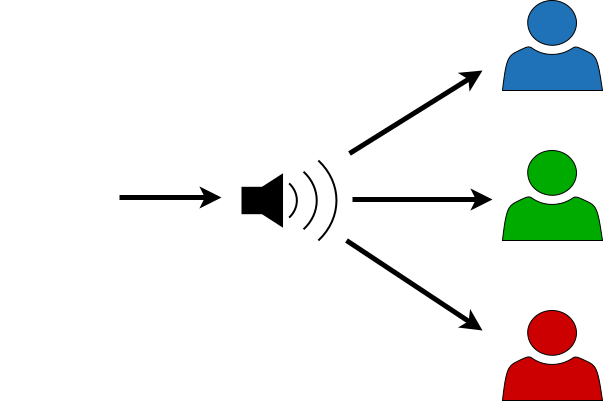
\includegraphics[width=0.45\textwidth]{speech_no_adapt}
		\label{fig:output_not_adapted}} 
	\hfill % no empty line here to avoid staring a new paragraph (figures will be vertically aligned)
	\subfigure
	[An illustration of a device's output, which is \emph{personalized} for each user.
	A different, customized spoken output (in blue, green, and red) is played to each user.]
	{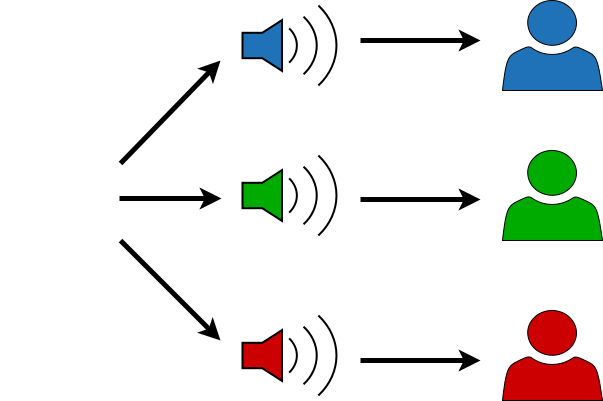
\includegraphics[width=0.45\textwidth]{speech_adapt}
		\label{fig:output_adapted}}
	\caption
	[Static vs.\ adaptive spoken output]
	{Schematic comparison between an interaction with static spoken outputs (on the left) and an interaction with adaptive (i.e., personalized) spoken outputs (on the right).
		The system that adapts to the user makes the interaction tailored to the user's behavior.}
	\label{fig:output_comparison}
\end{figure}

\todo[inline]{taken as-is from SIGdial 2018 subbmitted version. not everyhing belongs here (maybe subsection above?), and the relevant parts should be expanded}

According to \citet{Pardo2006phonetic}, phonetic convergence is defined as an \emph{increase in segmental} \citep[e.g.,][]{Pardo2010conversational, Smith2007prosodic} \emph{and suprasegmental} \citep[e.g.,][]{Walker2015repeat, Shockley2004imitation} \emph{similarity between two interlocutors}.
In contrast to \emph{entrainment}, we use the term \emph{convergence} to describe dynamic, mutual, and non-imposing changes, with potentially non-polarized realizations.
Phonetic convergence has been found in both conversational \citep{Pardo2006phonetic, Lewandowski2012talent} and non-conversational \citep{Babel2014novelty, Shockley2004imitation} scenarios.
There is evidence for phonetic convergence being both an internal mechanism \citep{Pickering2004behavioral} and socially motivated \citep{Kim2011phonetic, Giles1991CAT}.
For instance, convergence \citep{Giles1973mobility} or divergence \citep{Bourhis1977distinctiveness} is triggered with decreasing or increasing social distance between interlocutors, respectively.
Experimental studies on several aspects of phonetic convergence, using a range of methods, have been carried out, e.g., by \citet{Pardo2013measuring, Nielsen2011specificity, Shockley2004imitation}.

Previous studies of phonetic convergence in spontaneous dyadic conversations have focused on speech rate \citep{Schweitzer2016exemplar} and timing-related phenomena \citep{Putman1984conception}, pitch \citep{Gessinger2018pitch, Schweitzer2017visibility}, intensity \citep{Levitan2011measuring, Natale1975convergence}, and perceived attractiveness \citep{Michalsky2017pitch}.
Phonetic convergence is often examined in the scope of shadowing experiments, in which the participants are asked to repeat utterances spoken by an interlocutor \citep{Pardo2017phonetic, Dias2016visibilivty, Walker2015repeat}.
This is typically done with single words as targets.
The experiment showcasing our system in \cref{sec:showcase} uses whole sentences as stimuli, in which the target features are embedded, making it a semi-conversational \ac{hci} setting.

% \input{chapters/introduction/spokendialoguesystems}
\chapter{Spoken Dialogue Systems}
\label{chap:spoken_dialogue_systems}

\lettrine{T}{his} chapter gives an overview of the \aclp{sds} paradigm, including common architectures, different system types, and evaluation methods.
The concept of adaptive \aclp{sds}, which is a core idea in this work, is introduced as well, along with examples of adaptation on different levels.

\pagebreak

%\section{What is a spoken dialogue system?}
%\label{sec:what_is_a_sds}

\todo[inline]{here talk about what is a dialogue, a spoken dialogue, turn, when an interaction becomes a dialogue (is every interaction with a machine is a dialogue system?), etc. can really use the introductions given by Olga in the SDS seminar}

Nowadays, \acfp{sds} are used in various forms in our everyday life.
Giving users all the features of a responsive (sometimes personalized, see \cref{subsec:personal_assistants}) dialogue system with the advantage of using voice to communicate, leaving the hands free to perform any other action, such as driving.\\

In recent years, the market for commercial \acp{va} has rapidly grown.
For example, Microsoft Cortana had 133 million active users in 2016 \citep{Osborne2016why} and Echo Dot was Amazon's best-selling product between 2016 and 2018 \citep{Dickey2017echo}.
Furthermore, \SI{72}{\percent} of people who own a smart speaker say they often use their devices as part of their daily routine \citep{Kleinberg2018ways}.

\todo[inline]{give examples of commercial systems and places where SDSs are used}

\section{Types of spoken dialogue systems}
\label{sec:types_of_sdss}

\todo[inline]{short general introduction explaining the term ``computer-based'' agent as a overarching term for all of the other listed below.}

\begin{table}[tb]
	\centering
	\caption[Types of \aclp{sds}: Task-oriented vs.\ Chit-chats]{A comparison between task-oriented \acp{sds} and chatbots.}
	\label{tab:sds_types}
	\begin{tabulary}{\linewidth}{>{\bfseries}lCC}
		\toprule
							&   {\large \textbf{Task-oriented}}																	& {\large \textbf{Chit-chats}}													\\
		Goal				&	Helps the user achieve a specific, defined goal													& No specific goal, aims to converse as naturally and continuously as possible	\\
		Applications		&	\Aclp{pa}, \acl{cnc} systems, integrated voice-activated systems for cars, reservations, etc.	& Chatbos, social robots, conversational AI										\\
		Domain				&	Domain-specific, possibly multi-domain															& Aims to be domain-free (a.k.a.\ open domain)									\\
		Modeling			&	Statistical models and/or handcrafted rules 													& Typically sequence-to-sequence models with no-go filters						\\
		Evaluation			&	Task completion rate and completion time, number of turns (+ subjective criteria) 				& Chat length, relevant replies ratio, general user satisfaction				\\
	
		\bottomrule
	\end{tabulary}
\end{table}

\subsection{Personal assistants}
\label{subsec:personal_assistants}

\Acp{pa}\ldots

A big advantage of \acp{va} is their simple operation.
Using nothing but speech commands, users can perform tasks like playing music, searching the web, shopping online, etc.
In the future, we are likely to witness an ever-growing presence of devices with spoken interaction capabilities, like speech-activated cars, hands-free medical assistants, and intelligent tutoring systems.
This will increase the demands on voice-activated devices even more, as they will need to support more functionalities in a way that is comfortable and intuitive for the users.
Additionally, it can be expected that such devices will be used not only by individuals, but also in more social contexts, i.e., where multiple humans are involved.


Besides making the operation of such voice-activated systems simple and user-friendly, \acp{pa} also aim to let users interact with them in a familiar, natural manner.
One property of natural interactions is the tendency to accommodate to the specific situation and interlocutors to make the interactions more fluent and efficient \citep{Giles1991CAT,Gallois2015CAT}.
Linguistic accommodation is one aspect of this phenomenon, and it is found in various \ac{hhi} experiments \citep[e.g.,][]{Pardo2017phonetic,Schweitzer2017social}.

\subsection{Intelligent speakers}
\label{subsec:intelligent_speakers}

\Acp{pa} are sometimes integrated into a loudspeaker that can be placed in a central spot at home or in an office\ldots

\subsection{Chatbots and social robots}
\label{subsec:chatbots}

Chatbots (sometimes also called \emph{chatterbots} or \emph{chitchat bots}) are a\ldots

\todo{write a bit about history of chatbots (start with ALICE)}

Chatbots have been used in various domains such as education \citep{Benotti2014engaging, Kerly2007bringing}, culture heritage \citep{Pilato2005expert}, healthcare \citep{Kowatsch2017text}, software development \citep{Lebeuf2017software}, and others \citep{Shawar2007chatbots}.

\subsection{Embodied agents}
\label{subsec:embodied_agents}

\subsection{Virtual agents and virtual humans}
\label{subsec:virtual_agents}

Also known as \textit{avatars}, these...

\section{Architecture of spoken dialogue systems}
\label{sec:architecture_sds}

\todo[inline]{explain that this is a generic, symmetric architecture. there are sometimes some extensions or sub-components to some of the modules}
\todo[inline]{explain that each of the components is a research area by its own}

\begin{figure}[t]
	\centering
	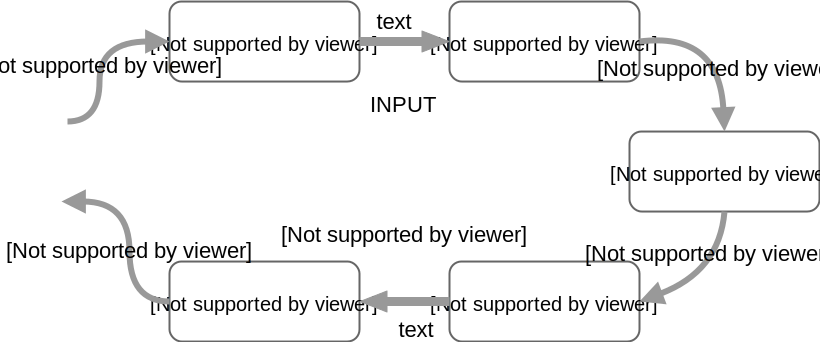
\includegraphics[width=\linewidth]{sds_architecture}
	\caption[Architecture of a spoken dialogue system] {
		A typical architecture of a spoken dialogue system.
		The interaction lifecycle is symmetric, and for each analysis input step there is a corresponding generation output step.
		The exchange usually starts with a user spoken utterance and ends with the system's spoken response.
	}
	\label{fig:sds_architecture}
\end{figure}

Each of a the components shown in \cref{fig:sds_architecture} is a whole research area by itself.
Brief overviews is given here, along with some systems and implementation that can be used for each of these \ac{nlp} task:

\subsection{Automatic speech recognition}
\label{subsec:automatic_speech_recognition}

\subsubsection{Tools}
\label{subsubsec:tools_asr}

\subsection{Natural language understanding}
\label{subsec:natural_language_understanding}

\todo[inline]{be sure to mention the term \enquote{intention}}

\subsubsection{Tools}
\label{subsubsec:tools_nlu}

\subsection{\Acl{dm}}
\label{subsec:dialogue_management}

\todo[inline]{short-mid-length intro to this. about purpose, importance, "core of the SDS", etc.}
\ldots is typically divided into \emph{Belief Tracker} and \emph{Policy}.
\todo[inline]{Now explain about each of them. former is about past turns and anticipating the user's intent, latter is about future responses and what response best matches the user's needs/expectations. mention the use of Reinforcemnet Learning, since it is used when feedback from user is used to improve a system. there are probably papers where this is used.}
\todo[inline]{also explain that this is the part that is connected to external resources, if necessary}

Another component of the \ac{dm} is the \emph{domain}\ldots
Some external knowledge base can be connected as well\ldots
The domain determines what the system can talk about and react to, and to what extent.
\todo[inline]{examples of (simple) domain}
\todo[inline]{combining domains and extending domains, e.g. using crowd sourcing or machine learning}
\todo[inline]{breadth vs.\ depth of domain in SDS (variety vs.\ complexity). replicate the graph Milica showed in her talk (x-axis is breadth and y-axis depth, with some examples along combinations of the axes.)}
\subsubsection{Tools}
\label{subsubsec:tools_dm}

\subsection{Natural language generation}
\label{subsec:natural_language_generation}

\subsubsection{Tools}
\label{subsubsec:tools_nlg}

\subsection{Text-to-speech synthesis}
\label{subsec:text-to-speech_synthesis}

\subsubsection{Tools}
\label{subsubsec:tools_tts}

\section{Adaptive spoken dialogue systems}
\label{sec:adaptive_spoken_dialogue_systems}

\todo[inline]{taken as-is from the submitted version of SIGdial 2018 paper, add more based on existing adapting systems on different levels. need to expand, and add detailed parts about each of the things that can be adapted. get more names of implemented system (maybe even pictures), and mention algorithms etc.}

Various studies have investigated entrainment and priming in \acp{sds}, aiming to better understand \ac{hci} dynamics and improve task-completion performance.
\citet{Lopes2013automated, Lopes2011primes}, for example, focused on dynamic entrainment and adaptation on the lexical level.
Others, like \citet{Nenkova2008high}, concentrated on word frequency.
\citet{Parent2010lexical} examined changes in both lexical choices and word frequency using the \emph{Let's Go} \ac{sds} \citep{Raux2005letsgo}.
While these studies addressed the changes in experimental, scripted scenarios, the theoretical foundations for studying these changes in spontaneous dialogue exist as well \citep{Brennan1996lexical}.
\citet{Gasic2013policy, Levin2000stochastic} provide examples of online adaptation for dialogue policies and strategies.

It is important to note that while all of the studies mentioned above examine various aspects of dialogues, none of those are related to speech -- the primary modality used to interact with \acp{sds}.
Studying convergence in speech in an \ac{hci} context is made possible with more natural synthesis technology, which gives more fine-grained control over parameters of the system's spoken output.
\todo{need references here?}
Many systems that deal with adaptation of speech-related features focus on prosodic characteristics like intonation or speech rate.
\citet{Levitan2014acoustic} sheds light on acoustic-prosodic entrainment in both \ac{hhi} and \ac{hci} via the use of interactive avatars.
\citet{Bell2003prosodic} found that users' speech rate can be manipulated using a simulated \ac{sds}.
Similar results were found when intensity changes in children's interaction with synthesized \ac{tts} output were examined \citep{Coulston2002amplitude}.
A technical overview of the development of adaptive \acp{sds} is given by \citet{Levitan2016implementing}, where speech rate and intensity are manipulated and entrained by the system.

All of the above provide solid ground for further investigation of phonetic convergence in \ac{hci} using \acp{sds}.

\section{Evaluating spoken dialogue systems}
\label{sec:evaluation_of_sdss}

\ldots Therefore, evaluation of \acp{sds} depends on the purpose of the systems, which can be divided into two types, namely \textit{\aclp{tds}} and \textit{\aclp{ngs}}.

\subsection{Task-driven Systems}
\label{subsec:task-driven_systems}
[doesn't really evaluate the \ac{sds}, but it's ability to predict what task should be performed]
[typically part of a bigger system (which has a set of tasks it can perform (e.g. personal assistant))]

\subsection{Non-goal Systems}
\label{subsec:non-goal_systems}

A \acf{ngs} is a \ac{sds} that does not necessarily aim to complete a specific task (unlike \acp{tds}).
Its purpose is, then, more general and there might not even be a defined purpose for it.
Chatbots (see \cref{subsec:chatbots}) are a good a example for a \ac{sds} that typically isn't used for accomplishing a practical task like getting information or operating a device.
Instead, they are used as a long-term social companion (be it at home or as part of a mobile device) and even merely for entertainment. \todo{references for both examples}
Since such systems don't help achieving a defined goal, it is not possible to evaluate their performance based on how well (or whether at all) this goal task was carried out.
There is a need therefore for another, more long-term and interaction-oriented method rather than a task-oriented method.
On the one hand, from the \ac{hci} point of view, the advantage of such methods is that they evaluate the dialogue capabilities of the system and not merely it's ability to map speech patterns or keywords to a set pre-defined actions.
On the other hand, however, the problem in such methods is that it is much harder to define metrics when the goal of the interaction is not completely defined.
There are two approaches to solve this issue:
The first is defining the 


\part{Experiments}
\label{part:experiments}

\chapter{Vocal Accommodation in Real-World Sales Calls}
\label{chap:conv_analysis}

\lettrine{V}{ocal} accommodation occurs in spontaneous \acl{hhi}.
Its effects are investigated in this chapter using a collection of authentic sales calls.
As speaking is an essential part of sales representatives' everyday work, controlling their it is key for their deals' success.
In addition to the extent of the effects, it is also examined which speaker initiated them.

\pagebreak

\acresetall

\section{Harnessing speech alignment for conversation intelligence}
\label{sec:conversation_intelligence}

Sales leaders have always been impelled to be able to reason why some of their representatives (henceforth \emph{reps} or \emph{\acp{ae}}) consistently attain and even exceed their goals while others do not \citep{Kovac2017its}.
Yet, sales executives rely on data that is inherently flawed, as it is based on reports from sources like \ac{crm} systems.
Such systems only contain \enquote{dry} details about deals' stage, along with high-level numeric data and some, typically subjective, estimations regarding their potential in the following stages.
That leaves the executives in the dark regarding the happenings at the front lines and the small-scale, day-to-day conducts and modi operandi, which are critical for the \acp{ae}' success.
As a result, the reasons for losing or winning a deal often remain a riddle, making sales seem like art based on anecdotes rather than a scientifically explainable practice \citep{Yohn2016best, Martin2017six}.
In his seminal book, \citet{Gladwell2006tipping} states that \textquote[p.\ 83]{Part of what it means to have a persuasive personality is that you can draw others into your own rhythms and dictate the terms of the interaction}.
Supporting that, \citet{Orlob2018nine} found that star reps\footnote{Sales representative whose performances (and specifically their closed-deals rate) are exceptionally high are often referred to as \emph{star reps}.
The specific criteria typically include a wide range of behavioral and business metrics, but those are defined internally per company and do not have a common absolute definition.} are able to make prospects increase their speaking rate to match theirs, bringing the two sides closer with respect to this speech property.
However, the scientific analysis is far from their everyday work, and such phenomena are passed on as general tips and are not taught or explained in detail to the \acp{ae}.
\Ac{c-iq} systems aim to bridge over this gap and connect the scientific side of sales to the field to help reps to improve their performance using measured, interpretable methods.
Being part of verbal interaction, vocal accommodation is a facet that can shed light on certain processes occurring during a sales call.
Indeed, this phenomenon has been given attention in analyses and evaluations of \acp{ae}.
It was found, for example, that distinguished sales reps let the prospects talk more and keep certain parts of the calls shorter than low-performing reps \citep{Orlob2017winning}.

\Acf{f0} can be interpreted and explained by people with no phonetic training, like \acp{ae}.
Furthermore, speakers can easily control it, making it a tangible tool for the \acp{ae} to exploit in their sales calls.
This, as opposed to more complex acoustic features like \acp{mfcc} or changes in the \ac{ltas} that are often used in phonetic accommodation studies \citep[e.g.,][]{Levitan2011measuring, Borrie2019syncing} and are hard to directly control during a conversation.
For this reason, the analysis presented in this chapter focus on \ac{f0}, although other suprasegmental features showed similar effects.
For this, a large-scale corpus of real-world sales conversations was collected (\cref{sec:dataset_calls}).
Beside the size advantage, the use of such a corpus takes the study of vocal accommodation out from the controlled laboratory environment into the wild for a practical goal.
The conversations in this corpus are therefore highly flexible and generally structure-free, unlike lab experiments like those presented in \cref{chap:shadowing_in_sung_music_and_human_computer_interaction}.
It is also important to note that beside the overall goal of closing a good deal, there are no specific instructions given to the speakers on both sides regarding how to speak or what to say.
By extension, they are also more authentic and spontaneous, since the interlocutors are driven solely by their own behavior and motivation to succeed and are not given an artificial temporary role.
\Ac{crqa} \citep{Zbilut1998detecting}, a bivariate correlation technique, was used for the analysis (\cref{sec:crqa}).
This method finds instances where coordinates of two time series occur close to each other within a certain radius in a phase-space continuum.
Since \ac{crqa} evaluates the degree to which the similarity of two time series changes over time and can also determine the leading relationship between them, it is suitable and informative for analyzing accommodation.
The contributions of this study are therefore both in the methodology for measuring accommodation and its practical application in a real-world scenario.

\subsection{\Acl{c-iq}}
\label{subsec:conversation_intelligence}

The way people communicate and behave in inter-person situation influences the manner in which conversations unfold.
These influences can be analyzed and interpreted to uncover conversation-level trends, which may differ from the linear turn-by-turn changes.
\Acf{c-iq} is a relatively newly coined term and a field of research that flourished due to advancements in neuroscience, communication science, and \acl{ml}.
It complements other types of human intelligence, like \emph{emotional intelligence} \citep[c.f.\ \emph{Theory of Multiple Intelligences}][]{Gardner1983frames, Davis2011theory}, as the ensemble of conversational aspects in human communication \emph{beyond the surface words and shared information}.
\citet{Glaser2016conversational} explains and demonstrates how \ac{c-iq} can be learned and improved, with emphasis on the ability to gain trust and maintain more successful communication.
Although \ac{c-iq} comprises many further aspects that are beyond the scope of this work, the overarching idea that improving communication quality is a skill that can be learned is highly relevant for vocal accommodation but has not been explored in previous work.

Narrowing down this broad idea, \citet{SilberVarod2018human} discusses how conversations can be \emph{managed}.
This includes both the structure and evolution of a conversation over time and the dynamics between the interlocutors' based on their roles in it.
Noticeably, it is concluded that some speech-related phenomena in conversations tend to be more complex and unpredictable than they seem in their surface form.
One of those phenomena is phonetic entrainment, which was found in long-term influences of the speakers on each other.
Such works dealing with managing spoken interactions become even more relevant with the growing interest in intelligent conversational systems for personal usage \citep{Mehr2017artificial}.
Recently, the importance of \ac{c-iq} has pervaded the enterprise sector and created new businesses.
Two main motivations were the utilization of computer-based customer services \citep{Gnewuch2017towards} and the use of conversation intelligence services for inside sales calls to train \acp{ae} and improve their performance \citep{Orlob2017winning, Orlob2017separates}.

\subsection{Inside sales}
\label{subsec:inside_sales}

In recent years, many companies have adopted the concept of \emph{inside sales}, where \ac{b2b} sales are done using web-based conferencing solutions, as opposed to face-to-face meetings with the clients.
Recent technological advancements allow automatic recording and transcription of those inside sales calls and aggregation of large-scale datasets.
These datasets include the audio of the calls and sometimes annotations such as the speaker turns and performance rating of the \ac{ae}.
These conversations have a typical process:
First, a \ac{sdr} reaches out to a potential client (the \emph{prospect}) who has expressed interest in the company's product, which initiates a \emph{lead}.
Subsequently, the \ac{sdr} shares basic details about the product and how it can help the prospect.
Finally, if the \ac{sdr} has managed to elicit initial interest, the lead turns into an \emph{opportunity}, and a demo call with a sales representative is scheduled.
Such demo calls are often done using a web conferencing tool, such as Zoom\footnote{\url{https://zoom.us}} or GoToMeeting\footnote{\url{https://www.gotomeeting.com}}, which allows both sides to share their webcams and screens.
A collection of such initial opportunity calls is analyzed in here (\cref{sec:dataset_calls}).
It is known in the \ac{b2b} industry that since these calls are the first personal contact, the behavior and verbal skills of the \ac{ae} have a large weight in the success of the call.

\subsection{Influence of speaker roles}
\label{subsec:speaker_roles_and_influences}

Although accommodation is not a traditional measure in \ac{c-iq}, there have been attempts to use it as an additional factor for evaluating conversations.
\citet{Glaser2016conversational} emphasizes the importance of the turn-level alignment between speakers in a business call.
Lack of alignment may result in a skeptic and even resisting behavior that might lower the success chances of the call \citep[see also Table 2 in][]{Glaser2014conversational}.
At the very least, this demonstrates effect of interlocutors being attentive not only to the content of the conversation, but also to the way it is delivered.
In \ac{b2b} calls, this is especially relevant for the \acp{ae}.
\citet{SilberVarod2018human} shows how convergence effects indicate power relations facets of \ac{c-iq} analyses.
Specifically, speaker \enquote{dominancy} is often hard to spot on the surface, but becomes more prominent when examining the vocal relations between the speakers.
Furthermore, \citet{Abrego2011effects} discuss how the judgment of a speaker's role in a conversation influences the phonetic productions and vice versa.
Analyses like these improve the understanding of vocal behaviors in \ac{hhi}.
The idea of speakers' behavior being modified due to their role in the conversation and their perception of the other interlocutor is a key concept for the presented study.

\section{Dataset and feature extraction}
\label{sec:dataset_calls}

A collection of real-world calls with similar characteristics to those described in \cref{subsec:inside_sales} was used in the study presented here.
These calls were all made by trained sales representatives and were aimed at high-stakes deals\footnote{In this case, around US\$\num100,000 each, as opposed to occasional mass calls to random people for selling small products where the deals are very small in comparison.
The reps know that their performances are evaluated, pushing them to do their best in every single call.}.
To make the collection more homogeneous, calls of a single sales company were selected.
Another constraint was that the collection comprised only calls from a very early stage of the sales opportunity (see \cref{subsec:inside_sales}) that is also the first encounter between the participating \ac{ae} and the prospect.
Therefore, the observed behavior patterns in these conversation are not influenced by the previous verbal interactions between the two speakers.
the structure of these calls typically includes an overview of the prospect's business, followed by a deeper explanation of the sold product by the salesperson, and typically further negotiations.
It is important to note that although professional \acp{ae} prepare for these calls as part of the daily work, they are still spontaneous and are in no way scripted.
The calls in this collection were conducted using the Zoom video conferencing platform and were recorded automatically -- without any intervention from either side -- by an external conversation intelligence service.
% Gong.io's system, which provides conversation intelligence services to said company.
The calls were transcribed and diarized using the internal \ac{asr} system of the service.
Participants were notified of the recording, in compliance with all relevant laws and rights.

In total, 708 calls were analyzed, spanning more than \SI{442}{hours} (mean 37.5 $\pm$15 minutes).
Furthermore, only calls longer than 15 minutes were selected, as shorter calls are often unsuccessful connection attempts or brief updates that are not representative of the desired conversation structure and dynamics.
A single \ac{ae} and a single prospect participated in each call.
Call recording started immediately following the first greet from the prospect's side, and stopped when the \ac{ae} terminated it.
This eliminates segments during which one party is waiting for the other to join, and keeps only segments where both parties are present.
%The 26 \acp{ae} (12 female) in these calls formed 87 unique interlocutor pairs with different prospects.
Each prospect only ever spoke with one of the 26 \acp{ae} (12 female).
Both interlocutors in all the conversation were native speakers of American English and worked in an English-speaking company.
For the purpose of this study, a call was defined as successful if a follow-up call under a more advanced stage was initiated or when an advancement in the opportunity was marked within one month.
These criteria follow common conventions of measuring success of \ac{b2b} calls\footnote{The benchmarks for successful deals are much more elaborate in practice and usually consider an entire selling process that comprises a series of calls.
However, many of those criteria are not relevant or cannot be enforced in the scope of this study.}.
This resulted in 51 calls (\SI{7.2}{\percent}) being defined as successful, which is within the industry-standard ratio for such early-stage calls.
%Failed calls lasted 37~$\pm$15 minutes on average and successful calls 42~$\pm$16.5 minutes.
%A two-sample Wilcoxon test \citep{Wilcoxon1945individual} between failed and successful call durations yielded a p-value of 0.04 with a confidence level of \SI{95}{\percent}, confirming their differentiable distributions.
%It goes without saying that the labels of both criteria are noisy, as sales opportunities might be lost due to various other factors.
%To minimize such cases, calls done by personnel that are not sales people in the customer companies were filtered out.
%Following that, we hypothesized that successful sales calls would show more distinct speech patterns and vocal accommodation behaviors than unsuccessful calls.

To increase temporal resolution, the audio signals were split into two-second slices (cf.\ \cref{sec:analysis_hhci}).
This increases the number of datapoints the \ac{crqa} considers.
Splitting the turns also creates equal, consecutive, and more comparable time units in the conversations without introducing artificial boundaries by dividing it into a pre-defined number of parts based on some arbitrary criterion.
The slicing was done per turn, so that a slice contains only the speech of a single speaker.
Any remainder of a turn got a slice of its own.
When a speaker was not speaking (e.g., during the turn of the other interlocutor), it was assumed that the last produced value was maintained until the speech is renewed and a new value can be measured.
This way, no discontinuities are created and the same number of datapoints can be extracted for both speakers to create a better temporal representation of the conversation.
Feature extraction was done using the system described in \cref{chap:web-based_responsive_spoken_dialogue_system} \citep[and see][]{Raveh2018Specom}.
The values were measured using Praat \citep{Boersma2018praat} scripts that extracted the \ac{f0} value from the middle of each slice.
Afterward, the list of measures was turned into two equally long time series:
First, the values for each speaker were separated into two lists.
Subsequently, missing values, e.g., due to non-speech slice, were replaced by the most recent valid value of their respective speaker, as motivated above.
Finally, if there were missing values at the beginning of a list, the first valid value of that list was used, under the assumption that the first utterance represents the immediate time prior to it.
The resulting two lists had the same number of values representing the same timestamps along a single conversation, and were used as the input time series for the \ac{crqa}, which can be assumed to be non-seasonal and non-stationary.
This process was performed independently for each conversation.

\section[\Acl{crqa}]{\Acl{crqa} for measuring vocal accommodation in conversations}
\label{sec:crqa}

\subsection{Capturing accommodation with \acs{crqa}}
\label{subsec:capturing_behaviors}

Depending on the circumstances, \ac{hhi} may involve different communication channels, such as facial expression, hand gestures, and eye gaze.
The analyses here concentrate on the phonetic level, as it is the primary modality used for conveying information in sales calls, even when video or screen sharing functionalities are available as well.
It has been shown in studies based on \ac{cat} (\cref{sec:communication_accommodation_theory}) that
mutual vocal adjustments in \ac{hhi} increase the success rates of conversations \citep{Pickering2004behavioral} and affects the social distance between speakers \citep{Schweitzer2017social}.
Accordingly, effects of the same nature have been found in \ac{b2b} sales calls as well \citep{Orlob2018roi}.

Linear methods for measuring accommodation rely on the chronological, turn-by-turn order of the interaction.
As discussed in \Cref{subsec:limitations_of_did,fig:accommodation_types}, these methods are limited to the detection of local effects that evolve gradually across adjacent turns.
Non-linear methods, on the other hand, do not rely on turn adjacency and can find long-term relations between the speakers' speech productions on the conversation level.
For instance, accommodation may occurred at some point in the beginning and be continued at a later time.
This is especially useful for long interaction, like the sales calls in the corpus used here, where the insights from more general view are useful for improving performance.
This encourages treating the interactions as continuous event rather discrete parts, and opens a variety of time series analysis methods.
\Ac{crqa} is one such method, which offers more than the direct comparison of large pre-defined chunks of neighboring turns, as is typically done in accommodation studies in spontaneous conversations \citep[e.g.,][]{Levitan2013entrainment, Rahimi2018weighting}.
It utilizes phase-space embedding, which describes the temporal evolution of trajectories of a dynamic system by projecting their embedding onto some common space.

An overview of \ac{crqa}is given by \citet{Wallot2018analyzing}.
At its core, this method compares delayed instances of the phase-space trajectories of two time series.
This allows for finding more general patterns in the time series characteristics and how they interact.
It is especially suitable for studying accommodation and related phenomena, as it detects times in which the time series (here, the speakers' productions) are similar.
Moreover, it can mathematically show which of the time series lead the alignments or whether the changes were done in synchrony.
This is useful for describing different the types of accommodation described in \cref{subsec:variation_types}, like synchrony and alignment.
\Ac{crqa} has already been used in \ac{hhi} research.
For instance, \citet{Duran2017conversing} used it for analyzing and predicting speech differences in scenarios with disagreement and deception tasks.
A similar method was used by \citep{Borrie2019syncing} to measure conversational entrainment for assessing speech pathology.
It was found that sessions with longer periods of synchronization were rated as more successful by therapists.
This is a good example of a cooperative interaction with a common goal that accommodation contributes to its success.
In sum, \ac{crqa} can be used to objectively quantify and describe accommodation between speakers dynamically across entire conversations.
\Cref{subsec:recurrence_detection,subsec:parameters_crqa} explain the technicalities of \ac{crqa}, how its output can be interpreted, and how it is used in the study presented in this chapter.
%
\begin{figure}
	\centering
	\includegraphics[width=\linewidth]{crqa_plot_115993376241473405}
	\caption[\acs{crqa} analysis of pitch in a sales call]
		{A recurrence plot generated for one of the analyzed conversations.
		The y-axis marks the conversation timeline, in slices, of the \ac{ae}, and the x-axis of the prospect.
		Each blue dot represents a co-visitation of a similar state.
		Blue dots forming a diagonal line indicate sustained recurrence between the two speakers (see description of NRLINE in \cref{subsec:output_values} for details).
		Note that the timestamps on the axes are not the slices, but the embedded call time.
		For example, the diagonal structures between timestamps 100 and 200 of the x-axis show such lasting recurrence.
		Diagonal lines above the \acl{los} (\acs{los}; the central diagonal line) indicate that the speaker on the y-axis leads the x-axis, and vice versa for lines below the \ac{los}.
		The blank area between timestamps 220 and 330 of the x-axis point to a portion of the call where the speakers were more distant from each other.}
	\label{fig:crqa_plot}
\end{figure}

\subsection{Recurrence detection}
\label{subsec:recurrence_detection}

\Ac{rqa} is a method for non-linear data analysis that quantifies the number and duration of recurrences within a dynamical system presented by its state-space trajectory, which is typically the realization of a sampled time series.
It was introduced by \citet{Zbilut1992embeddings} and later extended by \citet{Webber2005recurrence, Marwan2002cross}.
A \emph{recurrence} (also, \emph{re-visitation}) is a time in which the trajectory returns to a state it has visited before.
Recurrence can, therefore, be defined as the binary function
%
\begin{equation}
	\label{eq:recurrence}
	R_{i,j} =
	\begin{cases}
		1,	&	\text{if} \quad \lVert \vec{x}(i)-\vec{x}(j) \rVert_d \leq \varepsilon \\
		0,	&	\text{otherwise} \\
	\end{cases},
\end{equation}
%
where $i$ and $j$ are samples of the time series, $d$ is the number of embedding dimensions, and $\varepsilon$ is the threshold radius distance below which two cross-trajectory points are considered similar, as explained in \cref{subsec:parameters_crqa}.
\Ac{crqa} is an extension of \ac{rqa} for analyzing recurrence quantification between \emph{two different} time series rather than a single one.
As such, \ac{crqa} is a quantification technique for non-linear data analysis that describes when and to what extent concurrences (or \emph{co-visitations}) occur in the two time series.
These quantification techniques are based on \emph{recurrence plots} that for each pair of samples $i$ and $j$ from the two time series show the times at which a phase space trajectory is similar, i.e., when $TS_i \approx TS_j$ (and see \cref{fig:crqa_plot}).
The recurrent points $R_{i,j}$ are colored if their value is 1 or remain unmarked otherwise.
The main diagonal of the plot is called the \acf{los}.
A high number of recurrences along this line indicates synchrony between the time series.
However, diagonal recurrence lines can be formed above and below the \ac{los}.
Such diagonals, especially longer ones, represent delayed (lagged) synchrony between the time series and can be used as an assessment of similarity between the processes.
In the context of accommodation, these diagonals imply accommodative processes led by one of the interlocutors.
If the diagonal stretches above the \ac{los}, the speaker plotted on the x-axis leads the accommodation and vice versa.
The closer the diagonal is from the \ac{los}, the faster the process occurred, i.e., the led speaker aligned his behavior to the leading speaker after a shorter time.
This ability to not only detect latent accommodation but also determine its initiator on a fine-grained time scale enables the description and detection of more complex accommodation behavior, such as delayed synchrony (\cref{fig:accommodation_types}).

\subsection{Parameter tuning}
\label{subsec:parameters_crqa}

\Ac{crqa} has three parameters:

\begin{enumerate}
	\item \textbf{Delay} -- estimates the temporal shift required to make the two time series maximally correlated.
	It is measured by the same time unit as the time series (here, two-second slices; see \cref{sec:dataset_calls}).
	
	\item \textbf{Embedding dimensions} -- are the number of dimensions into which the datapoints are embedded.
	These dimensions are delayed copies of the original time series $TS_t$ created by adding a lag $k$ to them.
	Typically, multiple $n$ lags are considered, which create the dimensions of embedding $TS_{t + nk}$.
	
	\item \textbf{Radius} -- determines the margin within which two datapoints constitute a recurrent instance.
	Distances between the datapoints are measured in the embedded space defined by embedding dimensions, using the same unit used for measuring the values of the time series.
\end{enumerate}
%
\begin{figure}
	\centering
	\begin{minipage}{.45\linewidth}
		\centering
		\includegraphics[width=\linewidth]{ami}
		\caption[Average mutual information of time series as function of lag]
			{The average mutual information of the time series values as a function of the lags considered.
			The x-axis shows the considered lags and the y-axis the mutual information index (AMI) in bits.}
		\label{fig:ami}
	\end{minipage}%
	\hfill
	\begin{minipage}{.45\linewidth}
		\centering
		\includegraphics[width=\linewidth]{false_NN}
		\caption[Embedded dimensions optimization]
			{False nearest neighbors percentage as a function of the number of embedded dimensions.
			The x-axis show the considered numbers of embedded dimensions and the y-axis the percentage of false nearest neighbors.}
		\label{fig:false_nn}
	\end{minipage}	
\end{figure}
%
These parameters are a key aspect in \ac{crqa}, and how they are set is decisive for its outcome.
However, although some best-practice guidelines exist, like those suggested by \citet{Coco2014crqa-r}, there is nevertheless no standard way for optimizing these parameters and their determination depend on the nature and characteristics of the data.
An optimization method similar to the one presented by \citet{Marwan2007recurrence} was utilized here.
The average mutual information (AMI) of the time series' shifted instances is defined as 
% from https://www.frontiersin.org/articles/10.3389/fpsyg.2018.01679/full
\begin{equation}
	\label{eq:average_mutual_information}
	AMI\left( TS_{i(t)}, TS_{j(t + \tau)} \right) = \sum_{i,j} p_{ij} (\tau) \log \left( \frac{p_{ij} \left( \tau \right)}{p_i p_j} \right),
\end{equation}
\eqname{Average mutual information (AMI)}\noindent
%
where $i$ and $j$ are values from the two time series, $t$ is the original starting time of the time series, $\tau$ is the amount of shift between the time series, and $p_{ij}$ is the probability that $R_{i, j} = 1$.
Note that only the shift $\tau$ influences this value and not the absolute initial time $t$.
The delay parameter was subsequently determined by finding the lag value $\tau$ that minimizes the average mutual information between the two time series, as follows:
%
\begin{equation}
	\label{eq:delay_opt}
	\hat{\tau} = \argmin_{\tau} \left( AMI\left( t, \tau \right) \right).
\end{equation}
\eqname{Optimization of delay parameter}\noindent
%
%
\addtocounter{equation}{1}
\begin{algorithm}[t]
	\caption{\acs{crqa} radius optimization}
	\label{alg:radius_opt}
	\algorithmcaption
		{\emph{The higher $n$ is (\cref{line:num_cand}), the higher the chance of a \ac{rr} close to the defined \emph{desired RR}.Also note that since \ac{rr} represents percentage of values in the recurrence plot, 100 is its highest possible value.
		Therefore, and since the radii in $R$ are traversed in increasing order, the search stops if this value is achieved (\cref{line:break_at_rr_100}).
		As explained in the text, in the presented studies $n = 20$ and $desiredRR = 10$ \citep[see][]{Coco2014crqa-r}.}}
	\DontPrintSemicolon
	\SetKwInOut{Input}{Inputs}
	\SetKwInOut{Output}{Output}
	
	\Input{\underline{$desiredRR$} -- the desired approximated \ac{rr} value\newline
		\underline{$optDelay$} -- the optimized delay\newline
		\underline{$optEmbedim$} -- the optimized embedded dimensions\newline
		\underline{$TS$} -- all values from both time series}
	\Output{radius producing \ac{rr} value closest to the defined desired \ac{rr}\newline}
	
	$n \gets$ number of radius candidates \label{line:num_cand}\;
	$R \gets \{r_i, \ldots, r_n\} : r_1 = 0, r_n = \max(TS)$\;
	$\forall r \in R : \lvert r_i - r_{i-1} \rvert = \lvert r_{i+1} - r_i \rvert$ \tcp*{evenly spread candidates}
	
	$candR \gets \varnothing$\;
	\ForEach{$r \in R$}{
		$currRR = crqa(ts_1, ts_2, optDelay, optEmbedim, \ldots\footnotemark).RR$ \tcp*{RR with candidate}
		$candR = candR \cup currRR$\;
		\uIf{$currRR = 100$}
		{\emph{break} \label{line:break_at_rr_100} \tcp*{\ac{rr} cannot be higher than 100}
		}
	}
	$optRadius = \displaystyle\argmin_{r \in R}(\lvert candR_r - desiredRR \rvert)$\;
\end{algorithm}
\eqname{Radius optimization algorithm for \acs{crqa}}
\footnotetext{As calculated by the \ac{crqa} package for R \citep{Coco2014crqa-r} with the additional arguments (unlisted in the algorithm itself) \emph{rescale=0, normalize=0, minvertline=length(ts1) / 100, mindiagline=length(ts1) / 100,} and \emph{tw=0}.}
%
The lag with the \emph{lowest} average mutual information was selected, regardless of whether and when the values started to level off.
This provides a delay that is not too short to miss the mutual differences, but also not too long to lose the dependency between the time series.
The number of embedding dimensions was obtained using false nearest neighbors \citep{Kennel1992determining}.
This algorithm determines the minimum embedding dimension necessary to reconstruct the state space of a dynamical system with time delay embedding, as explained by \citet{Abarbanel1993local}.
A neighborhood diameter equal to the standard deviation of the time series was used, and a limit of 20 embedding dimensions (which was never reached) was set.
\Cref{fig:ami,fig:false_nn} show examples of mutual information and false nearest neighbors optimizations using the data used for the study presented here.
Following that, the radius was calculated in two steps (\cref{alg:radius_opt}).
First, the goal \ac{rr} and a list of potential radii were initialized.
Here, the goal \ac{rr} was set to \SI{10}{\percent}, which is considerably higher than in similar studies, e.g., \SIrange{2}{5}{\percent} in \citet{Coco2014crqa-r}.
Setting the goal \ac{rr} to a higher value results in a stricter optimization that includes only (even) closer recurrences.
The potential radii were generated by evenly spreading 20 candidates from 0 to the maximum value in the time series.
Then, each radius, along with the already optimized delay and embedding dimensions, was used to perform a \ac{crqa}.
A stricter policy was introduced in this step as well, as only recurrence lines longer than \SI{1}{\percent} of the longer time series' length were counted, as opposed to the typical setup that considers lines of any length \citep[e.g., as in ][]{Borrie2019syncing}.
With an average length of \SI{37.5}{minutes}, this means that only lines longer than 11 time units (22 second) were considered.
% note: calculated by multiplying 37.5 minutes * 60 to get seconds, then divide by 2 since each time unit (slice) was 2 seconds and again divide by 100 to get one percent of it.
This ensured that only long-term recurrences were taken into account, and shorter, possibly more random effects, were filtered out.
Finally, the candidate radius that resulted in the smallest absolute distance from the goal \ac{rr} was chosen to perform the \ac{crqa}.
This process is summarized in \cref{alg:radius_opt}.
The optimization processes of all three parameters were done separately for each conversation.

\section{Analysis}
\label{sec:analysis_hhi}

Time series-based analysis methods like \ac{crqa} can be used in many ways.
The measures used in this study are explained in \cref{subsec:output_values}, followed by the results they yielded for the sales calls collection in \cref{subsec:results_hhi}.

\subsection{\Acs{crqa} output values}
\label{subsec:output_values}

Various measures can be computed based on a recurrence plot\footnote{See detailed overview in \citet{Marwan2007recurrence} and summary with additional measures and examples in \url{http://www.recurrence-plot.tk/rqa.php}.}.
Some deal with the \ac{los} and other diagonals across the recurrence plot, while others consider vertical and horizontal lines.
Below are the definitions of the measures used in this study.
For simplicity, it is assumed that the time series lengths are equal, so that $N_i=N_j=N$.

\begin{description}
	\item[\Acf{rr}] -- The percentage of recurrent points in the plot, i.e., the percentage of similar values between the two time series out of all the values as calculated using the parameters described in \cref{subsec:parameters_crqa}.
	It is defined as
	%
	\begin{equation}
		\label{eq:rr}
		RR = \frac{1}{N^2} \sum_{i=1}^{N_i} \sum_{j=1}^{N_j} R_{i,j}.
	\end{equation}
	\eqname{-- 4.4.5 \acs{crqa}-based measures: RR, DET, L, maxL, and ENTR}
	%
	This number corresponds to the amount of colored points in the recurrence plot.
	The lengths $N_i$ and $N_j$ of the time series are often -- but not necessarily -- equal
	
	\item[Determinism (DET)] -- The percentage of recurrences forming diagonal lines in the recurrence plot given a minimal length threshold $l_{\min}$.
	It is calculated as
	%
	\begin{equation}
		\label{eq:det}
		DET = \frac{\sum_{l=l_{\min}}^{N} l P(l)}{\sum_{l=1}^N l P(l)},
	\end{equation}
	%
	where $l$ is the length of a line and $P(l)$ is the length histogram of all diagonal lines.
	Note that $l=1$ refers to lines of length 1, i.e., a single recurrence point.	
	Similarly, $l=2$ are lines spanning over two timestamps (shortest lines possible).
	Short lines lengths are very forgiving in the case of accommodation, for they can be formed abundantly and therefore not necessarily indicate a meaningful accommodation process.
	For this reason, $l_{\min}$ was set to $\frac{N}{100}$ in this analysis, as detailed in \cref{subsec:parameters_crqa}.
	
	Another measure, Laminarity (LAM), can be calculated the same way, but for the vertical lines in the plot.
	In that case, a $v_{\min}$ is defined and $P(v)$ provides the histogram of vertical line lengths.
	
	\item[Number of lines (NRLINE)] -- The total number of lines $N_l$ formed in the recurrence plot per the definition of the \emph{DET} measure.
	In the context of accommodation, this is the number of accommodation \enquote{instances} between the two speakers lasting at least $l_{\min}$ time units.
	Also referred to as \emph{sustained recurrence} by \citet{Borrie2019syncing}, this measure not only shows the number of detected accommodation effects, but also how long they last.
	
	\item[Average length (L)] -- the average length of the diagonal lines, i.e., the average total accommodation time between the speakers.
	A higher value indicates longer average individual accommodation timespans in the conversation.
	It is calculated as
	%
	\begin{equation}
		\label{eq:l}
		L = \frac{\sum_{l=l_{\min}}^N l P(l)}{\sum_{l=l_{\min}}^N P(l)}.
	\end{equation}
	%
	The average length of vertical lines, trapping time (TT), is achieved in a similar way when using the same formula for the vertical line length and the histogram of vertical line lengths.
	
	\item[Maximal length (maxL)] -- The longest diagonal line in the plot (excluding the \ac{los} in \ac{rqa}).	
	This is the longest, uninterrupted timespan over which accommodation between the speakers has lasted.
	It is determined by
	%
	\begin{equation}
		\label{eq:maxl}
		L_{max} = \max_{l} (\{l_i; \ i=1, \ldots, N_l\}).
	\end{equation}
	%
	Similarly, the longest vertical line can be determined by traversing the vertical lines.
	
	\item[Entropy (ENTR)] -- The Shannon entropy of the probability distribution of the diagonal line lengths longer than the minimum length $l_{\min}$.
	Describes the variability of the amount of accommodation instances across the conversation.
	Higher value indicates more varied lengths.
	Based on Shannon's entropy formula, this value is defined as
	%
	\begin{equation}
		\label{eq:entr}
		ENTR = -\sum_{l=l_{min}}^{N} p(l) \ln p(l),
	\end{equation}
	%
	where $p(l)$ is the probability of length $l$ from the lengths probability distribution.
	\item[Normalized entropy (rENTR)] -- The entropy value normalized by the number of lines formed in the recurrent plot.
	This measure describes the length variation across multiple conversations and is therefore not too biased by special characteristics some conversations might have.
\end{description}
%

\subsection{Results}
\label{subsec:results_hhi}

Seven out of the output values described in \cref{subsec:output_values} were measured for all 708 conversations and their distributions were checked for statistical significance.
Since multiple variables are compared here, the Bonferroni correction \citep{Bonferroni1936teoria} was applied, so that the overall error rate across all variables is $\alpha = 0.05$.
Therefore, for a single comparison to be significant, its p-value must be lower than 0.007.
The non-parametric two-sample Wilcoxon test \citep{Wilcoxon1945individual} was used to determine the significance levels.
\Cref{tab:crqa_results} summarizes the means and p-values of these distributions for failed and successful calls.
The \ac{rr} mean value is about 10 in both groups, which matches the goal value set for optimization (\cref{subsec:parameters_crqa}).
Significant differences between failed and successful calls were found for the values DET, NRLINE, and rENTR.
The first two, along with their higher means for the failed calls, indicate more synchronous accommodation instances in the failed calls.
The latter is harder to interpret, especially due to the similar means for successful and failed calls.
It seems that the behavior in both cases is equally predictable across calls, but differently.
One possible factor influencing these behaviors is related to the interlocutor leading the accommodation effect, rather than the fact that it occurs at all, as shown below.
The significant difference in the NRLINE measure stands in line with the findings of \citet{Borrie2019syncing}.
The same tests were performed based on the leading speaker in each conversation (bottom part of \cref{tab:crqa_results}), but no significant differences were found for this criterion.

\begin{table}[t]
	\caption[P-values of the comparison between \acs{crqa} measures in sucess and failed calls]
		{P-values of the two-sample Wilcoxon test comparing the \ac{crqa} output values based on call success/fail and leading speaker along with their respective mean values.
		Significant values based on the adjusted p-value threshold are in bold.}
	\label{tab:crqa_results}
	\begin{tabularx}{\linewidth}{X
								 S
								 S[table-comparator=true, table-space-text-pre={$\ll$}]
								 S[table-comparator=true, table-space-text-pre={$\ll$}]
								 S
								 S
								 S
								 S[table-format=1.4]}
		\toprule
						& {\thead{\acs{rr}}}	& {\thead{DET}} 		& {\thead{NRLINE}}		& {\thead{maxL}} 	& {\thead{L}} 	& {\thead{ENTR}} 	& {\thead{rENTR}} 	\\
		\midrule
		p (deal)		& 0.9					& \bfseries $\ll$0.001	& \bfseries $\ll$0.001	& 0.7 				& 0.07			& 0.1				& \bfseries 0.0058 	\\
		mean success	& 10.1					& 2.2					& 84.0					& 31.3 				& 17.8			& 1.4				& 0.8				\\
		mean fail		& 10.0					& 5.9					& 174.0					& 32.9 				& 15.3			& 1.5				& 0.8				\\
		\rule{0pt}{4ex}\\
		p (lead)		& 0.7					& 0.1					& 0.05					& 0.18				& 0.9			& 0.07				& 0.55				\\
		mean \acsp{ae}	& 10.0					& 6.1					& 186.7					& 35.2				& 15.2			& 1.5				& 0.8				\\
		mean prospects	& 10.1					& 5.4					& 154.4					& 31.2				& 15.7			& 1.4				& 0.8				\\
		\bottomrule	
	\end{tabularx}
\end{table}

To shed more light on the leading role, \acl{cc} was used to determine which interlocutor led the change in behavior.
\Acl{cc} finds the degree to which two time series are synchronized with different lag values..
The correlation between the time series was calculated for each lag, and the value that made the series maximally correlated was selected.
A positive value suggests that the first time series needs to be shifted forward to achieve maximal correlation and vice versa.
In the context of accommodation, this \acl{cc} indicates indicates which speaker was leading the change.
The \acl{cc} function was not limited to a specific range of shifts, so that all possible lags were considered.
The lag associated with the maximal correlation was used to determine the leader.
Since the calls in the collections used here are from the same domain, it is also interesting to examine at which point of the conversation the maximal correlation occurs.
\cref{fig:barplot_conv_leaders} shows the time, in percent, in which the maximal correlation occurred for \acp{ae} and prospects in successful and failed calls.
The difference between the lag position distribution of reps and prospects is significant ($p = 0.0065;\ \alpha = 0.05$).
However, no significant different was found between successful and failed calls for the same leading speaker.
It is also evident that when the reps were leading, they consistently did so at an earlier stage of the conversation, all the more so in successful calls, whereas prospects' lead varied much more and generally happens at a much later time.
%
\begin{figure}
	\centering
	\includegraphics[width=\linewidth]{boxplot_ccf}
	\caption[Representatives' and prospects' lead-taking times in successful and failed calls]
		{Comparison between the time of the call in which the maximal \acl{cc} occurs.
		The x-axis groups the calls based on the speaker role, and the fill color further separates between successful and failed calls.
		The y-axis shows the conversation timeline in percent (\SI{50}{\percent} marks the middle of the conversation).
		The horizontal lines in the boxes represent the median
		and he notches stand for the \SI{95}{\percent} confident level.
		% The area inside the boxes include the \acf{iqr} of values, the vertical lines outside the boxes show the value within the third quartile + 1.5$\protect\cdot$\ac{iqr}, and the isolated dots are the outliers.
		The significance level calculated with Wilcoxon test comparing the two groups and their subgroups is given above the boxes.}
	\label{fig:barplot_conv_leaders}
\end{figure}
%
Another known conversational element in sales calls is the floor time each speaker gets.
As a general approach, \acp{ae} aim to let the prospect talk as much as possible.
This is known to give them a better feeling during the call, and also give the reps more information and opportunities to understand what the customer wants to talk about.
Indeed, a recommended practice is to track the \emph{speech balance}, i.e., the ratio between the speaking time of the speakers.
Besides speech balance, the frequency and timing of floor switching also provide some insight on the dynamics of the speakers' vocal behaviors.
While each speaker should get a sufficient amount of time to talk, it is also important to take and give the floor to the other interlocutor when necessary.
Long monologues can make the listener lose concentration or lack of expression, which damages the interaction.
Therefore, the \emph{interactivity} of the speakers is important as well.
While speech balance informs about the overall amount of time each speaker talked, interactivity complements this by informing how often a speaker gave the floor to the conversation partner.
These two speech-related properties fit into the overall notion of vocal behavior.
Speech balance was measured by
%
\begin{equation}
	\label{eq:speech_balance}
	speech\_balance = 
	1 - \left| \frac{\displaystyle \sum_{\forall S \in S_A} dur(S) - 
						\sum_{\forall S \in S_B} dur(S)}
					{\displaystyle \sum_{\forall S \in S_A \cup S_B} dur(S)}
		\right|,
\end{equation}
\eqname{Speech balance in conversation}
\noindent
%
where $S_A$ and $S_B$ are the slices in which speakers $A$ and $B$ speak, respectively, and the function $dur$ returns the duration a slice.
The yielded value between 0 and 1 indicates the percentage of the balance in terms of speech times, with 1 standing for \enquote{perfect balance}, i.e., equal talking times for both speakers.
As mentioned above, the overall speech balance only reveals part of the whole picture.
Another part of it is the interactivity in the conversation, which is here defined as the percentage of slices in which floor change occurred after a sequence of longer than 1 slice was calculated.
Sequences below this threshold were treated as backchanneling, which does not indicate speaker change.
Interactivity and speech balance were measure for a superset of the dataset presented in \cref{sec:dataset_calls}.% which consisted of more than 1000 calls.
\cref{fig:speech-balance_success_violin} shows the speech balance scores of successful and failed calls.
On the one hand, it is clear that the lower the balance the more likely it was that reps had more floor time.
The recommendation to avoid imbalance is reflected by the significant difference between balance distribution in successful and failed calls.
On the other hand, prospects are only likely to talk more when the balance score is high, even more so in successful conversations.
This is accentuated by the highly significant differences in both sub-groups.
No significant influences of interactivity on call outcomes were found, and only a weak correlation between speech balance and interactivity was found ($\rho = 0.2$).
%
\begin{figure}
	\centering
	\includegraphics[width=\linewidth]{speech-balance_success_violin}
	\caption[Distribution of speech balance in successful and failed calls]
		{Comparison of speech balance distribution in successful and failed calls sub-grouped by the speaker who had more floor time in individual calls.
		The width of the shapes represent the probability density.
		The inner boxes show the central quartiles of the data.
		The medians are marked by the thick horizontal lines in the boxes.
		The additional horizontal lines mark the \SI{25}{\percent}, \SI{50}{\percent}, and \SI{75}{\percent} quartiles of the data.
		The asterisks above the shapes denote the significance levels of the comparisons between the main groups (successful vs.\ failed) and the subgroups (* $p < 0.05$, *** $p < 0.001$, **** $p < 0.0001$).}
	\label{fig:speech-balance_success_violin}
\end{figure}

\section{Conclusion}
\label{sec:conclusion_hhi}

The study presented in this chapter investigated accommodation occurrences in real-world sales conversations using \acf{crqa}.
Two main properties were examined, namely call success and role influence.
The results show that successful and failed calls significantly differed in three of the \ac{crqa} output values.
Although based on some \ac{hhi} studies it might be hypothesized that recurrence is more likely to occur in successful calls, the means of two of the three values suggest the opposite.
Yet, this stands in line with other studies from sales research that show more \enquote{desperate} behavior from the rep side when a deal is hard to close.
This includes unconsciously showing assimilation towards the prospect and over-emphasizing details, with the hope that it will convince the prospect to close a deal \citep{Orlob2018roi}.
However, these often achieve the opposite effect and are therefore discouraged in the sales industry.
Another possible explanation is that reps give up the lead when a call is on the verge of failing and instead let the prospects lead to give them a better feeling.
This, too, is a known effect in the sales business.
On the other hand, utilizing \acl{cc} lags proved to be useful for differentiating between the leader in the calls.
When \acfp{ae} lead, they tend to do so at an earlier stage than prospects, especially in successful calls.

All these suggests that \acp{ae} do not necessarily always lead the conversation, but know how and when to exploit this technique, consciously or not, to improve their stance in calls.
It can be concluded that accommodation-related characteristics can be found in spontaneous, goal-oriented conversations and be used as a mean of analyzing their effectiveness.
However, despite anecdotal recommendations and recommended best practices, it cannot be claimed that exploitation of these effects \emph{directly influence} calls' success without further investigating, e.g., long-term performances of highly-rated reps.

%Though beyond the scope of this work, three further investigation directions on this topic are suggested here:
%First, deepening the aspect of the relationship between the \acp{ae} and the prospects by examining the mutual changes not only within single calls, but over the course of an entire deal spanning over several meetings.
%This could shed light on long-term changes and connect changes to the success of the deal.
%Secondly, distinguishing between different \acp{ae} to find behaviors of sub-groups or identifying star reps.
%For example, salespersons with higher ratings might be revealed to better exploit accommodation and trigger different behavior on the prospect side to increase their chance of closing a deal.
%Lastly, different methods could be applied to predict the success of a call.
%Specifically, machine learning methods that are good at capturing serial changes, such as recurrent neural networks, can be used to train such prediction models.
%All these directions can also be combined with more features to uncover more consistent accommodation patterns.

% Conclusion
%We have presented a study that examines phonetic accommodation in real-world sales calls.
%The focus was on mutual proximity of \acl{f0} between salespersons and prospects to find both how close they are to each other in general across the call, and how quickly changes in proximity occur and by whom they are initiated.
%This was done by \acf{crqa} and \aclp{cc}, which together provide various measures regarding recurrence between the speakers and who leads the other in terms of \acl{f0} changes.
%A corpus of 708 calls was used for the analyses, which makes it possible to find more global, consistent effects that are not influenced by the design of a specific experimental setting.
%The results show significant differences in some of the values between successful and failed calls, and significant differences between the leading behavior of salespersons and prospects.
%These findings encourage further investigations, like looking for other predictors of successful calls and examining the influence of additional features and factors on the success of calls.

\chapter{Shadowing in Sung Music and Human-Computer Interaction}
\label{chap:shadowing_in_sung_music_and_human_computer_interaction}

\lettrine{A} series of experiments is described in this chapter.
Some of them were designed to determine human behavior in \acl{hhi} and \ac{hci} as a mean of modeling interactions, and others examined the change in reactions of subjects to different adaptation strategies of implemented system as a subjective evaluation method.

\pagebreak

\section{Shadowing paradigm}
\label{sec:shadowing_paradigm}

In a shadowing task, are participant are instructed to provide vocal productions as a reaction to pre-determined stimuli.
It is often used in empirical experiments \citep[e.g.,][]{Goldinger1998echoes} to examine how certain properties of these stimuli influence -- or do not influence -- participants' productions.
A shadowing task is typically preceded by a baseline phase, where the participants provide the same productions without listening to the stimuli.
The stimuli used in the shadowing phase can be determined based on the baseline production, e.g., for intentionally introducing a contrast between with respect to the participants' productions, as done in \cref{subsubsec:procedure_hci}.
A comparison between the production in these two phases indicates whether and to what extent the stimuli had an effect on the participants' productions.
Sometimes a third, post-shadowing phase is added to examine whether the effect -- or lack thereof -- found in the shadowing phase persist when the external inputs are absent.
\Cref{fig:HCIConvFlow} shows a complete flow of the shadowing paradigm used in an experiment.
It is important to note that the baseline for change is not \SI{50}{\percent} (randomly retaining preferred realization or adopting stimulus' form).
Since people are not likely to spontaneously change their speech, the assumption here is that the probability of change represents the influence of the stimulus on the speaker.
More generally, the degree of accommodation can be seen as a speaker's tendency to converge to an interlocutor (cf.\ \emph{sensitivity} property in \cref{sec:parameters}).
\todo{need to say that though it might occur, 100\% convergence cannot be realistically expected}

Vocal accommodation is often studied using shadowing tasks, in which participants are asked to produce themselves utterances spoken by an interlocutor \citep[e.g.,][]{Pardo2018comparison, Babel2014novelty, Shockley2004imitation, Walker2015repeat, Dias2016visibilivty, Dias2016visibilivty}.
\todo[inline]{need anything else from shadow article (lines 402 on)?}
The ability to present specific contrasts and measure production differences in a controlled fashion makes it suitable for such studies.
However, this method also has some disadvantages.
One drawback is that while it is suitable for a controlled experimental, it only loosely represents a real-world conversation, due to the lack of utterance unpredictability, turn-taking, defined common goal, and more.
Another potential hindrance is that participants might tend, intentionally or not, to imitate the stimuli, which may lead to a false effect of high convergence that does not represent the participants' natural behavior.
This should be addressed in the experimental design and the instructions given to the participants, e.g., by not making the target features too obvious and by not using wordings like \enquote{repeat}, \enquote{mimic}, or \enquote{like you heard} in the instructions.

A distinction can be made between two types of shadowing:
In \emph{Close shadowing}, participants start their production while a stimulus is still being played.
This means that they need to deal both with generation and processing at the same time.
\emph{Consecutive shadowing}, on the contrary, requires participants to listen a stimulus in its entirety after it is finished.
This becomes harder the longer the a stimulus is, merely due to the increasing difficulty to remember long segments.
Both of the experiments presented in this chapter use consecutive shadowing.
The simulated \ac{hci} experiment (\cref{sec:convergence_to_natural_and_synthetic_stimuli}) uses short sentence with which the participants are already familiar from the baseline phase. 
In the sung music experiment (\cref{sec:alignment_in_novel_and_familiar_sung_music}) the musical pieces are relatively long, and the analyses accounted also for parts that the participants did not produce (due to memorizing difficulties or otherwise).

\section{Prosodic alignment in novel and familiar sung music}
\label{sec:alignment_in_novel_and_familiar_sung_music}

\todo[inline]{motivation to do this experiment. relation and differences to linguistic accommodation}
\todo[inline]{specifically, see if there is something that can be taken from the abstract}

\todo[inline]{reference to music paper in 2-3 places}

% how relates to vocal accommodationa in general and HHI experiment. -- gives the aspect of accommodation occuring not only in speech, but other vocal communications as well.
% things common to music and speech

As speaking and singing are used in social contexts, external factors may potentially affect them.
This enables, among other things, convergence effects between people productions.
In the case of music, convergence can be expressed in different aspects than in speech, like singing more accurately, shifting the musical key, adapting to a different tempo, etc.
%Furthermore, seeing that the tonal targets in singing are pre-defined, there are precise targets for production -- either from a heard example or from one's mental memory -- in an experimental setting.
%Therefore, the participants' productions can be directly compared with some \enquote{ground truth}.

The rhetorical aspects of music and spoken language can be described in musical terms.
These two vocal capabilities share some properties in both production and perception.
Such common properties include articulation rate, intensity, timbre, and others.
Moreover, intonation, pitch, timbre, rhythm and tempo are all common in descriptions of music, as they are in speech \citep{Molino2000toward, Jackendoff2009parallels}.
Similarly, \citet{Day2013speech} also shows how some phenomena related to spoken language can also be described using musical means.
Another important aspect is that both have a temporal dimension and evolve over time.
However, music usually consists of defined \emph{absolute} pitch and rhythmic targets.
This is even more salient when dealing with familiar musical materials, as both the singer and the listener are already primed as to what they expect to hear before listening \citep{Meyer2008emotion}.
In speech, on the other hand, the phonetic features of a specific utterance are not expected to match specific absolute values.
These similarities and differences between spoken language and music raise the question whether vocal convergence occurs in music production as well.
Since the focus here is on vocal changes, sung music was examined in the study.
However, to prevent influences due to phonetic production of specific words, the singing was performed without lyrics (see \cref{subsubsec:procedure_music}).

The main research question of the study presented here is whether convergence occurs in singing as well, and, if so, whether specific parts of the musical piece are prone to undergo changes.
%Our hypothesis is that convergence will be found in the participants' performances with respect to the pre-recorded stimuli.
Convergence can be realized on the absolute level, meaning that the participants shift their overall pitch range (the \emph{key}) and tempo to be closer to the recording, or relative to their own singing by making the pitch and temporal intervals between the target notes more precise after listening to the recording.
A secondary research question is how the familiarity with the musical material affects reproduction.
The expectation here is that the participants' performances of the familiar lullaby will be accurate even before listening to a version of it in terms of deviation from the target intervals, but even more so afterwards.
When reproducing an unfamiliar melody, it is not expected that the participants will remember it in its entirety, but rather that they would stick to repeating segments or parts with smaller intervals and simpler rhythms.
Additional background and motivations can be found in \citet{Raveh2020SpeechProsody}.

\todo[inline]{is it necessary to have this outline?}
%The experimental procedures and materials are described in \cref{sec:method}.
%\cref{sec:analysis_music} presents the methods applied to analyze the prosodic properties \emph{pitch}, \emph{tempo}, and \emph{rhythm}.
%%These are the two main features that are directly noted in musical sheets, and play an important role in both speech and music and have been studied in speech convergence studies \citep{Schweitzer2013convergence}.
%Results are presented in \cref{sec:results}, along with some representative examples from the participants' performances.
%Finally, interpretations and additional observations are discussed in \cref{sec:discussion_and_conclusion}, which also concludes the paper.

\subsection{Experimental design}
\label{subsec:design_music}

\subsubsection{Target features}
\label{subsubsec:target_features_music}

Phonetic convergence in speech has been studied with respect to various prosodic features, such as speech rate \citep{Schweitzer2013convergence, Pardo2012phonetic}, \ac{f0} \citep{Babel2012role, Collins1998convergence}, intonation \citep{DImperio2014phonetic, Simonet2011intonational}, rhythm \citep{Krivokapic2013rhythm}, and more.
The study presented here deals with the musical prosodic features \emph{tonal deviation} (perceived \ac{f0} difference), \emph{rhythmic precision} (with respect to specific rhythmic patterns), and overall tempo and key choice.
The latter two are global properties and were determined based on an entire performance.
In \cref{subsec:results_music} it is explained how these features were measured in music, where the tonal and rhythmic targets are defined based on a musical theoretical framework.

\subsubsection{Material and participants}
\label{subsubsec:material_participants_music}

\begin{snippet}[t]
	\centering
	\includegraphics[width=0.8\linewidth]{yakinton}
	\caption[Yakinton lullaby]
		{The Yakinton lullaby transposed to B major.
		The square labels \enquote{A}, \enquote{B}, and \enquote{C} mark the \emph{theme}, \emph{bridge} (or \emph{development}), and \emph{recapitulation} sections of the lullaby.
		The breath marks are placed where the participants are expected to make a brief break and/or lengthen the ending of a phrase.
		The first sixteenth note in bar six is in brackets since it is not present in the original melody and was therefore also excluded in the recorded version played to the participants.
		However, it is common to add it, and indeed all participants included it in both performances.}
	\label{snippet:yakinton}
	\addcontentsline{lof}{section}{Snippet \thesnippet: Yakinton lullaby}
\end{snippet}
%
Sung lullabies were chosen in this work, as they are more memorable than other musical genres and than instrumental pieces \citep{Weiss2012something, Trehub1991music}, especially among mother to small babies, as those that took part in the study (see below).
Two lullabies were used in the study, one for each experiment: The first is \enquote{Tune for the Yakinton}\footnote{Pizmon LaYakinton
% (\emph{Hebrew:}\hebrewtext{פזמון ליקינטון})
, written by Leah Goldberg in 1940. \emph{Yakinton} is the Hebrew name of the Hyacinth plant.} (hereafter \enquote{Yakinton}, see \cref{snippet:yakinton}), which is a famous Israeli children lullaby.
The second is a culturally universal lullaby composed for experimental purposes \citep[][pp.~22-47, and see \cref{snippet:uni-lullaby}]{Twig2016universal}, which contains \emph{cross-cultural characteristics}, like repetitiveness, simple melody, and a limited inventory of tonal and rhythmic patterns \citep{Unyk1992lullabies, Trehub1993maternal}.
Therefore, while the first one is assumed to be known to the participants, they could not be familiar with the second one.
Both lullabies are short (13 bars at \musQuarter~=~61 ($\approx$\SI{26.5}{\second}) and 16 bars at \musQuarterDotted~=~33 ($\approx$\SI{58}{\second}), respectively) and in major keys.
The lullabies were recorded a cappella by a trained female singer in the same age group as the participants in a professional recording studio at \SI{44.1}{\kilo\hertz} sampling rate and 16~bit resolution.
To avoid changes in voice production, decrease vibrato, and limit the singing effort, they were both transposed and recorded in B major, which is relatively low for female voices.
\todo{need a footnote here to explain why the transposition helped with these things?}
This also prevents influences originating from the use of a different key in each lullaby recording.
The syllable \textipa{[na]} was used throughout the lullabies in both recorded version instead of any lyrics to eliminate biases due to their lyrics or the realizations of specific sounds.
This way, the possibility that participants would hesitate in their performances because they know the melody but not the lyrics was avoided as well.
%
\begin{snippet}[t]
	\centering
	\includegraphics[width=0.8\linewidth]{lullaby}
	\caption[Universal lullaby]
		{The universal lullaby.
		The square labels \enquote{A} and \enquote{B} mark the structural parts.
		The grace notes in bars 2, 6, and 12 were included in the recording but due to their secondary melodic role did not penalize performances that lacked them.}
	\label{snippet:uni-lullaby}
	\addcontentsline{lof}{section}{Snippet \thesnippet: Universal lullaby}
\end{snippet}
% next line is empty to create separate paragraph for participants

Six participants took part in the study, all of which are mothers to recently born babies and with no hearing impairments.
For three of the mothers this was the first child.
Their age ranged from 29 to 37 years (mean 35.5~$\pm$3.25) and the age of their babies ranged from one to seven months (mean 4.5~$\pm$3.5).
To further homogenize the participants' characteristics, their musical education and experience were controlled as well.
None had any professional-level musical background and four disclosed they have been singing or playing an instrument recreationally.
Since singing is a skill that can be methodically improved, it was required to find participants with no professional-level singing skills on the one hand, but still sing regularly in a social context \emph{without the direct goal of improving their singing quality}.
To that end, mothers who reported that they sing to their new-born babies were selected.
In the pre-verbal phase, parents often sing to their babies.
When communicating with infants, adults tend to use exaggerated prosody with elevated melodic pitch and distinct rhythmic patterns \citep{Fernald1991prosody}.
The increased use of singing as well as its function as a means of communication with their babies \citep[see][]{Street2003mothers,Papouvsek1991meanings} made mothers of small babies suitable for this study.
Since the participants' singing capabilities are essential for their performances in the experiments, it was also confirmed that they regularly sing lullabies for their babies.
Furthermore, as we are dealing with a specific lullaby in the first experiment, their familiarity with it was confirmed.
All the participants reported that they know the Yakinton lullaby well enough to spontaneously sing it from memory.

\subsubsection{Procedure}
\label{subsubsec:procedure_music}

The study consists of two shadowing experiments (see \cref{sec:shadowing_paradigm}).
The first experiment examined convergence effects between two performances of the participants.
The participants were first asked to sing the familiar Yakinton's melody with the syllable \textipa{[na]} instead of its lyrics (regardless of whether the participant could, in fact, recall the lyrics).
Beside that, no specific instructions were given, e.g., regarding the tempo, the key, or any other musical preference.
Subsequently, the participants listened to the pre-recorded version of the lullaby via wired over-ear headphones. %(Phillips SHL3060).
Following that, they sung the lullaby once more and answered some questions regarding the recorded version of the lullaby, to determine how much it differs from the one in their mental memory.
Importantly, no reference to either their previous production or the recorded version was made by using wordings like \enquote{repeat}, \enquote{mimic}, \enquote{like before}, etc.
The second experiment comprised only a shadowing performance, as the participants were intentionally unfamiliar with the universal lullaby.
This experiment tests which prosodic features would be replicated more accurately when it is not likely that the participants would remember all aspects of the musical material.
After listening to the pre-recorded version of the lullaby, they were instructed to sing it themselves to the best of their ability.
This required not only their singing capabilities, but also their musical memory.
As explained above, this lullaby was composed with universal characteristics of the genre in mind and should therefore contain similar melodic and harmonic contents to the lullaby in the first experiment.
The two experiments were carried out consecutively.
In addition to the short questions in the first experiment, the participants also answered a personal questionnaire before starting the second experiment and a closing questionnaire at the end.
The entire procedure lasted \SIrange{15}{20}{\minute} in total per participant.

\subsection{Analyses and results}
\label{subsec:results_music}

Since the participants aimed to produce specific musical notes (as opposed to non-specific absolute frequencies in speech production), tones were used for measuring pitch instead of raw Hertz values.
For that, quarter tones (\acfp{qt}) were used instead of semitones to increase the tonal resolution, 
This enables a more fine-grained analysis that can capture more subtle off-key singing and differentiate the performances better.
%The performances were manually transcribed in Sibelius 6
%\todo{version footnote}
%and were verified using the corresponding MIDI output against the recordings.
%
\begin{figure}[t!]
	\centering
	\includegraphics[width=\linewidth]{violin_facet_dev}
	\caption[Summary of within-participant interval deviation distribution]
		{Comparison between the distribution of deviations from the correct intervals in baseline (red) and shadowing (blue) performances.
		The numbers on the x-axis are the number of \acp{qt} above or below the correct interval.}
	\label{fig:violin_facet_dev}
	\todo[inline]{caption seems to be wrong. also, refer to this figure in text (was not in original paper)}
	\todo[inline]{refer to this in text and explain what it shows}
\end{figure}
%
\begin{figure}[t!]
	\centering
	\includegraphics[width=\linewidth]{barplot_QT_distances}
	\caption[Distribution of interval deviations]
	{Comparison between the distribution of deviations from the correct intervals in baseline (red) and shadowing (blue) performances.
		The numbers on the x-axis are the number of \acp{qt} above or below the correct interval.}
	\label{fig:barplot_QT_distances}
\end{figure}
%
The segmentation of the performances into individual tones was done manually by a trained musician.
Silences, non-singing, breaths between phrases, etc.\ were segmented as well.
The tone frequencies were determined by the median of the measured frequencies during this tone's duration, excluding the first and last \SI{10}{\percent} of the tone duration.
This excludes transitions between tones and smooths out vibrato and ad lib ornaments.
These values were extracted using Praat \citep{Boersma2018praat} with manual corrections where necessary.
Subsequently, the note assigned to each singing segment was determined by selecting the closest \ac{qt} to the measured frequency in the corresponding segment.
This stands in line with the assumption that people sing with a specific tone in mind rather time a frequency.
The mapping between tone frequencies and \acp{qt} (relative to middle A) was done using the formula
%
\begin{equation}
	\label{eq:quarter_tones_formula}
	frequency(QT_n) = 440 \cdot \sqrt[24]{2}^n,
\end{equation}
\eqname{\Acl{qt} frequency calculation (equal temperament)}\noindent
%
where $n$ is the number of \acp{qt} away from the middle A tone \citep[cf.][]{DeKlerk1979equal} and \SI{440}{\hertz} is the frequency of the middle A based on the equal temperament.
%, which can be assumed to be the tuning system with which the participants grew up.
QTs are denoted here with the symbols \hspace{-0.26cm}
$\vcenter{\hbox{\includegraphics[height=15pt]{qt_c-cih}}}$ and 
$\vcenter{\hbox{\includegraphics[height=15pt]{qt_c-cisih}}}$ for one \ac{qt} and three \acp{qt} above a note, respectively.
Ultimately, tonal deviations were measured per interval, rather than per tone, as the latter would depend on the key the participants chose, while the former measures tonal accuracy independently of key.
Tempo was measured for an entire performance, taking into account only singing segments (similarly to measuring \ac{ar} in speech).
This ensures that pauses between phrases do not influence the perceived singing tempo and that occasional, non-written lengthenings (e.g., short ritardandi and fermate at the end of phrases) do not mark a specific note as being out of rhythm.
Tempo was measured in \acf{bpm}, which is directly derived from the standard musical notation \musQuarter~=, using the formula
%
\begin{equation}
	\label{eq:bpm}
	BPM = \frac{N + \delta}{overall\ duration} \cdot 60,
\end{equation}
\eqname{\Acf{bpm}}\noindent
%
where $N$ is the number of beats in the lullaby and $\delta$ is the number of beats, if any, added by a participant.
Such additions occurred exclusively at the end of phrases (bars 3, 6, 10, and 13 in \cref{snippet:yakinton}), but are not present in the pre-recorded stimulus.
The Yakinton lullaby (\cref{snippet:yakinton}) and the universal lullaby (\cref{snippet:uni-lullaby}) have 26 quarter beats and 32 dotted quarter beats, respectively.

As expected, the participants could, for the most part, accurately produce the Yakinton lullaby (\cref{snippet:yakinton}) based merely on their memory in the baseline phase.
However, as \cref{fig:barplot_QT_distances} shows, these performances included several large deviations of two tones or more, which are not likely to be caused by coincidental imprecise singing.
In the shadowing phase, in comparison, there was only one such large deviation.
This adjustment of obviously wrong tones was apparently driven by the exposure to a correctly sung version.
Other than these corrections, the deviation distributions shown in \cref{fig:barplot_QT_distances} are roughly symmetric and similar in both phases.
Surprisingly, the baseline performances had more correct tones as a whole.
It seems, therefore, that the reference version helped the participants to sing within a more accurate range of tones, but somewhat eroded their precision in some notes.
%
\begin{figure}[t]
	\centering
	\includegraphics[width=\linewidth]{barplot_facet_tone_diff}
	\caption[Comparison of interval deviation between baseline and shadowing performances]
		{Comparison between the deviation distribution of each interval in baseline (top) and shadowing (bottom) conditions.
		The numbers on the x-axis are the interval indices representing the 53 intervals in the Yakinton lullaby.
		The distances between the intervals sang by the participants and the correct intervals are shown on the y-axis (outliers are omitted).
		The labels \enquote{A}~to~\enquote{C} mark the different parts of the lullaby (and correspond to the same labels in \cref{snippet:yakinton}).}
	\label{fig:barplot_facet_tone_diff}
\end{figure}
%
The tone-by-tone comparison presented in \cref{fig:barplot_facet_tone_diff} sheds more light on these differences.
It is evident that except for the very first interval, the participants showed greater consecutive variation in the second part of the bridge (label \enquote{B} in \cref{snippet:yakinton}, notes 34 to 42), while in the shadowing condition the first phrase (first seven intervals) showed a similar tendency.
Although the bridge moves to a new tonal center, it is not clear why only its second part would cause the singers to be less precise.
As for the higher variation at the beginning of the shadowing performances, this points to the process of re-finding the right tones in the participants' key of preference.
This explanation is supported by the key comparisons in \cref{tab:bpm_and_keys}, which show that there was virtually no key change between the baseline and shadowing performances by any of the participants.
Despite that, the unstable beginning of the shadowing performances indicates that listening to the recorded version influenced the participants' tonal accuracy.
This stands in line with the claim that also in speech, the beginning of a conversation is most prone to inter-speaker influences \citep[e.g.][]{Orlob2018nine}.
Participants needed about one whole phrase to overcome this influence and enter their preferred tonal center anew.
Interestingly, the only participant who sang in the same key as the recording did change key in the second performance.
The accuracy of tonal replication was measured in two ways, viz.\ directionality and quantity.
First, the correctness of the contour direction in each interval was evaluated (higher tone, lower tone, or same tone).
Second, the size of each interval was compared with the correct interval.
The participants correctly produced the contour direction in \SI{70}{\percent} of the intervals they replicated.
The intervals themselves, however, were correct only in \SI{44}{\percent} of the times.
This suggests that overall contours of the lullaby are more easily recalled than the specific intervals.
\cref{snippet:deviation_example} shows a few specific examples of tonal and rhythmic deviations.
%
\begin{table}
	\caption[Key and \acs{bpm} deviation summary]
			{Comparison between the singing tempo and key in baseline and shadowing performances of each participant.
			The values on the left and right under the key and \acs{bpm} columns are for baseline and shadowing performances, respectively.
			\acs{bpm}$\Delta$ shows the \acs{bpm} difference between baseline and shadowing, with the value in parentheses standing for the change in the difference from the recording's tempo.
			A negative value means that the participant decreased the distance to the recording.}
	\label{tab:bpm_and_keys}
	\centering
	\begin{tabularx}{\linewidth}{Xccc}
		\toprule
		\bfseries{Participant}	& \bfseries{Key}			& \bfseries{\acs{bpm}}		& \bfseries{\acs{bpm}$\Delta$}	\\
		\midrule
		RITRAF85				& F  |  F$\sharp$			& 76  |  70					&  6 ($-$6)						\\
		TALHAR82				& B  |  B$\flat$			& 57  |  63					&  6 ($-$2)						\\
		RANVI88					& A  |  A					& 59  |  63					&  4 (\phantom{$-$}0)			\\
		ONKASH82				& F$\sharp$  |  F$\sharp$	& 76  |  69					&  7 ($-$7)						\\
		LIIT82					& F$\sharp$  |  F$\sharp$	& 59  |  66					&  7 ($+$3)						\\
		DIHAR83					& F$\sharp$  |  F$\sharp$	& 62  |  61					&  1 ($-$1)						\\
		\rule{0pt}{0.5cm}% 
		recording				& (B) | B					& (61) | 61					&								\\
		\bottomrule
	\end{tabularx}
	\todo[inline]{any numeric values that can be put for key (e.g., difference in quartertones)}
\end{table}
%
The tempo of the recorded version is \SI{61}{\ac{bpm}}.
In their baseline performances, three participants sang faster than that and three more slowly.
All participants changed their tempo so that it was closer to the recorded version (see \cref{tab:bpm_and_keys}).
Moreover, the absolute distance from the recording's tempo decreased in all cases but one, which shows an alignment effect.
In contrast to the first lullaby, it was not expected that participants would be able to completely replicate all rhythmic patterns in the second lullaby (\cref{snippet:uni-lullaby}).
Two participants managed to replicate part A, part B was replicated by three participants, and one participant replicated both parts.
The replication rate of each rhythmic pattern was measured separately.
\Cref{tab:neutral_rhythm_key} summarizes the occurrences of the rhythmic patterns (R1--R4, corresponding to the rhythmic patterns in bars 5, 9, 15, and 16 in \cref{snippet:uni-lullaby}, respectively) in the original and replicated versions.
The proportion of each pattern within a part was generally preserved in the participants' performances, with the expected occasional confusions between R2 and R3 in part A due to their difference only in the last third beat that may be interpreted as a stylistic choice.
It is also evident that R1 and R4 were replicated more accurately.
An explanation for that is their their simplicity compared to R2 and R3 and that they appear at the beginning and end of every phrase, making them easier to remember.
They contain fewer tones (and thus intervals) than R2 and R3.
%
\begin{table}
	\caption[Percentages of rhythmic pattern replications]
		{Comparison between the percentage of occurrences of each rhythmic pattern in the original and replicated versions in all bar-level patterns.
		Parts A and B refer to the labels with the same letters in \cref{snippet:uni-lullaby}.
		Each replication row refers to the average over all participants who replicated that part.}
	\label{tab:neutral_rhythm_key}  
	\centering
	\begin{tabularx}{\linewidth}{XSSSS}
		\toprule
						& \bfseries{R1}		& \bfseries{R2}		& \bfseries{R3}		& \bfseries{R4}\\
		\midrule
		original part A	& 50				& 12.5				& 12.5				& 25\\
		replications A	& 54				& 18				& 7					& 21\\
		\rule{0pt}{0.5cm}%
		original part B	& 25				& 37.5				& 12.5				& 25\\
		replications B	& 25				& 42				& 8					& 25\\		
		\bottomrule
	\end{tabularx}
\end{table}
%
\todo[inline]{from here on are things originally from the discussion/conclusion section of the paper. see if fit better somewhere else or indeed as part of the results}



\begin{snippet}[t]
%	\centering
	\begin{minipage}{.41\linewidth}
		\centering
		\includegraphics[width=\linewidth]{deviation_example_1}
		\label{fig:deviation_example_1}
	\end{minipage}%
	\hfill
	\begin{minipage}{.49\linewidth}
		\centering
		\includegraphics[width=\linewidth]{deviation_example_2}
		\label{fig:deviation_example_2}
	\end{minipage}%
	\caption[Examples of tonal and rhythmic deviations]
		{Examples of tonal (top staff) and rhythmic (bottom staff) deviations in bar 10 (left score) and bars 15-16 (right score) of the universal lullaby.
		Smaller, stemless notes mark the correct notes where deviation occurred.
		Crossed-head notes mark those that deviate from the correct rhythmic pattern.}
	\addcontentsline{lof}{section}{Snippet \thesnippet: Examples of tonal and rhythmic deviations}
\end{snippet}

\begin{snippet}[t]
	\centering
	\includegraphics[width=0.65\linewidth]{deviation_example_2_mixed}
	\caption[Average tonal and rhythmic deviations]
		{Average deviations in the participants' performances in the universal lullaby.
		Smaller, stemless notes mark the correct notes where deviation occurred.
		Crossed-head notes mark those that deviate from the correct rhythmic pattern.}
	\label{snippet:deviation_example}
	\addcontentsline{lof}{section}{Snippet \thesnippet: Average tonal and rhythmic deviations}
\end{snippet}

\section{Segmental convergence to natural and synthetic stimuli}
\label{sec:convergence_to_natural_and_synthetic_stimuli}


After finding accommodation effects in \ac{hhi} (\cref{chap:conv_analysis}) and other vocal productions (\cref{sec:alignment_in_novel_and_familiar_sung_music}), the next step on the way to accommodation in \ac{hci} is to test whether similar effects can be found when humans interact with synthetic voices.
\todo[inline]{sentence about we do it here using a simulated system and pre-defined stimuli}
\todo[inline]{can connect here to a few points from SDS chapter and/or CAT, and mention CASA and why it's relevant here.}
\todo[inline]{mention the automatic replication of the experiment in System chapter}

\subsection{Experimental design}
\label{subsec:design_HCIConv}

\subsubsection{Target features}
\label{subsubsec:target_features_HCIConv}

\todo{little intro}


\todo{also talk a bit the differences between the nature of the features, i.e. categorical vs. gradual, vs. mostly perceptual + gradual length + realization of length of next nasal}

Although these feature may pass as light dialectical markers \citep{Mitterer2013regional}, they do not carry any difference in meaning, and are generally ascribed to personal preference of speaking style.

\begin{enumerate}    
	\item \textbf{\textipa{[\c{c}]} vs.\ \textipa{[k]} at a word-final $\langle$-\textit{ig}$\rangle$} syllable
	
	These variations of the phoneme \textipa{[\c{c}]} are both common native speakers of German.
	Using one variation or the other does not change the meaning of the word, or any other property of it.
	Although it can be generally said that \textipa{[\c{c}]} is more used in the south and \textipa{[k]} in the north of Germany, they do not mark a specific dialect or socio-economic status.
	This \enquote{neutrality} makes this feature a good candidate, since change in pronunciation should not occur due to the liking of one dialect or the other, or as an attempt to match a certain social status.
	It is noteworthy that the \textipa{[\c{c}]} variation is considered to be more standard, but still, both of the variations are accepted and people typically do not even notice which variation they and their interlocutors are using.
	In this experiment, we treat this feature as bi-categorical in nature.
	The very few instances of other fricatives, such as \textipa{[S]} and \textipa{[J]}, were counted as \textipa{[\c{c}]} as well, making the distinction practically between fricative and plosive realization.
	Here are two examples of sentences with this features that were used as material for the experiment's stimuli (for the full list of stimulus materials, see \autoref{app:shadow_experiment_stimul}):
	
	\begin{enumerate}[label=\arabic{enumi}\alph*), ref=\arabic{enumi}\alph*.)]
		\item 
		\begin{tabulary}{\linewidth}{LLLLL}
			Der				& köni\textbf{\underline{g}} & hält				& 	eine	& Rede.\\
			\textit{The}	& \textit{king} 			 & \textit{held}	& \emph{a}  & \emph{speech}.\\
		\end{tabulary}
		\item
		\begin{tabulary}{\linewidth}{LLLLL}
			Ich 		& bin		  & süchti\textbf{\underline{g}} & nach 		& Schokolade.\\
			\textit{I}  & \textit{am} & \textit{addicted} 			 & \textit{to}  & \textit{chocolate}.\\
		\end{tabulary}
	\end{enumerate}
	
	\item \textbf{\textipa{[e:]} vs.\ \textipa{[E:]} realization of the mid-word grapheme \enquote{ä}}
	
	These two phonemes represent the two extremes of this feature's realization.
	However, vowel quality, as opposed to the \textipa{[\c{c}]} vs.\ \textipa{[k]} feature, it is not categorical (fricative vs.\ plosive), but rather gradual.
	That means that the actual realization can be anywhere between these two extremes.
	Despite the gradual nature of vowel quality, native speakers still perceive this feature as categorical (either \textipa{[e]} or \textipa{[E]}, cf.\ \citet{Kuhl2004early, Kuhl1991human}).
	\review{are these references relevant? is this really magnet effect?}
	In this experiment, we treat this feature as categorical in the first phase (see \cref{subsubsec:procedure_hci}), but measure it as gradual for analysis purposes (see \cref{subsec:results_hci}).
	This allows the detection of non-categorical changes over time, which are important for characterizing the convergence process.
	The \textipa{[E]} variation is in general more typical for the southern federal states of Germany, while \textipa{[e]} is more common in the north.
	As in the case of the \textipa{[\c{c}]} vs.\ \textipa{[k]} feature, the use of one realization or the other (or any in-between them) does not make any difference in meaning.
	Here are two examples of sentences with this features that were used as material for the experiment's stimuli (for the full list of stimulus materials, see \autoref{app:shadow_experiment_stimul}):
	
	\begin{enumerate}[label=\arabic{enumi}\alph*), ref=\arabic{enumi}\alph*.)]
		\item 
		\begin{tabulary}{\linewidth}{LLLLL}
			War 		 & das 			& Ger\textbf{\underline{ä}}t & sehr			 & teuer?\\
			\textit{was} & \textit{the} & \textit{device}			 & \textit{very} & \textit{expensive}?\\
		\end{tabulary}
		\item
		\begin{tabulary}{\linewidth}{LLLLLL}
			Ich		   & mag 			& die 			& Qualit\textbf{\underline{ä}}t & deiner		   & Tasche.\\
			\textit{I} & \textit{like}  & \textit{the}  & \textit{quality} 				& \textit{of your} & \textit{bag}.\\
		\end{tabulary}
	\end{enumerate}
	
	\item \textbf{\textipa{[@n]} vs.\ \textipa{[\s{n}]} at a word final $\langle$-\textit{en}$\rangle$ syllable}
	Unlike the two previous features, this feature does not, typically, show variation in -- all the more so in spontaneous speech, which is more relevant in the context of \acp{sds}.
	While the \textipa{[@n]} variation may occur when one wants to emphasize the word/syllable or when speaking more clearly, e.g., with children or when in a noisy environment, the \textipa{[\s{n}]} variation is by a large margin the more dominant one.
	It is rare to hear consistent production of a \textipa{[@n]} in an ending-syllable $\langle$-en$\rangle$.
	This is true across-dialects and regions, and it is ascribed to the phonological rule \textit{schwa elision} that occurs in the German language, as follows \citep[adapted from][pp.~142--143]{Benware1986phonetics}:
	%
	\begin{equation}
		\text{\textipa{@n}}\longrightarrow \varnothing \text{\textipa{\s{n}}} \diagup
		%	\left[\text{$-$son}\right] \ \_\_ \ \{\text{\#}, \left[\text{+const}\right]\} .
		\text{+consonantal} \ \_\_ \ \ \text{\#} .
		\label{eq:elision_rule}
	\end{equation}
	\eqname{Phonological process: Schwa elision in German}
	%	
	Here are two examples of sentences with this features that were used as material for the experiment's stimuli (for the full list of stimulus materials, see \cref{app:shadow_experiment_stimul}):
	
	\begin{enumerate}[label=\arabic{enumi}\alph*), ref=\arabic{enumi}\alph*.)]
		\item 
		\begin{tabulary}{\linewidth}{LLLLL}
			Wir 		& besuch\textbf{\underline{en}} & euch 		   & bald 		   & wieder.\\
			\textit{We} & \textit{will visit} 			& \textit{you} & \textit{soon} & \textit{again}.\\
		\end{tabulary}
		\item
		\begin{tabulary}{\linewidth}{LLLLLL}
			Sind 		 & die 			& Küch\textbf{\underline{en}} & immer		    & so 		  & groß?\\
			\textit{Are} & \textit{the} & \textit{kitchens} 		  & \textit{always} & \textit{so} & \textit{big}?\\
		\end{tabulary}
	\end{enumerate}
\end{enumerate}

It is important to note, that although speakers may have their preferred variants in the contexts given in this study, \textipa{[E:]}, \textipa{[e:]}, \textipa{[Ik]}, \textipa{[\s n]}, and \textipa{[@n]} are all part of the phonetic inventory of native speakers of German and are used by all speakers in other contexts. 

\subsubsection{Stimuli and participants}
\label{subsubsec:stimuli_participant_hci}

\todo[inline]{little intro}
%%%
This is typically done with single words as targets.
Unlike most shadowing experiments investigating accommodation, participants shadow full sentences instead of single, typically mono- or bisyllabic (non-)words.
%%%%

%%%%%
The sentences were all in grammatical German and relatively short (5-7 words), with some being declarative and some interrogative.
%%%%%


Each of the three target features was represented in five sentences, three declarative and two interrogative.
Additionally, 25 filler sentences, in which none of the target features occur, were introduced as a control mechanism and to not make the target features too obvious.
At the beginning of the baseline phase, five additional filler sentences were shown to let the participant get use to the task and the setting.
Three sets of stimuli were created (one natural and two synthetic), leading to a total of 270 stimuli ((3 features $\times$ 5 sentences + 25 fillers + 5 warm-ups) $\times$ 3 sets $\times$ 2 genders).
One set of stimuli was created with natural speech of one female and one male native German speakers from the same age group of most participants -- 25 and 23 years old, respectively.
As for the synthetic stimuli, there are multiple synthesis methods to choose from:
Formant synthesis \citep[e.g.,][]{Burkhardt2000verification}, unit selection \citep{Hunt1996unit,Black2003unit}), diphone synthesis \citep[e.g.,][]{Dutoit1996mbrola}, and probabilistic (e.g., using \acp{hmm} as described in \citet{Zen2005overview} and in \citet{Zen2009statistical}), to name some.
Diphone synthesis using \acl{mbrola} \citep[\acs{mbrola};][]{Dutoit1996mbrola} and probabilistic \ac{hmm} synthesis were selected for creating this experiment's stimuli, due to their combination of control over pronunciation and overall quality.
One stimulus set including both male and female voices was created with each of these methods.
These three sets were stored in a database that was used in the shadowing phase of the experiment (see \cref{fig:HCIConvFlow}).
A more advanced technique, like the neural \ac{s2s} used in \cref{subsec:speech_manipulation}, was not selected due to its lack of direct control over specific segments and to avoid voices resembling natural too much natural voices.
To better focus on segmental differences, suprasegmental properties in the synthetic stimuli were fixed to match those of the natural utterances.
This was done separately for male and female voices with the respective human speakers.
The \ac{f0} contour (and by extension also stresses) and segment lengths (and by extension also speech rate) of each sentence of the natural stimuli were imposed on the synthetic stimuli in both synthesis methods \citep[and see][]{Raveh2017ESSV}).
With \ac{mbrola} this process is straightforward, as the duration and pitch values can be directly passed as input.
For the \ac{hmm} synthesis, the process was more complex.
To predict voiceness, the mel-generalized cepstra and band aperiodicity coefficients were first extracted from the spectrum of the output signal of the regular HTS process.
Subsequently, A neural network with hidden layer of 128 neurons was used to predict the voicing property from the cepstra coefficients.
Then, a voicing mask was applied on the imposed \ac{f0} contour to obtain the final \ac{f0} coefficients.
Finally, All the coefficients were used to generate the output signal in a standard synthesis chain with a mel log spectrum approximation filter and the STRAIGHT vocoder \citep{Kawahara2006straight}.
%The descriptive features and question sets used to build the decision tree followed the standard English set proposed in [17] with adapted part-of-speech tags and phonemes for German. 
%These values were extracted from the annotations of the natural stimuli (see \citet{Gessinger2016PundP}):
The segment lengths were directly taken from the annotations, and the \ac{f0} contours were acquired by first interpolating the contour of the natural stimuli and then record the \ac{f0} value at the beginning and at the middle of each segment.
It goes without saying, however, that due to the limitations of the synthesis techniques, the generated contours were not always \emph{completely} identical to those of the corresponding natural stimuli, as shown in \cref{fig:momel-comparison}.
Nevertheless, no substantial differences in overall sentence intonation or stress were introduced.
%
\begin{figure}[t]
	\centering
	\subfigure[\ac{f0} contour of the natural production]
		{\includegraphics[width=\textwidth]{momel-natural}
	\label{fig:momel-natural}}
	\subfigure[synthetic stimulus with imposed \ac{f0} from the natural production]
		{\includegraphics[width=\textwidth]{momel-synthetic}
	\label{fig:momel-synthetic}}
	\caption[MOMEL comparison of natural \acs{f0} contour imposition on a synthetic stimulus]
		{MOMEL-INTSINT contours of the natural stimulus (top) and its corresponding MBROLA synthetic stimulus (bottom) for the sentence \emph{\enquote{Wir reden ohne Unterbrechung}} with corresponding SAMPA transcriptions.
		The numeric and alphanumeric values to the right are the absolute pitch frequencies and their corresponding musical tone.
		The scale to the left displays one octave around the median pitch of the signal.}
	\label{fig:momel-comparison}
\end{figure}

56 native German speakers from ten difference states in Germany took part in the experiment.
Three non-overlapping subgroups listened to the three stimulus sets.
In a post-experiment questionnaire, \SI{80}{\percent} of the participants indicated that change the way they speak depending on their interlocutor, \SI{50}{\percent} believed they would converge to an interlocutor of the same dialectal background, and \SI{15}{\percent} claimed they would converge to an interlocutor from a different dialectal background.
Each participant was presented with only one of the three stimulus type.
\Cref{tab:participants_hci} shows a detailed overview on the participants.
Importantly, the age of the human speakers that recorded the natural stimuli match the mean age all participants.
As explained in \cref{subsubsec:procedure_hci}, the participants' preference for each of the target features was obtained in the baseline phase.
These preferences are summarized in \cref{tab:preference_hci}.
At the end of the experiment, the participants were asked which realization of each feature they believe to produce themselves and what they think of the other version of it.
About \SI{75}{\percent} reported a positive attitude towards the version they \emph{do not} believe to produce themselves.
Only a minority of participants showed a negative attitude towards the other variation.
Based on the results (see \cref{subsec:results_hci}, it seems therefore plausible that a positive attitude towards the features entails a higher probability of converging to them.
%
\begin{table}[t]
	\centering
	\caption[Summary of participant in the \acs{hci} experiment]
		{Summary of participant characteristics listening to each stimulus set.}
	\label{tab:participants_hci}
	\begin{tabulary}{\linewidth}{LSLSS}
		\toprule
		\textbf{condition} & \multicolumn{2}{c}{\textbf{no.\ of participants}} & \textbf{age range} & \textbf{mean age}\\
		\midrule
		\multirow{2}{*}{Natural} & 17 & female & \numrange{19}{33} & 26 \\
	 			& 4  & male   & \numrange{23}{34} & 30 \\
		\rule{0pt}{0.4cm}%
		\multirow{2}{*}{Diphone} & 14 & female & \numrange{19}{50} & 26 \\
	 			& 4  & male   & \numrange{23}{34} & 27 \\
		\rule{0pt}{0.4cm}%
		\multirow{2}{*}{HMM} 	& 13 & female & \numrange{18}{51} & 28 \\
	 			& 4  & male   & \numrange{22}{37} & 25 \\
		\bottomrule
	\end{tabulary}
\end{table}
%
\begin{table}[t]
	\centering
	\caption[Summary of participants' preference in the \acs{hci} experiment]
		{Summary of participants' preferred realization of each target feature based on productions in the baseline phase.}
	\label{tab:preference_hci}
	\begin{tabulary}{\linewidth}{LSSSSSS[table-format=1.0]}
		\toprule
		\textbf{condition} &
		\multicolumn{2}{l}{\textbf{\textipa{[E:]} vs.\ \textipa{[e:]}}} &
		\multicolumn{2}{l}{\textbf{\textipa{[I\c{c}]} vs.\ \textipa{[Ik]}}} &
		\multicolumn{2}{l}{\textbf{\textipa{[\s{n}]} vs.\ \textipa{[@n]}}}\\
		\midrule
		Natural & 11 & 10 & 12 &  9 & 21 & 0 \\
		Diphone & 14 &  4 &  9 &  9 & 17 & 1 \\
		HMM     & 10 &  7 &  6 & 11 & 16 & 1 \\
		\bottomrule
	\end{tabulary}
\end{table}

\subsubsection{Procedure}
\label{subsubsec:procedure_hci}

The experiment consisted of three production phases (see \cref{fig:HCIConvFlow}): \emph{baseline} production, \emph{shadowing} task, and \emph{post} production.
In the baseline phase, the participants were asked to read out the stimuli from a monitor.
Each stimulus was presented separately with nothing else on the screen.
The participant's most frequent variant of each target feature (\cref{subsubsec:target_features_HCIConv}) was recorded.
No instructions whatsoever were given regarding the pronunciation of the sentences.
Then, in the shadowing task, the participants produced the stimuli sequentially, each after listening to another voice (either natural or synthetic, both male and female, see \cref{subsubsec:stimuli_participant_hci}) that used the opposite category of the relevant target feature.
For example, if a participant mostly produced \textipa{[\c{c}]}, the stimuli's realization of the \textipa{[\c{c}]} vs.\ \textipa{[k]} contrast was \textipa{[k]}.
Based on the production in this phase, the participant's tendency, pace, and degree of convergence were analyzed.
These analyses were are the basis for the model presented in \cref{chap:computational_model}.
Finally, in the post phase, the participant once again read out the stimuli from a screen.
The purpose of this phase was to examine whether a convergence effect was maintained when the external input is absent.
Between the baseline and shadowing productions, the participants had a break of about seven minutes.
Its purpose was to let the mental representation of the production fade, so that the base production will not influence as much on the productions in the following parts.
To boost this process, the participants played a game with strong visual aspects and with non-verbal sounds only.
Conversing with the participant was avoided as much possible as possible in order to prevent from other verbal input to influence their mental representations.
The participants' performance in the game was not recorded and did not influence the next parts in any way.

A program developed specifically for the purpose of this experiment was used for its execution.
It included functionalities tailored for this experiment and a \ac{gui} the experimenter could use during the and between the phases to quickly record participants' performance and prepare the next phase.
These include setting up the participants' audio streams (e.g., playback and recording volumes), extracting the appropriate stimuli from the database, semi-randomizing the stimuli into balanced groups, logging the times and participants' productions, and more.
The experiment was carried out in a sound-proof booth located inside a recording studio.
Seeing that the experiment dealt with the way people change their way of speaking based on speech of others, conversation with participants was kept to a minimum before the experiment and was avoided till the end of the experiment.
%It goes without saying, however, that it was not realistic to try and control for any kind of conversation the participants might have had during the day prior to the experiment.
%
\begin{figure}[t]
	\centering
	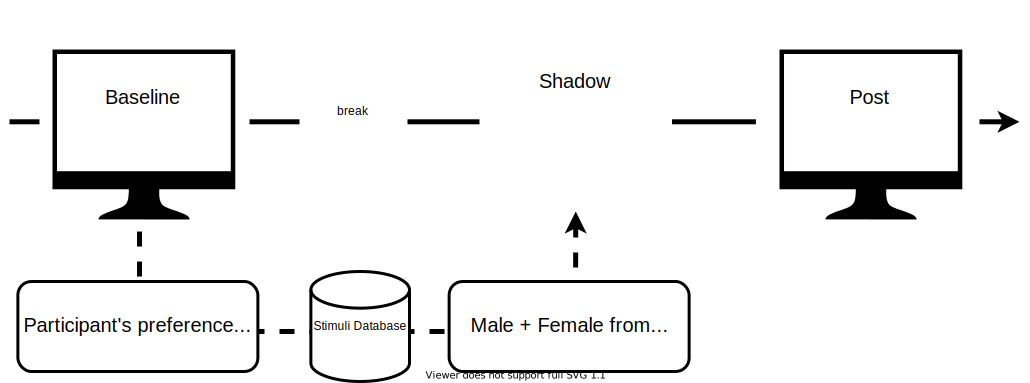
\includegraphics[width=\linewidth]{HCI_flow}
	\caption[\acs{hci} convergence experiment workflow]
		{Flow of the experiment (from left to right).
		Stimuli are read from a monitor in baseline and post phases, while heard over headphones in the shadowing task.
		The participant's preferred variation recorded in the baseline productions are used to select those with the opposite realizations from the stimuli database for the shadowing task.
		Each participant listened to both male and female voices of one of the stimulus types natural, diphone, or \acs{hmm}.}
	\label{fig:HCIConvFlow}
\end{figure}

\subsection{Analyses and results}
\label{subsec:results_hci}

The occurrences of each feature were analyzed separately.
The feature \textipa{[E:]} vs.\ \textipa{[e:]} was evaluated as a continuum in the F1-F2 formant space.
%Automatic annotations (WebMAUS, \cite{Kisler/etal:2017}) of all target vowel segments were manually corrected by a trained phonetician.
The first and second formants of each target segment were measured at the temporal midpoint in all productions as well as in the stimuli using Praat \citep{Boersma2018praat}. 
These values were used for calculating the Euclidean distance between the participants' and stimuli vowel realizations in each sentence using the formula
%
\begin{equation}
	E_{dist}=\sqrt{(F1_{participant}-F1_{model})^2+(F2_{participant}-F2_{model})^2}.
\end{equation}
\eqname{Euclidean distance in F1-F2 space}
\noindent
%
Smaller distance in the shadowing or post phases compared to the baseline phase points to a convergence effect.
\Cref{fig:ee_E_space} illustrates the convergence effects as realized by one of the participants.
The distances were measured using the mean values of all stimuli in the set to which the participant listened.
These distances were used to fit linear mixed-effects models with phase as fixed effect, subject and target word as random effects (intercepts and slopes), and distance as the dependent variable.
Models were fit for both preference groups compared by an ANOVA.
The differences between baseline and shadow phases were found to be significant in the natural and \ac{hmm} groups, and between the baseline and post phases only in the natural group.
\Cref{tab:lmm_ee_E} summarizes the results for this feature.
\todo[inline]{write a few sentences about the too-similar vowel in the synthetic sets and refer to figure.}
%
\begin{table}[t]
	\centering 
	\caption[Convergence results for \textipa{[E:]} vs.\ \textipa{[e:]} with three stimuli sets]
		{Summary of convergence effects between the three phases.} 
	\label{tab:lmm_ee_E} 
	\sisetup{table-format=3.2, parse-numbers=false}

	\begin{tabularx}{\linewidth}{XSSS}
		\toprule
		\textbf{Natural} & \multicolumn{1}{c}{\textbf{base-shadow}} & \multicolumn{1}{c}{\textbf{base-post}} & \multicolumn{1}{c}{\textbf{shadow-post}}\\
		\midrule
		intercept           & 69.94\textsuperscript{***}		& 32.88    	& $-$33.67\textsuperscript{**} \\
                         	& (14.89)  		& (17.53)  	& (11.44)     	\\
		\textsc{preference}	& 33.79\textsuperscript{*}		&          	&             	\\
                         	& (14.89)     	&          	&             	\\
 		\midrule
		observations 		& 210 			& 210 		& 209 			\\ 
		\bottomrule
	\end{tabularx}	

	\begin{tabularx}{\linewidth}{XSSS}
		\toprule
		\textbf{Diphone} & \multicolumn{1}{c}{\phantom{\textbf{base-shadow}}} &
        \multicolumn{1}{c}{\phantom{\textbf{base-post}}} &
        \multicolumn{1}{c}{\phantom{\textbf{shadow-post}}} \\
		\midrule
		intercept           & $-$1.68  	& $-$1.49  	& 0.44   \\
                        	& (8.72)   	& (9.93)   	& (7.24) \\
% 		\midrule
%		observations 		& 177 		& 179 		& 178    \\ 
		\bottomrule
	\end{tabularx}
	
	\begin{tabularx}{\linewidth}{XSSS}
		\toprule
		\textbf{\ac{hmm}} & \multicolumn{1}{c}{\phantom{\textbf{base-shadow}}} &
        \multicolumn{1}{c}{\phantom{\textbf{base-post}}} &
        \multicolumn{1}{c}{\phantom{\textbf{shadow-post}}} \\
		\midrule
		intercept      	& 32.64\textsuperscript{*} 	& $-$2.12  	& $-$31.23 \\
                       	& (13.61)  	&(12.38)  	& (15.86)  \\
% 		\midrule
%		observations 	& 134 		& 135 		& 133      \\ 
		\bottomrule
		\multicolumn{4}{l}{\small{$^{***}p<0.001$, $^{**}p<0.01$, $^*p<0.05$}}
	\end{tabularx} 
	\todo[inline]{numbers in table are not perfectly aligned because of parentheses}
\end{table} 
%
\begin{figure}[t]
	\centering
	\begin{minipage}{.47\linewidth}
		\centering
		\includegraphics[width=\linewidth]{ee_E_space}
		\caption[Example of vowel quality convergence towards a model speaker]
			{An example of a participant's vowel quality convergence towards the stimuli.
			The participant's preference is \textipa{[e:]} while the variation \textipa{[E:]} is used in the stimuli (and cf.\ \cref{fig:ee_E_circles}).
			The colors of the circles represent the {\color{base-green}\textbf{base}}, {\color{shadow-red}\textbf{shadow}}, and {\color{post-blue}\textbf{post}} phases, and the model's formant values with $\pm1$ standard deviation from the bivariate mean.
			The arrow shows the distance between one of the participant's production and the {\color{model-orange}\textbf{model mean}}.}
		\label{fig:ee_E_space}
	\end{minipage}
	\hfill
	\begin{minipage}{.47\linewidth}
		\centering
		\includegraphics[width=\linewidth]{ee_E_circles}
		\caption[F1 and F2 value areas of all stimulus groups]
			{Values areas of the first two formants of the three stimulus sets' \textipa{[e:]} and \textipa{[E:]} instances.
			 Each color represents both male and female ranges of on stimulus type (natural, diphone, or \ac{hmm}).
			 The smaller a circle is, the more well-defined the mean target of this stimulus group is.
			 Moreover, the further apart circles of the same color are, the more distinct the difference is within this set.}
		\label{fig:ee_E_circles}
	\end{minipage}	
\end{figure}

The \textipa{[I\c{c}]} vs.\ \textipa{[Ik]} was evaluated based on the percentage of same-category realizations of the participants with respect to the stimulus set they listened to.
If the percentage increased, e.g., between baseline and shadow productions, the participant converged to the stimuli.
\Cref{fig:ic_ik_results} summarizes the per-phase differences for each set.
With all three data sets combined, the number of same-variant productions increased by about \SI{30}{\percent} from the baseline phase to the shadowing phase, and decreases again in the post phase, but to a lesser degree.
That means that all in all, participants not only converged to the stimuli in the shadowing phase, but the effect lasted to some extent in the post phase as well.
The statistical significance between the phases within each stimulus type was tested using a Gaussian linear mixed-effects model.
For both the natural and diphone sets, the increases between the baseline and the shadowing phases were significant, \SI{10}{\percent} to \SI{39}{\percent} and (\SI{16}{\percent} to \SI{48}{\percent}, respectively.
Moreover, in these sets the decreases in the post phase did not go all the way to the baseline level: \SI{39}{\percent} to \SI{23}{\percent} for natural and \SI{48}{\percent} to \SI{36}{\percent} for diphone.
For the \ac{hmm} set, the increase between baseline and shadowing was \SI{8}{\percent} to \SI{40}{\percent} and did not reach the significance threshold.
However, the decrease in the post phase reached the baseline level again and was significant, from \SI{40}{\percent} to \SI{12}{\percent}.
%
\begin{figure}[t]
	\centering
	\includegraphics[width=\textwidth]{ic_ik_results}
	\caption[Convergence results for \textipa{[I\c{c}]} vs.\ \textipa{[Ik]} with three stimuli sets]
		{Percentage of same-variant and different-variant realization of participants with respect to the stimulus type they listened to in the shadowing phase.
		An increase between the base and the shadow phases indicates convergence towards the stimuli.
		Similarly, the decrease between the shadow and the post phases back towards the baseline level shows the degree to which the convergence effect remained when the stimuli were not present anymore.}
	\label{fig:ic_ik_results}
\end{figure}
%

The \textipa{[\s{n}]} vs.\ \textipa{[@n]} was measured based on the lengths of the potential schwa segments in the sentences.
To decide whether schwa was present or absent in the participants' target word productions, the lengths of relevant segments between the preceding consonant -- \textipa{[d], [t], [\c{c}], [x], or [f]} -- and the final nasal were measured.
A duration of \SI{30}{\milli\second} was established as the threshold of a perceived schwa segment.
This decision is also supported by the fact that all schwas occurrences in the stimuli sets were at least \SI{30}{\milli\second} long.
The segment length range of the natural stimuli along with the lengths variance of the participants' productions are shown in \cref{fig:schwa_conv_bars}.
Note that only two participants showed preference toward the \textipa{[@n]} variant in their baseline productions (cf.\ \cref{tab:preference_hci}).
This indicates that schwa does not commonly appear in the examined context, which might make it harder to trigger convergence among the participant.
Seeing that a statistical analysis for a groups of two participant is likely to be misleading, these participants were excluded from the analysis of this feature.
\Cref{tab:schwa_results} summarizes the percentage of schwa occurrences in the three phases.
There was an increase of schwa occurrences between the baseline and shadowing phases all stimulus types, with the difference being significant for the natural and \ac{hmm} sets with changes of \SI{9}{\percent} and \SI{5}{\percent}, respectively.
In the post production, the number of schwa occurrences decreased to approximately the baseline level for all conditions.
Interestingly, while for the natural stimuli this decrease was still above the baseline percentage, for both the synthetic sets the percentage in the post phase was even lower than in the baseline phase.
%
\begin{figure}[t]
	\begin{minipage}{.48\linewidth}
			\centering
			\includegraphics[width=\textwidth]{schwa-plot}
			\caption[Illustration]
				{Schwa segment lengths in the three phases.
				 The height of each bar represents the average length in this phase, and the corresponding whiskers indicate the overall value range.
				 The gray area shows the value range of the stimuli, with the mean length at the orange dashed line.}
			\label{fig:schwa_conv_bars}
	\end{minipage}
	\hfill
	\begin{minipage}{.49\linewidth}
			\centering
			\captionsetup{type=table}
			\caption[Convergence results for \textipa{[\s{n}]} vs.\ \textipa{[@n]} with three stimuli sets]
				{Percentage of schwa occurrences in each phase and stimulus set.
				 $N$ stands for the number of sentences with the target feature \textipa{[\s{n}]} vs.\ \textipa{[@n]}, which is derived from the number of participant with \textipa{[\s{n}]} preference (the shadowing phase always has double the number of sentences, because both male and female voices were used).}
			\label{tab:schwa_results}
			\begin{tabularx}{\linewidth}{lccc}
				\toprule
				& \textbf{base} & \textbf{shadow} & \textbf{post} \\
				\midrule
				\multirow{2}{1.4cm}{Natural}	& \SI{1.9}{\percent} & \SI{10.9}{\percent} & \SI{3.8}{\percent}  \\\vspace{0.3cm}
											& $ N = 105 $ 		 & $ N = 210 $		   & $ N = 105 $		 \\
				\multirow{2}{1.4cm}{Diphone} 	& \SI{2.4}{\percent} & \SI{4.1}{\percent}  & \SI{1.2}{\percent}  \\\vspace{0.3cm}
											& $ N = 85 $ 		 & $ N = 170 $ 		   & $ N = 85 $			 \\
				\multirow{2}{1.4cm}{\acs{hmm}} 	& \SI{2.5}{\percent} & \SI{7.5}{\percent}  & \SI{1.25}{\percent} \\
											& $ N = 80 $ 		 & $ N = 160 $ 		   & $ N = 80 $			 \\
				\bottomrule
			\end{tabularx}
	\end{minipage}
\end{figure}

\todo[inline]{for both studies, put Procedure between Target Features and Stimuli}

\section{Conclusion}
\label{sec:conclusion_shadowing}

The results found in the music experiment show that alignment occurs in singing, more so with respect to temporal features than to tonal ones.
This stands in contrast to findings in interactive speech \citep[e.g.,][]{Raveh2019InterspeechAlexa}).
Even so, the results emphasize the similarity between the two oral capabilities, viz.\ speech and singing, which are both used in human communication.
They are therefore also prone to influence each other and can potentially be related and enhance one another.
For example, \citet[][p.\ 216]{Nardo2009musicality} explain that \emph{tonal} and \emph{rhythmic} abilities are measures of musicality and also related to phonetic talent.
This idea is also supported by \citet{Tsang2018musical}, who found a correlation between musical experience and sensitivity to convergence.
Similarly, pitch has been found to correlate with the level of agreement between interlocutors in dyadic conversation \citep{Okada2012interpreting}.
We therefore suggest that speech and music are two domains where certain common effects, and in particular convergence, occur with respect to shared prosodic features.
Establishing this connection between music and speech offers a wide variety of further interdisciplinary experimentation that combine linguistic and musical analysis methods.
Specifically for convergence, the influence of listening to people with different social and vocal characteristics can be examined.
The manner in which distances in vocal behavior decrease, or increase, can depend on further aspects of the social environment and auditory context, as suggested by \citet{Noy1999psychoanalysis}.
To sum up, the first hypothesis -- convergence to perceived musical stimuli -- was satisfied, but not in the same way for pitch and tempo.
While tempo became globally closer to the recorded version in absolute terms, the tones were produced more precisely but within the same tonal range.
Additionally, the secondary expectation was only partially met, with fewer large deviations occurring in the shadowing performances, but otherwise the tones in the baseline production were slightly more accurate as a whole.
Finally, the third hypothesis was fulfilled, as the simpler, frequent rhythmic patterns were replicated more correctly.
Furthermore, with one exception, participants were not able to replicate the entire lullaby.
Interestingly, they remembered either part A or B, but didn't mix bars from both.

As for the \ac{hci} experiment, different degrees of convergence were found for each of the three target features.
The feature \textipa{[E:]} vs.\ \textipa{[e:]} showed convergence effect in all stimulus sets, but only in the natural set this effect was significant.
The areas covered by each vowel in \cref{fig:ee_E_circles} sheds light on possible reasons for the overall worse performance of the synthetic stimuli.
First, the vowels of the same category from the male and female diphone voices occupy a much larger area than those from the male and female natural voices, which results in a less distinct convergence target.
And second, all instances that are supposed to be \textipa{[E:]} in the female \ac{hmm} voice are located in the area of \textipa{[e:]}.
Hence, in the \ac{hmm} condition, all participants with preference \textipa{[e:]} actually heard their preferred version of the vowel in half of the trials during the shadowing phase.
These lead to the conclusion that the lack of a stronger effect could be due to the acoustic properties of the target vowels in the synthetic stimuli and not necessarily to the synthetic nature of the stimuli itself.
The feature \textipa{[I\c{c}]} vs.\ \textipa{[Ik]} was found to be a consistent trigger of phonetic convergence.
For all three stimulus types, the participants produced the opposite variant than their preference in roughly a third of the trials.
These cases of convergence do not only stem from participants that already showed both target forms in the baseline production, but also from participants that produced only one of the two forms in the baseline phase.
This a strong effect compared to the other two target features.
It might be explained by the fact that this feature is categorical by definition, as opposed to the other feature which have two defined categories but are realized on a continuum (formant values and segment length).
The feature \textipa{[\s{n}]} vs.\ \textipa{[@n]} showed a rather small convergence effect.
This was expected, as schwa is not usually produced in the word-final sequence \textit{-en}.
Nevertheless, in all three conditions more instances of schwa were produced during the shadowing phase than in the baseline and post phase.
These productions are mostly attributable to one or two participants per condition who responded even to this unusual segmental feature.
This leads us to observe that apart from the identified group differences, the overall degree of convergence varied considerably among the participants, with some being \enquote{resistant} to external influence and others responding strongly to them.
In conclusion, it can be summarized that humans do indeed converge phonetically when interacting with synthesized speech. 
However, the degree of convergence depends on the nature of the target feature.   
Perceptibility of the target feature in the stimuli is proposed as a possible explanation for the fact that one of the examined features did not show the same extent of convergence for the synthetic stimuli as for the natural ones.

The two shadowing studies presented here show that vocal accommodation can also be found in a controlled experimental environment as part of a quasi-conversational scenario.
As a continuation of the effects found in \cref{chap:conv_analysis}, these results demonstrate that vocal accommodation occurs also in non-speech and human-computer settings.
These -- and especially the latter -- prove that accommodation effects are not exclusive to \acp{hhi} and thus lay the foundations for further investigation in \ac{hci}.
In chapter \cref{chap:speech_variations_in_hhci}, accommodation toward a computer-based interlocutor is examined in conversational, goal-oriented tasks.
The great individual differences found in these experiments inspired part of the parameters and approaches used in \crefrange{chap:computational_model}{chap:statistical_model}.
Their importance lies in the ability to give different \enquote{characters} (or \emph{profiles}, see \cref{subsec:accommodation_levels}) based on different human behavior, rather than letting a system behave the same in every interaction.
Furthermore, showing that convergence can occur in segmental features as well emphasizes the importance of control over such properties in synthetic speech for triggering vocal accommodation, which is attributed mostly to \ac{hhi}.
The segmental manipulations demonstrated in \cref{subsec:speech_manipulation} show how such differences can be achieved.
\chapter{Accommodation in Multiparty Interaction with an Agent}
\label{chap:speech_variations_in_hhci}

\lettrine{M}{ore} dynamic vocal behaviors can be established in interactions with multiple interlocutors.
This is not only due to the additional possible connections between them, but also because of other factors that might influence them, like the order of speech or the role of each speaker.
A \acl{hhci} study is presented in this chapter, where the effects of different aspects and conditions on vocal accommodation are investigated.

\pagebreak

\acresetall

\section{Speech variations in human-human-computer interaction}
\label{sec:accommodation_in_multiparty_interaction_with_an_agent}

Nowadays, we are witnessing an ever-growing presence of devices with spoken interaction capabilities in our everyday lives.
As argued in \cref{subsec:personal_assistants}, the use of \acp{pa} is rapidly increasing, as more mundane tasks can be achieved using them.
The question arises, therefore, whether different speech patterns and characteristics emerge in such \ac{hci} compared to \ac{hhi}; and if yes, which.
%One way of measuring these differences is in terms of linguistic similarity between the interlocutors.
%It has been demonstrated that humans may change their speech behavior when interacting with computer-based systems.
%In various \ac{hci} experiments, participants have been found to speak differently to computers and change their speech during the interaction \citep[e.g.,][]{Branigan2010linguistic}.
The vast majority of experimental work done in the field of vocal accommodation deals with the smallest social interactions, namely dyadic conversations.
Those can be dyads of two human speakers in \ac{hhi}, or a human and some computer-based agent in \ac{hci}.
Vocal accommodation in these types of interactions is explored in \cref{chap:shadowing_in_sung_music_and_human_computer_interaction,chap:conv_analysis}.
However, social interactions may also consist of three or more participants.
This is true for both \ac{hhi} and \ac{hci}, but also for interactions with mixed human and computer-based interlocutors and specifically multiple humans talking with a single device.
The latter can occur in various situations, like a person consulting a \ac{va} regarding availability in a weekly schedule while setting an appointment with a colleague or two friends ordering tickets from a voice-activated machine.
Mixed multiparty interactions already take place in various real-world situations lives.
Their popularity -- and sometimes necessity -- increase alongside the rise in use of \ac{c-ai} devices, such as \acp{va}, voice-activated cars, hands-free medical assistants, \acp{its}, social robots, and others.
It is important, therefore, to understand whether convergence, divergence, and other effects (like those described in \cref{subsec:variation_types}) may occur not only in \acp{hci}, but in \acfp{hhci} as well.
Various \ac{hci} experiments have shown that participants speak differently to computers and change their speech behavior during the interaction \citep[e.g.,][]{Branigan2010linguistic}.
Some works also compared the reaction of participants to different configurations of the computer-based interlocutor \citep[e.g.,][]{Levitan2016implementing}.
Yet, none of those has performed a comparison between human-directed and computer-directed speech within a single multiparty interaction.
Moreover, only the influence of the system's speech output on the user speech is typically examined in accommodation experiments, but not the influence of another human interlocutor.

Empirical work on multiparty \ac{hci} includes experiment where participants interact with different types of agents, like social robots \citep{Foster2012two, Ibrahim2019fundamental} and human avatars in immersive virtual worlds \citep{Traum2002embodied}.
Even in dyadic form, spoken interactions are a hard task for computers.
All the more so, when more than one other interlocutors are involved.
Measuring accommodation becomes more complex with multiple interlocutors involved, as discussed in \citet{Rahimi2019acoustic}.
There are many technical challenges on the way to realistic, real-time interactions with computers, including -- but not limited to -- center-of-attention detection, active speaker detection, turn taking, understanding private and shared knowledge, and of course correct speech production and understanding.
Interactions with machines are challenging for humans, too, since the former do not behave and react the same way (and often speed) as humans.
An example of such a social activity that is reasonably easy for humans to learn but still far from being feasible by computers are social games with a large number of participants.
These games typically require the players to be deceptive, track and exploit the behaviors of others, and react quickly to ever-changing dynamics between the players.
\Citet{Jonel2018Farmi} describe the challenges of such scenarios and discusses way to cope with them.
The type and severity of those problems depend also on the type of the computer-based agent (see \cref{sec:types_of_sdss}).
For instance, embodied agents at least have some basic way to convey non-verbal information, whereas voice-only systems like \acp{va} do not.
On the one hand, this gives a wider range of expressions to embodied systems, but requires more communication channels to implement and coordinate on the other hand.

This chapter presents a study that examines interaction-level vocal accommodation in \ac{hhci}.
In this paradigm, two human speakers work collaboratively with an agent to complete tasks while only one of them can talk directly to the agent.
More details about the dataset and the tasks are given in \cref{sec:vacc}.
Investigating such a scenario contributes to the understanding of both the role of an agent in interactions with multiple humans and the influence of another human in a \ac{hhci}.
These two aspects are examined in the two \emph{components} of the study:
The \emph{addressee} component focuses on the differences between the participant's addressed interlocutor within a conversation \citep[][see]{Raveh2019ESSV}, and the \emph{crowd} component spotlights the influence of an additional human interlocutor on the participant's speech toward the agent \citep[see][]{Raveh2019InterspeechAlexa}.
The question tackled by the second component is whether and to what extent speaking to a second human interlocutor in the same interaction as the agent influences the accommodation toward it, i.e., whether users speak differently towards a \ac{va} when another human participates in the interaction.
to that end, the distributional and temporal analyses performed in \cref{sec:analysis_hhci} are based on the participants' \emph{speech directions}, i.e., \acf{hds} and \acf{dds}, as illustrated in \cref{fig:condition_comparison_addressee,fig:condition_comparison_crowd}.

\section[The \acl{vacc}]{Dataset}
\label{sec:vacc}

\begin{figure}[t]
	\centering
	\subfigure[Solo condition]
	{\raisebox{1.85cm}{\includegraphics[width=0.45\textwidth]{condition_solo}}
	\label{fig:condition_solo}}
	\hfill
	\subfigure[Confederate condition]
	{\includegraphics[width=0.45\textwidth]{condition_confederate}
	\label{fig:condition_confederate}}
	\caption[Solo and confederate conditions in \acs{hhci} setting]
		{Illustration of solo and confederate conditions.
		A black arrow represents direction of speech from speaker to addressee.
		Note that the confederate (in green) never talks or addressed by Alexa, but only the participant (blue).}
	\label{fig:conditions_comparison}
\end{figure}
%
The accommodations study presented here uses the \acf{vacc}\footnote{\url{http://www.iikt.ovgu.de/iesk/en/Research+Groups/MDS/Research/VACC-p-4624.html}}, introduced by \citet{Siegert2018VACC}.
This corpus is suitable for this study, because it comprises both \acp{hci} and \acp{hhci} with a 2\textsuperscript{nd} generation Amazon Echo Dot device using the default skill set and German female voice of the \acf{va} Alexa.
These configurations are referred to here as \emph{solo} and \emph{confederate} conditions, respectively.
\Cref{fig:conditions_comparison} illustrates the interlocutor relations in each condition.
Similar corpora were used to study automatic addressee detection \citep[e.g.,][]{Shriberg2013addressee, vanTurnhout2005identifying}.
Although the study here does not set addressee detection or classification as a goal, it aims to provide insights and accommodation-related measures that may be useful for such tasks.
In the \ac{vacc}, the male confederate was present in the room only during tasks in the confederate condition and always sat at the same location.
To simulate the spatial situation of a multi-party interaction with a \ac{va}, the participant and the confederate sat in similar distance from the device that was situated on a table, roughly forming an equilateral triangle \citep[see Figure 2 in][]{Siegert2018VACC}.
The participant had led the interactions with both the confederate and Alexa, and the confederate never talked to Alexa directly.
Therefore, in the confederate condition, the participant needed to alternately speak with the confederate and Alexa alternately as part of the same interaction, without explicitly signaling to whom each utterance is addressed.
%Two high-quality neckband microphones (Sennheiser HSP 2-EW-3) were used to capture the voices of the participant and the confederate speaker.
%Additionally a high-quality shotgun microphone (Sennheiser ME 66) captured the overall acoustics and the output of Amazon's Alexa.
Two tasks were performed in each condition:
In the calendar task, the participant's goal was to find available time slots for several hypothetical appointments with the confederate.
The participant's pre-defined calendar was stored on the device and was accessible only via inquiries to Alexa.
In the solo condition, the participants got written information about the confederate's availability, whereas in the confederate condition, the confederate could be asked about it.
The goal of the quiz task is to answer trivia questions, like \enquote{When was Albert Einstein born?}.
Since Alexa was not always able to immediately provide a full answer to all the questions, the required information could be gathered incrementally over multiple turns.
Here, the participant solved the quiz alone in the solo condition or teamed up with the confederate so that the two could discuss the question-asking strategy in the confederate conditions.
The calendar task was designed so that the way to its solution is relatively straightforward:
Query the device for possible times till a match is found.
This requires interacting mostly -- if not only -- with the computer-based interlocutor.
Indeed, this task typically elicited interactions, in which the participant interacted with the confederate or the device in discretely separate turn blocks in the confederate conditions.
\Ac{dds} blocks were, unsurprisingly, longer, as the confederate was only addressed when additional information about the task was required.
The quiz task's flow was more flexible, since the strategy as to which questions to ask Alexa can be determined by the participant, including the amount and frequency of the confederate's intervention in the confederate conditions.
Indeed, more dynamic alternations between \ac{hds} and \ac{dds} were observed in this task.
As a whole, the quiz task is less formal than the calendar task.

The dataset contains recordings of 27 (14 female) German native speakers in the age range of 20 to 32 years (mean 24~$\pm$3.3).
Each participant performed the quiz and calendar tasks in both solo and confederate conditions, for a total of 108 interactions (2 tasks $\times$ 2 conditions $\times$ 27 participants).
%An interaction was finished either by completing the task or by stopping it prematurely in case no further progress could be made, to avoid participant frustration.
%The latter, however, happened only a few times.
These interactions consist of approximately \num{13500} utterances, which were manually transcribed and annotated (speaker, speech times, addressee, etc.) and stretch over total recording time of \SI{17}{\hour} \SI{7}{\minute} (\SI{31}{\minute} average interaction length).
The permutations of the tasks, conditions, and their order were balanced.

%\begin{figure}[!h]
%	\begin{center}
%		\fbox{\parbox{6cm}{
%		This is a figure with a caption.}}
%		\includegraphics[scale=0.5]{image1.eps} 
%		\includegraphics[width=0.75\linewidth]{figures/IMG_4798.jpg}
%		\caption{A snapshot of the data collection setup. The confederate speaker (left side) and the participant (right side) are sitting around a table, where the voice assistant (Amazon Alexa Echo Dot) is located.}
%		\label{fig:wohnzimmer}
%	\end{center}
%\end{figure}


%The recordings were stored in WAV format with \SI{44.1}{\kilo\hertz} sample rate and 16 bit resolution.
%The recordings were manually separated into utterances, which were additionally annotated with its speaker, context, and textual transcription.
%The speaker of each utterance could be the participant, Alexa, or the confederate.
%The context marked the type of interaction of the utterance, which include \ac{hds}, \ac{dds}, cross-talk, off-talk, laughter, and more.
%To deal with clearer data, only \ac{hds} and \ac{dds} contexts were used for analysis in this paper.
%The transcription was obtained using the Google Cloud Speech API automatic speech recognition service.
%\cref{tab:dataset_charact} summarizes the dataset characteristics.

%\begin{table}[t]
%	% \captionsetup{format=plain,justification=raggedleft,width=.4\textwidth,hangindent=0pt,skip=500pt}
%	\centering
%	\caption{\ac{vacc} dataset characteristics}
%	\label{tab:dataset_charact}
%	\begin{tabular}{L{3cm}L{3cm}}
%		\toprule
%	     Participants 				& 27														\\
%	     Sex 						& Male 13 / Female 14 										\\
%	     Total Recorded Data 		& \SI{17}{\hour} \SI{7}{\minute}							\\
%	     Experiment Duration 		& Mean: 31 min 												\\
%		  Age (years)				& Mean 24 (Std: 3.32)										\\	% Min: 20; Max: 32  \\
%	     Language 					& German													\\
%	     Annotation 				& Transcription, Addressee, Laughter, Cross-Talk, Off-Talk	\\ 
%	     Supplementary self-reports & Evaluation of interaction, AttrakDiff, Speaking style, Experiences in interacting with voice assistants\\
%		\bottomrule
%	\end{tabular}
%\end{table}

\subsection*{Annotations}
\label{subsec:annotations_hhci}

Each utterance in an interaction was annotated with its speaker, context, and textual transcription.
The speaker of each utterance could be the participant, Alexa, or the confederate.
Cross-talk was rare, as the participants typically waited till the confederate or Alexa finished talking (except for when they tried to interrupt Alexa mid-utterance if the response was unquestionably wrong or irrelevant due to recognition error).
The context marks the utterance's interaction type, like \ac{hds}, \ac{dds}, cross-talk, off-talk, laughter, and more.
To deal with clearer data, only \ac{hds} and \ac{dds} contexts were used for analysis, which, together, constituted over \SI{90}{\percent} of the interactions' recording time.
Transcriptions were obtained using the Google Cloud Speech API automatic speech recognition service and were subsequently manually verified and corrected.
Utterances' start and end times were derived directly from the transcriptions' timestamps.

\section{Analysis}
\label{sec:analysis_hhci}

\begin{figure}[t]
	\centering
	\subfigure[\acs{hds} in confederate condition]
	{\includegraphics[width=0.45\textwidth]{condition_confederate_marked_hhi}
	\label{fig:condition_confederate_marked_hhi}}
	\hfill
	\subfigure[\acs{dds} in confederate condition]
	{\includegraphics[width=0.45\textwidth]{condition_confederate_marked_hci}
	\label{fig:condition_confederate_marked_hci}}
	\caption[\acs{hds} and \acs{dds} compared in confederate condition]
		{Illustration of the compared speech directions in the \emph{addressee component}.
		The orange arrows mark the compared speech directions (participant to confederate and participant to Alexa).}
	\label{fig:condition_comparison_addressee}
\end{figure}

\begin{figure}[t]
	\centering
	\subfigure[\acs{dds} in solo condition]
	{\raisebox{1.6cm}{\includegraphics[width=0.45\textwidth]{condition_solo_marked}}
	\label{fig:condition_solo_marked}}
	\hfill
	\subfigure[\acs{dds} in confederate condition]
	{\includegraphics[width=0.45\textwidth]{condition_confederate_marked_hci}
	\label{fig:condition_confederate_marked_hci_crowd}}
	\caption[\acs{dds} compared in solo and confederate conditions]
		{Illustration of the compared speech directions in the \emph{crowd component}.
		The orange arrows mark the compared speech directions (participant to Alexa with and without the presence of the confederate).}
	\label{fig:condition_comparison_crowd}
\end{figure}

A subset of the \ac{vacc} was used for the analysis in each component, which is suitable for the speech directions in question.
\Cref{fig:condition_comparison_addressee,fig:condition_comparison_crowd} illustrate the examined speech directions in each component.
Only the 54 interactions from the confederate conditions were used for the addressee component, as the alternations between \ac{hds} and \ac{dds} within an interaction were examined.
For the crowd component, all 108 interactions were taken, because the comparison required executions of the tasks performed in both solo and confederate conditions.
Interactions of all 27 participants were included in both subsets.
Despite the different sizes of the subsets, the number of comparisons was the same for both components, since the addressee component used both speech directions of the participants in each interaction (54 $\times$ 2 = 108) and the crowd component used only \ac{dds} but from both conditions (54 $\times$ 1 + 54 $\times$ 1 = 108).
These subsets were analyzed based on the audio signals and the annotations described in \cref{subsec:annotations_hhci}.
The speaker annotations were used to determine to which of the three speakers the measured values should be ascribed.
The text transcriptions were only used for verifying the correct audio segments were analyzed.
Comparisons were made between the utterances of the same interaction, i.e., within a single task.

To increase temporal resolution, the audio signals were cut into two-seconds \emph{slices}.
A single slice always contained audio from a turn of a single speaker.
Any remainder shorter than 2 seconds got a separate slice.
For example, a turn of length \SI{5.2}{\second} was sliced into three slices of \SI{2}{\second}, \SI{2}{\second}, and \SI{1.2}{\second}.
This way, values measured in a slice could belong only to one speaker.
Splitting the turns also creates equal, consecutive, and more comparable time units for an interaction without introducing artificial boundaries by dividing it into a pre-defined number of parts \citep[as in][]{Silber-Varod2018prosodic}.
This is especially important for the temporal analysis (\cref{subsec:temporal_analysis}).
Slice lengths of 0.5, 1, 5, and 10 seconds were experimented with as well.
However, those were proved too short to capture changes in \ac{ar} (see below), which is dependent on the size of this window, or two long for a comparable and uniform temporal resolution.
Two seconds was found to be a good compromise based on these criteria.

The following phonetic features were targeted: 
%
\begin{description}%[wide=0pt, leftmargin=0.5\parindent, nosep]
	\item[\Acf{f0}] -- mean pitch measured within a slice with hop size of \SI{100}{\milli\second} and a pre-defined range of \SIrange{60}{350}{\hertz}.
	\citet{Gregory1993Voice} found that this feature is used to produce social similitude and cohesiveness in dyadic interviews.
	Moreover, this feature showed convergence effects in an auditory naming task \citep{Babel2012role} and a \ac{hci} shadowing task \citep{Bulatov2009effect}.
	
	\item[Intensity] -- mean intensity measured within a slice with hop size of \SI{100}{\milli\second}.
	This feature showed significant entrainment effects in game scenarios \citep{Levitan2011measuring} and as a indicator for social desirability \citep{Natale1975convergence}.
	
	\item[\Acf{ar}] -- the ratio of number of syllables to phonation time within a slice, as described in \citet{DeJong2009arcitulcationrate}.
	\citet{Schweitzer2013convergence} examined this feature in the context of phonetic convergence, but no effect was found on turn-level and interaction-level analyses.
\end{description}
%
All features were measured individually in each slice automatically using Praat \citep{Boersma2018praat} scripts.
The preprocessing and analysis were performed using the system introduced in \citet[][and see \cref{chap:web-based_responsive_spoken_dialogue_system}]{Raveh2018Specom}.

\section{Results}
\label{sec:results_hhci}

Two analyses were carried out: distributional and temporal.
The first looks at global differences on the interaction level of the participants' productions.
The second examines time-based, continuous changes in the similarity between the participants and the other interlocutors.

\subsection{Distributional analysis}
\label{subsec:distributional_analysis}

\begin{table}[b]
	\centering
	\caption[Percentage of significantly different interaction pairs in crowd component]
		{Percentages of interactions in which the distributional difference of each feature was significant}
	\label{tab:results_hhci_addressee}
	\begin{tabularx}{\linewidth}{XSSS}
		\toprule
		& \acs{f0} 						& {intensity}				& \acs{ar}									\\
		signif.\ diff.					& \SI{74}{\percent}			& \SI{89}{\percent}		& \SI{13}{\percent} \\
		\acs{hds} mean (standard deviation) 		& 10.5\,\si{\hertz}			& 2.95\,\si{\decibel}	& 0.627				\\
		\acs{dds} mean (standard deviation) 		& 10 \,\si{\hertz}		& 2.61\,\si{\decibel}	& 0.634				\\
		\bottomrule	
	\end{tabularx}
\end{table}
%
The means, medians, and standard deviations of the target features in the participants' speech in each of the interactions were calculated for both \ac{hds} and \ac{dds}.
These measures shed light on the overall range of values used when the participant was talking to each of the other two interlocutors.
They were listed for each target feature chronologically throughout the interaction.
These lists were divided into four speech directions based on speaker and context:
the participant talking to the confederate, the participant talking to Alexa, the confederate talking to the participant, and Alexa talking to the participant (see four arrows in \cref{fig:condition_confederate}).
The contrast between \ac{hds} and \ac{dds} is observable within the participant's speech only, which was active in both contexts.
To detect these differences, the distribution of their respective values in the solo and confederate conditions in each interaction pair were compared.
This was done by using the two-sample Wilcoxon test \citep{Wilcoxon1945individual}, with $\alpha = 0.05$ with the null hypothesis that similar distributions of the target feature were used in both conditions.
A significant result of the test means that the participant produced the respective feature differently when interacting with Alexa alone compared to when the confederate participated as well.
\cref{tab:results_hhci_addressee} shows the percentage of interaction pairs, in which the null hypothesis was rejected, i.e., that the feature was utilized differently by the participant in each condition.

\begin{figure}
	\centering
	\includegraphics[width=.9\linewidth]{20171127A_Quiz_01_pitch_dist_cut}
	\includegraphics[width=.9\linewidth]{20171127C_Calendar_02_pitch_dist_cut}
	\vspace{0.3cm}
	\caption[Interactions with significant and insignificant \acs{f0} distribution]
		{Examples of \ac{f0} distributions in \ac{hds} and \ac{dds} with a \emph{significant} difference (top; quiz task of participant 20171127A; p~$\ll$~0.0001,~$\alpha=0.05$) and \emph{insignificant} difference (bottom; calendar task of participant 20171127C; p~=~0.71,~$\alpha=0.05$).
		The colors represent distributions of the participant (blue), Alexa (red), and the confederate (green).
		The line style differentiates between \ac{hds} (dashed line) and \ac{dds} (solid line).}
	\label{fig:hds_dds_dist}
\end{figure}
%
\begin{figure}
	\includegraphics[width=.85\linewidth]{20171127A_Quiz_01_intensity_violin_cut}
	\includegraphics[width=.85\linewidth]{20171127C_Calendar_02_intensity_violin_cut}
	\caption[Interactions with significant and insignificant intensity differences]
		{Examples of intensity distributions in \ac{hds} and \ac{dds} with a \emph{significant} difference (top; quiz task of participant 20171127A; p~$\ll$~0.0001, $\alpha=0.05$) and \emph{insignificant} difference (bottom; calendar task of participant 20171127C; p~=~0.55, $\alpha=0.05$).
		The colors represent distributions of the participant (blue), Alexa (red), and the confederate (green).
		The widths of a boxes represent the value frequencies and the \enquote*{+} sign marks their respective means.}
	\label{fig:hds_dds_violin}
\end{figure}

\Cref{fig:hds_dds_dist} show examples of the distributions of a participant's \ac{f0} in \ac{hds} and \ac{dds} contexts in the addressee component.
Since a female voice was always used for Alexa and the confederate was always male, there is a natural gap between their \ac{f0} values.
This gap leaves room for convergence to occur, i.e., change in the participants' production in the direction one of the other interlocutors.
As \cref{tab:results_hhci_addressee} shows, in \SI{74}{\percent} of the cases out of the 54 analyzed interactions the difference of the participant's \ac{f0} between \ac{hds} and \ac{dds} was significant.
Out of those, in \SI{85}{\percent} of the cases the distribution mass of \ac{dds} contained higher values than \ac{hds}'s, which indicates accommodation towards Alexa.
Unlike \ac{f0}, absolute intensity values may not be as meaningful due to the device's and the confederate's location relative to the participant's microphone.
This means that the absolute values of the participant's intensity in \ac{hds} and \ac{dds} can be compared directly, but only relatively against Alexa's and the confederate's.
Therefore, the differences of this feature as shown in \cref{fig:hds_dds_violin} should only be compared between the participant's both speech direction within an interaction.
These differences between the participants' \ac{hds} and \ac{dds} were significant in \SI{89}{\percent} of the cases.
In general, participants tended to speak to Alexa with a louder voice than to the confederate, although their distance from the participants was the same.
The differences between \ac{ar} distributions in \ac{hds} and \ac{dds} were significant in \SI{13}{\percent} of the cases.
This shows that the participants largely spoke with the confederate at the same speed as with Alexa.
Interestingly, the \ac{ar} was temporarily considerably lower when the participants tried to improve intelligibility, especially if the system's output indicated that it did not correctly understood the participant's utterance due to a recognition error.
%
\begin{table}
	\centering
	\caption[Percentage of significantly different interaction pairs in addressee component]
		{Percentage of interaction pairs with significant differences with respect to each target feature with all the interactions together and separated by order tasks.}
	\label{tab:signif_conditions}
	\sisetup{table-format=3.0}
	\begin{tabularx}{\linewidth}{XSSS}
		\toprule
		\thead[l]{feature} & {\thead{any order}} & {\thead{solo first}}	& {\thead{confederate first}}\\
		\midrule
		\acs{f0}	& 67	& 72	& 60 \\
		intensity 	& 67	& 76	& 56 \\
		\acs{ar}	& 30	& 31	& 28 \\
		\bottomrule	
	\end{tabularx}
\end{table}
%
In the confederate component, the performed each task both alone and with the confederate.
Since chronologically, by design, one of the conditions needed to precede the other, the percentages were also calculated separately for the cases where tasks were performed first in the solo condition and then in the confederate condition, and vice versa.
This separation shows whether interacting first with Alexa alone, without any human input, influenced the vocal behavior of the participants.
As there were no breaks between the components, the only factors for change were the order of the conditions and the involvement of another human speaker.
As shown in \cref{tab:signif_conditions}, the percentages of significant differences when interacting first only with Alexa were indeed higher by \SI{12}{\percent}, \SI{20}{\percent}, and \SI{3}{\percent} for \ac{f0}, intensity, and \ac{ar}, respectively.
\cref{fig:signif_cases_ordered} further breaks down the differences between interaction pairs and introduces the factor of the performed task.
In line with the tendency shown in \cref{tab:results_hhci_addressee}, the features \ac{f0} and intensity have the highest percentages of significant cases, regardless of the performed task, and the tasks performed first show higher percentages of different distributions.
In the lower percentages, it is the task, rather than the target feature, that shows differences between the cases.
And last, for \ac{ar}, with the lowest percentages, there is a clear difference between the quiz and the calendar tasks.
All in all, the \texttt{task} factor was a good indicator only for the feature with the lowest difference percentage and the \texttt{order} factor was more informative for the features with higher percentages.
To sum up, these results show significant differences in the majority of the cases for two of the three features for both the addressee and crowd components.
These outcomes provide a look into further aspects of \ac{hds} and \ac{dds} and speech-related features in \ac{hhci}, which may help studies in topics like addressee detection or vocal accommodation in  multiparty interactions.
%
%
\begin{figure}[t]
	\centering
	\includegraphics[width=.9\linewidth]{barplot_signif_cases}
	\caption[Per-case comparisons of distributional differences in the crowd component]
		{Percentages of cases with a significant difference between a feature's distributions in the solo and confederate conditions.
		A case is a combination of the factors \texttt{task}, \texttt{feature}, and \texttt{order}.
		For example, the case \texttt{Q.intensity.2} contains the comparisons of intensity in interactions of the quiz task where solo condition was performed second.}
	\label{fig:signif_cases_ordered}
\end{figure}

\subsection{Temporal analysis}
\label{subsec:temporal_analysis}

Looking at the distributional differences of the target features in \ac{hds} and \ac{dds} sheds light on the general speech behaviors of the participants.
However, this analysis leaves out an important aspect of spoken interactions, namely the time dimension.
While the interaction-level distribution measures show accommodation effects based on te overall range and frequency of a feature's values, the temporal analysis adds the information as to how they changed over time.
Adding the time dimension gives an overview of an interaction's structure and reveals additional insights regarding its dynamics, such as turn lengths, turn switching, pauses, and accommodation effects.
For that, trend lines for the temporal changes needs to be calculated.
This was achieved by smoothing the measured value using \ac{loess} \citep{Cleveland1988locally}, a non-parametric regression method that deterministically fits a function to a localized subset of the data.
The fitting was done for each speaker separately over all slices of \ac{hds} and \ac{dds} with measured values of the features.
The first plot in \cref{fig:hds_dds_time} shows a case where the absolute \ac{f0} values are roughly the same in \ac{hds} and \ac{dds}, but the participant's change patterns are different.
In the \ac{dds} context, the participant generally keeps a stable distance from Alexa's voice, whereas in the \ac{hds} context the \ac{f0} values gradually get closer to the confederate's.
In both contexts, the participant's \ac{f0} starts around \SI{150}{\hertz}, but in \ac{hds} the minimum \ac{f0} is only slightly below this initial value, whereas in \ac{dds} it drops as far as \SI{25}{\hertz} lower.
A similar example is shown in the second plot in \cref{fig:hds_dds_time} for the intensity feature.
Unlike the previous example, here the absolute values between \ac{hds} and \ac{dds} steadily differ by about \SI{5}{\decibel} (matching the tendency to talk louder toward Alexa, as described above), but the overall change is similar.
That is, in both cases the intensity rises from the beginning to around a quarter of the interaction's duration, and then decreases again until the end, in \ac{hds} more quickly than in \ac{dds}, down to approximately the same value as at the beginning.
Since \cref{fig:hds_dds_time} shows two examples of the quiz task performed by two different participants, it is possible to compare the structure of these interactions as well.
As described in \cref{sec:vacc}, the quiz task in the confederate condition is designed so that the two human speakers need to find an efficient way to solve the questions using Alexa.
After improving their strategy, the lead should ultimately be taken by the participant, who interacts with Alexa to solve the questions as quickly and correctly as possible.
In both examples, the first half of the interaction contains relatively short turns and rapid addressee changes.
This might be ascribed to the fact that the participants are still trying to figure out the best way to interact with Alexa and the confederate.
Then, sometime after the middle of the interaction, there is a larger block of \ac{dds}, followed by some more turns of \ac{hds} where the participants discuss with the confederate about ways to solve the remaining questions.
Finally, the interactions end with a shorter block of \ac{dds}, in which the participants finish these last questions of the quiz.
This structure quiz task was found in most participants' performances.
%
\begin{figure}
	\vspace{-0.8cm}
	\centering
	\includegraphics[width=.88\linewidth]{20171129A_Quiz_01_pitch_time_cut}
	\includegraphics[width=.88\linewidth]{20171129B_Quiz_02_intensity_time_cut}
	\caption[Temporal comparison of \acs{f0} and intensity trends in \acs{hds} and \acs{dds}]
		{The changes of \acs{f0} (top; quiz task of participant 20171129A) and intensity (bottom; quiz task of participant 20171129B) over time in \ac{dds} and \ac{hds} (upper and lower parts of each plot, respectively).
		Alexa's voice is marked in red, the confederate in green, and the participant in blue.
		The timespans on the x-axis are represented by turn slices, as explained in \cref{sec:analysis_hhci}, and the y-axis shows the values of the feature.
		A slice's background color indicates the speaker in this slice and the dots with the same color show the measured value of the feature in that slice.
		The trend lines are smoothed values calculated by LOESS \citep{Cleveland1988locally}.}
	\label{fig:hds_dds_time}
\end{figure}

%Another way to look at accommodation in an interaction is in the temporal dimension.
%In this analysis, the same raw measured values were used to examine changes that occur over time.
%That is, unlike the analysis presented in \cref{subsec:distributional_analysis}, here the order of the values (i.e., their change over time) plays a major role, and effects may be found in specific time windows.
%To perform such an analysis over the entire interaction, two additional computation steps are required.
%First, each point in time must have a corresponding value for each feature produced by all speakers.

%This results in a predicted value for each slice of the conversation.
The accommodation in each conversation were further examined by measuring the contribution of the participant to the overall mutual change.
\cref{fig:condition_convergence_comparison} illustrated a comparison of a participant's changes in the solo and confederate conditions.
The lower part of each plot shows the accommodation changes of the participant during the interaction (blue for convergence and red for divergence), and the upper part shows the floor changes.
Note that the confederate condition has fewer floor changes, because the analysis concentrates on the participant and Alexa, and the confederate turns are not shown.
The relationship between a feature's values in each slice needs to be determined to describe their temporal changes.
To investigate the accommodation effects, a measure for the relative change between slices was used, which calculates the participant's contribution to the overall change in proximity between the participant and Alexa.
Alexa's contribution is considered to be a static effect, as it is not deliberately changing its output based on the participant's speech.%, and is therefore not taken into account.
The degree of change between two slices is calculated by
%
\begin{equation}
	\label{eq:change}
	change_t = -\Delta_{t, t-1} \mid S_{part} - S_{Alexa} \mid,
\end{equation}
\eqname{Smoothed mutual change of two interlocutors}\noindent
%
where the index $t$ refers to the current slice and $S_{part}$ and $S_{Alexa}$ are the smoothed values of the participant and Alexa, respectively.
The minus sign at the front flips the value so that convergence is represented by positive values and divergence by negative values.
Subsequently, the participant's contribution toward the accommodation is calculated by
%
\begin{equation}
	\label{eq:accommodation}
	accomm(participant)_t = change_t - \Delta_{t, t-1} S_{Alexa}.
\end{equation}
\eqname{Speaker's contribution to accommodation}\noindent
%
%
\begin{figure*}[t]
	\centering
	\includegraphics[width=\linewidth]{20171127B_Quiz_pitch}
	\caption[Temporal comparison of accommodation in solo and confederate conditions]
		{A comparison between \ac{f0} changes in solo (left) and confederate (right) conditions.
		The horizontal lines show the smoothed trends of the participant (blue) and Alexa (red).
		Confederate turns and omitted segments (as per \cref{subsec:annotations_hhci}), are not colored (gray).
		The vertical bars in the upper halves represent the turns of the participant (blue) and Alexa (red).
		The color-scaled vertical bars at the bottom halves show the convergence (blue) or divergence (red) level of the participant as calculated by \cref{eq:accommodation}.
		The darker the color, the greater the effect, with white indicating no change (or synchrony, in segments with both trends moving the same way).}
	\label{fig:condition_convergence_comparison}
\end{figure*}
%
The sum of the changes of each target feature produced by all participants in every interaction (i.e., a sex-task-condition-order combination) was calculated, resulting in a single value that represents the overall change per feature.
A value greater than zero means that more convergence was observed, while a negative value points to more divergence.
There were only two instances where this value was exactly zero, both for the \ac{ar} feature.
These instances were treated as cases of divergence, for their divergence spans were longer.
Using this approach, only a few interactions had no feature convergence in them, and several had all three features showing convergence.
However, a stricter threshold was applied, where a feature was considered as converging only if its overall accommodation value was higher than one standard deviation from its mean.
Based on this criterion, all interactions were categorized by the number of features that showed more convergence in them.
\Cref{fig:alluvial} summarizes this categorization for each factor.
Each line represents a single interaction, and the strata it goes through form the factor combination of this interaction.
The number of features that showed more convergence than divergence overall is marked by the color of the line.
Some tendencies emerge from this categorization:
first, in \SI{35}{\percent} of the interactions, there was at least one feature that showed convergence, but in none of them did so all three features (though there were such cases with the more tolerant criterion).
In seven interactions, two features showed convergence, two of which by male participants and five by females.
In total, males converged in \SI{5}{\percent} of all measurements and females in \SI{7}{\percent}.
Furthermore, of all converged features, \SI{58}{\percent} occurred in the solo condition, compared to \SI{42}{\percent} in the confederate condition.
However, no substantial difference between the calendar and quiz tasks was found, with \SI{49}{\percent} and \SI{51}{\percent} of the cases, respectively.
The same holds for the comparison between the two orders in which the tasks could be performed.
These results support the addition of the confederate to the interaction as the factor for less convergence occurring in interactions.
%
\begin{figure}[!t]
	\vspace{-0.5cm}
	\centering
	\includegraphics[width=.9\linewidth]{alluvial_4factors_numConv_strict}
	\caption[Number of features showing convergence categorized by factor]
		{Overview of the relation between the factors \texttt{sex}, \texttt{condition}, \texttt{task}, and \texttt{order} and the number of features that showed more convergence in total across all interactions.
		Each line represents one interaction.
		% The \texttt{sex} stratus refers to the sex of the participant, and the \texttt{order} stratus to the position of an interaction in the order in which the task-condition combination was performed.
		The line colors stand for the number of target features that showed overall convergence in this interaction, from none (zero features, in gray), through one (red), and up to two (blue).
		%		and up to all three features (green).
		For example, a blue line going through the strata sequence \emph{female $\rightarrow$ solo $\rightarrow$ quiz $\rightarrow$ first} represents an interaction with a female participant performing the quiz task in solo condition first, in which the participant converged in two out of the three target features.}
	\label{fig:alluvial}
\end{figure}
%
\section{Conclusion}
\label{sec:discussion_hhci}

The study in this chapter investigated vocal accommodation in \acf{hhci}.
\emph{Addressee} and \emph{crowd} components of the study examined different aspects of simulated real-world use cases, in which a human user talks alternately with a computer-based interlocutor and another human interlocutor.
The addressee component looked at differences between \acf{hds} and \acf{dds} within an interaction, while the crowd component focused on differences in \ac{dds} with and without the presence of the other human speaker.
Distributional and temporal accommodation analyses were performed in both components to provide interaction-level and time-related insights.

Three features were analyzed in the study: \acf{f0}, intensity, and \acf{ar}.
The first two features show a greater degree of difference in both components than the third.
Furthermore the changes were even greater in the crowd component, in which a human interlocutor was involved.
This indicates that not only \ac{f0} and intensity are more prone to variation than \ac{ar} in general, but also that human interlocutors trigger these variations more.
There several possible reasons for this difference.
First, computer-based agents, such as Amazon Alexa used here, do not change their speech output in any way, regardless of variations in the user's speech input.
As a social, mutual process, accommodation is more likely to be stronger if both interlocutors contribute to the overall effect.
In this study, the process can only be mutual in \ac{hds}, where another human is involved.
Nevertheless, accommodation indeed occurred in \ac{dds} as well, both with and without the presence of the confederate.
Secondly, due to this spontaneous nature of accommodation in \ac{hhi}, the participants might have automatically spoken more dynamically toward the confederate, due to the inherently expected dynamic variations is in human interlocutor.
Finally, \acp{va} (and voice-activated devices as a whole) are, in for the most part, still not performing well enough for people to speak to them as fluently and naturally as with humans.
This results in a different manner of talking to machines.
For example, users are more likely to articulate whole sentences, typically without reformulating, when requested to repeat their utterance by the device, whereas human interlocutors are capable of requesting and conveying corrections with shorter segments using intonation and other means.
Furthermore, although generally more seldom vary, users tend to reduce their \ac{ar} when repeating their utterances to the device, or when trying to be more clear.
This resembles the way people talk to children when they want to be more clear.
However, due to the way \ac{asr} systems are trained, more often than not this achieves the opposite result.
While participant did not change their \ac{ar} much toward Alexa, they did show accommodation in \ac{f0}.
This can be explained by the natural difference in male and female \ac{f0} ranges, which leaves room for accommodation for participants of both sexes (Alexa used a female voice while the confederate was always male).
In that case, the results shown here point to the fact that the participants generally treated Alexa as a human interlocutor with regards to \ac{f0} behavior, as opposed to talking to Alexa using a more monotonous \ac{f0}.
This happened despite Alexa not varying her \ac{f0} beyond the sentence-level intonation.
A similar effect was found for intensity.
Since the device and the confederate were squally distanced from the participants, there was no apparent reason for the participants to speak more loudly with either interlocutor.
Therefore, an explanation of the tendency to speak more loudly to the device may come from the intuition that a computer-based system has a harder time understanding human speech and therefore needs a clearer signal (also using lower \ac{ar}, as explained above).
This stands in line with the interpretation that humans sometimes treat voice-activated devices as humans who need a hyper-articulated speech signal to understand, like toddlers or language learners\footnote{In a sense, this analogy is correct, as the devices -- or rather their \ac{asr} components -- indeed learn to process speech signals.
Despite that, this process is different than the way babies acquire spoken language, and therefore such projection on the speech style does not help the device improving its understanding of the user.
Moreover, slower or disfluent speech may actually hinder the systems' understanding, as they are typically not trained on this kind of speech.}.
Another explanation may be the illusion that Alexa feels more distant than the human interlocutor because she is not an embodied agent \citep[cf.][and see \cref{sec:types_of_sdss} for further details]{Staum2010virtually, Gijssels2016speech}.
Keeping in mind that humans strive to communicate as efficiently as possible, it seems like changing these features helped the participants -- or at least felt like they did -- to interact better with Alexa.
Regardless of whether this roots from the unconscious attempt to treat the device as a social actor in the conversation \citep{Nass1994computers, Nass2000machines} or the fact that accommodation occurs, even if to a lesser extent, even when it's not mutual, the effect still took place.
This is, however, not the case with \ac{ar}, which shows a lower percentage of significant differences.
This indicates that \ac{ar} does not tend to vary as much as \ac{f0} and intensity, which stands in line with other studies, like \citet{Schweitzer2013convergence}.
Slower, more carefully articulated speech, occurs less often in regular speech than louder speech or higher pitch.
Such enhanced articulation not only takes longer to produce, but also requires more effort, making it a less preferred way to communicate, unless necessary.
In this somewhat formal experimental setting, participants are likely to speak more slowly than usual, and the motivation to complete the task in a short time encourages them not to speak even more slowly.
This supports the hypothesis that extra slow speech would only be used when necessary, e.g., when a repetition is required due to a recognition error on the system's side.
Once the misunderstanding was resolved, participants' went back to their original \ac{ar}.
These local changes may suggest that changes in \ac{ar} are done more consciously than in other phonetic features.

The results presented in \cref{tab:results_hhci_addressee,tab:signif_conditions} show that for all three features
\begin{enumerate*}[(a)]
	\item the distributions differed more when the participants first interacted with the device alone, and
	\item more convergence was aggregated in the task that was performed first.
\end{enumerate*}
This demonstrates the influences of the \texttt{order} factor.
Furthermore, the factors \texttt{sex} and \texttt{task} indicate that female participants showed a slightly higher amount of convergence in total than male participants, and that the performed task did not play role the increase or decrease of convergence.
The first speech input a participant encounters may cause a priming effect that, together with the natural tendency to converge to an interlocutor, results in a greater change in interactions that occur first.
However, the interchangeability of input (here, both \ac{hhi} and \ac{hci}) seems to hinder the ability of the participants to converge to Alexa.
One explanation for this may be that it is more natural for humans to accommodate to other humans, so once another human is involved, the accommodation towards the computer-based interlocutor is annulled.
Another possible explanation is that due to the multiple interlocutors, the participants do not have a steady target to accommodate toward, which leads to a weakened convergence effect.
This is confirmed by the higher number of convergence instances in the solo condition compared to the confederate condition in both the temporal and distributional analyses.
This could be explained as a reaction to a more stable vocal target (especially since Alexa generally doesn't change her voice much) than when alternating between two interlocutors.
Since \ac{hci} still lacks the mutuality of accommodation effects, the question arises whether these tendencies would be stronger in interactions with a single human versus interactions with two human speakers simultaneously.
The higher number of convergence instances by female participants may be ascribed to the \ac{va} using a voice of the same sex and could be further investigated by using a \ac{va} with a male voice.

%In conclusion, it is clear that accommodation effects and tendencies were present in both conditions, which is reassuring for future multiparty \ac{hci} accommodation research.
%Two main open questions remain concerning the temporal aspect of interactions.
%The first has do to with analysis on the speech \emph{signal level}, where the changes in measures over time can capture phenomena like convergence or divergence.
%In a more comprehensive analysis in this direction, more detailed patterns may emerge.
%Such an analysis can concentrate on one context or on comparing patterns in both \ac{hds} and \ac{dds}.
%Additionally, more features can be measured to reveal more details regarding speech behavior.
%The second may highlight behavioral patterns of the conversation on the \emph{turn levels}.
%This can include a closer examination of the interaction structure as a whole, the dynamics of turn changes, pauses and repetitions, etc.
%Such an analysis can be performed on interactions in solo and confederate condition to inspect whether humans deal with the same task performed with a computer alone differently than when another human is involved.

\part{Modeling}
\label{part:modeling}

\chapter[Computational Model]{Computational Model}
\label{chap:computational_model}

\lettrine{F}{or} a computer to express accommodative speech, a machine-understandable description of the process is required.
This chapter introduces a model of the way accommodation occurs in human speech, represented as a pipeline.
Its steps' order and logic are motivated by observed empirical data and aim to resemble the process that occurs in humans.
The parameters used in the pipeline to shape vocal behaviors are explained as well.

\pagebreak

\section{From \acs{hhi} to \acs{hci}}
\label{sec:from_hhi_to_hci}

The experiments presented in \cref{part:experiments} show humans' accommodation behaviors in different \ac{hhi} and \ac{hci} settings.
Complementary to that, \cref{subsec:accommodation_levels} discusses ways to represent the various levels of accommodative behaviors in computers.
Since behavioral changes, as explained by \ac{cat} (see \cref{sec:communication_accommodation_theory}), happen naturally and often unconsciously in \ac{hhi}, it is not trivial to transfer them to computers, as they need defined rules and numeric representation to process.
Numeric values can be achieved by applying some measuring technique appropriate for each feature, like formant values for vowel quality or frequency for \ac{f0}.
Rules for different behaviors, however, cannot be directly constructed, due to the intuitive nature of this inherent phenomenon, but can instead be inferred from observed \ac{hhi} data.
For example, the results of the study described in \cref{chap:shadowing_in_sung_music_and_human_computer_interaction} reveal a high degree of variation across participants (\cref{subsec:results_hci}).
While this is expected, further examination of these variations uncovers some general properties that can be taken as a basis for characterizing the different changes.
The link between the measured raw values and systematic rules should be a machine-applicable equivalence of the accommodation process in humans.
Such parallelisms would need to model, for instance, the way humans percept the accommodation-prone sounds, how they interact with previous instances and the current internal state of the sound in question, and the cognitive process of the phonetic changes.
Therefore, such a model should include the perception of the phonetic features, representation of the state change of each feature in memory, and the realization of the changes during a conversation.
Since these steps are, dependent on each other, the computational model presented here is depicted as a pipeline, where each of its steps stands for one of the sub-actions mentioned above.

\section{Pipeline representation}
\label{sec:pipeline_representation}

As accommodation happens automatically and seamlessly in human interlocutors' cognition, it is hard to say what are the exact steps this process comprises.
Some key properties stand out when examining many occurrences in different interactions.
The pipeline presented here aims to capture these properties and offer a defined process of describing the changes.
The advantages of representing this process as a pipeline (as opposed to, e.g., a one-step, end-to-end conversion) is that each facet of the process can be interpreted and controlled separately (ass demonstrated in \cref{subsec:computational_model,fig:adaptation_module_pipeline}).
This enables combining and experimenting with different methods and implementations for each step while maintaining their independence of each other.
The ability to substitute a single step's logic without influencing ther others grants the freedom to experiment with different methods without losing the core principles of the accommodation process.
For example, the calculation method in the \textit{update} step can be changed or even replaced by a statistical model (as the one in \cref{chap:statistical_model}).
Note that although only speech-related features are discussed here, this pipeline could be used for describing changes in other types of features and modalities that can be translated to numeric representations, like lexical choices, linguistic complexity, eye gaze, emotional state, etc.

The proposed pipeline representation consists of the following five main steps, which are explained in detail in \crefrange{subsec:detect}{subsec:assign}:
%
\begin{itemize}[topsep=0cm, itemsep=-.1cm, wide=0cm, leftmargin=!, labelwidth=\widthof{\textbf{update}}]
	\item[\textbf{detect}] hear and identify a feature that can be changed, corresponding to a human ear's ability to notice such variations;
	
	\item[\textbf{filter}] decide whether the encountered feature's instance appears in a way that can trigger change, capturing the inherent detection of phonological context and rules in the language;
	
	\item[\textbf{store}] add the instance to the exemplar pool of this feature, representing the inventory that builds the internal representation of the feature;
	
	\item[\textbf{update}] update the feature's state, standing for the \enquote{recalculation} of the way this feature is perceived by the speaker; and
	
	\item[\textbf{assign}] apply and potentially limit the updated state, expressing the change in a speaker's production of this feature with the individual preference as to how far to go with a change.
\end{itemize}
%
The output of each step is the direct input for the next, except for cases where the execution is discontinued due to an unmet condition (see \cref{fig:adaptation_module_pipeline}).
%
\begin{figure}[t]
	\centering
	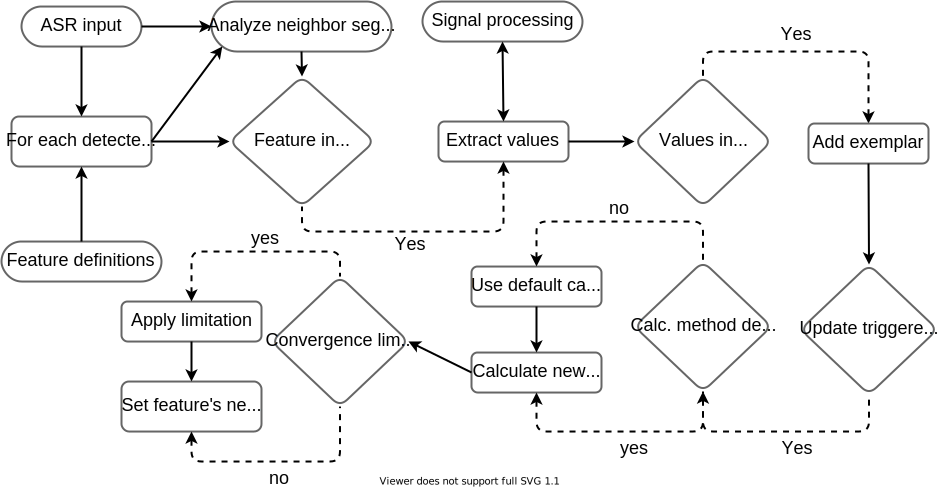
\includegraphics[width=\linewidth]{pipeline}
	\caption[Phonetic convergence algorithm pipeline]
		{Overview of the vocal accommodation pipeline.
		Rectangle nodes represent steps where an action is performed, round rectangles are inputs (either external or from the system), and diamond-shaped nodes stand for decision points.
		Nodes without a \enquote{no} edge indicate termination of the process at that point if their condition is not met (and therefore no accommodation occurs).
		The pipeline can only be successfully completed at the \enquote{Set feature's new value} node.}
		% However, if the \enquote{Add exemplar} action was performed prior to termination, the exemplar is not removed and will be taken into consideration the next time the pipeline is triggered for the feature with which it is associated.
		% The \enquote{feature definitions} come from the configuration file and can be changed by the user.}
	\label{fig:adaptation_module_pipeline}
\end{figure}

\subsection{Detect}
\label{subsec:detect}

This step stands for the human ability to identify phonemes in speech and analyze the way they are realized.
The input to this first step in the pipeline is the raw speech signal of the speaker and its output is a sequence of realizations that may contain phonetic changes.
The \ac{asr} component of the system is responsible for detecting these realizations and their timestamps in the signal.
With this information, various methods can be used to define and measure target features to take into consideration and pass forward.
\Cref{subsubsec:detecting_segment_exemplars} shows an example of such a definition and how it is used in a \ac{sds}.

An interlocutor cannot accommodate to features that are not present in a speaker's speech.
For changes on any level to happen, some pre-defined feature that is prone to change needs to be present and detected in the input speech stream.
Moreover, for the changes to register as a variation of a feature, the realization produced by the speaker must be prominent and distinctive enough to be perceived by the listener.
In the case of computers, that means a way to measure the difference between realizations and classify their distance from one another.
This difference can be categorical or continual, depending on the feature.
In addition, not only the features which introduce meaningful difference are language- and culture-dependent, but they might also differ based on the specific situation in which the interaction takes place.
For example, a segmental feature of a language where a phoneme can be realized in two alternative ways (as the allophonic alteration explained in \cref{subsubsec:target_features_HCIConv}) will probably be ignored by a speaker of a language where only one of these vowels exist in its repository.
In this case, the two vowels will simply be mentally merged into one, without causing any difficulties with comprehension.
Suprasegmental features, like \ac{f0} contour and \ac{ar}, occur globally across the speech signal and are more often cross-lingual.
Still, for a computer to be able to detect and track changes in those features, a way to measure and compare them is required.

\subsection{Filter}
\label{subsec:filter}

This step corresponds the human internal, often unconscious, linguistic knowledge, and how it is used to decide which detected realizations are valid new instances that will be stored in memory.
Its input is instances of a defined target feature detected in the previous step and it outputs those instances that should be stored as exemplars of their respective features.
\Cref{subsubsec:filtering_exemplars} demonstrates how a filter is applied based on a phonological rule and a feature definition with a target phoneme.

A target phoneme serves as an anchor for a rule that aims to capture a phonetic feature or a more evolved phonological rule.
For example, the German phonological rule of \textipa{[@]} elision at word-final \emph{-en} (as described by \cref{eq:schwa_elision_rule}) can be captured by the phoneme sequence /C\textipa{@n}/, where C represents a consonant (although in practice only a subset of the German consonants can be placed at this position).
The anchor phoneme is \textipa{[@]}, since this is the segment that is subject to the change, namely the length -- or complete absence -- of it.
therefore, for this phenomenon, the target phoneme would be \textipa{[@]} and the measured feature would be segment length.
Another target feature described in \cref{subsubsec:target_features_HCIConv} is \textipa{[e:]} vs.\ \textipa{[E:]} realization of the mid-word grapheme \emph{ä}, which is captured by the target anchor phoneme \textipa{[E]} in a non-final position of a word.
Any defined feature goes through two filters.
First, the phonological context of the detected sequence is matched against the one defined for the target feature; and secondly, the defined accepted value range that would make it an acceptable instance of that phenomenon, like \textipa{[@]} length between \SI{0}{\milli\second} and \SI{60}{\milli\second} or appropriate F$_1$ and F$_2$ values for the \textipa{[e:]} and \textipa{[E:]} vowels in the aforementioned features.
After applying these two filters, only those instances that truthfully capture the desired phonetic phenomenon are kept.
Another purpose of this step is to provide a way to integrate phonetic expertise to be used in the process.
This helps not only to be more accurate regarding language-specific knowledge, but also to prevent \ac{asr} errors to propagate further in the pipeline.

\subsection{Store}
\label{subsec:store}

\begin{figure}[t]
	\centering
	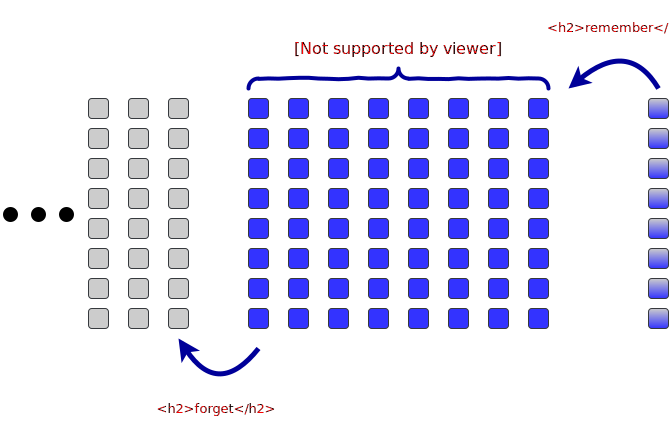
\includegraphics[width=0.8\textwidth]{pool}
	\caption[The exemplar pool]
		{Illustration of an exemplar pool.
		Each exemplar is represented by a column of squares (each representing a numeric value).
		A new exemplar is added to the feature's pool when encountered.
		Old exemplars are removed when the pool is full.
		Exemplars currently in the pool are taken into account when the realization of the feature is determined.}
	\label{fig:exemplar_pool}
\end{figure}
%
This step represents the mental phonetic memory of a speaker, here referred to as a \emph{pool} for a computer-based interlocutor.
The input to it is a feature's exemplars that passed the filtering step and its output is used for updating the feature's representation.
An illustration of an exemplar pool is shown in \cref{fig:exemplar_pool} and an implementation of it is described in \cref{subsubsec:collecting_exemplars}.

After an instance of a feature is detected and validated, it needs to be registered as an exemplar of the feature it is associated with.
This stands in parallel to the way such exemplars (and in other contexts also words, meanings, etc.) are mentally stored in the human's short- and long-term memories.
These accumulated exemplars of a feature determine how a speaker perceives it and shape its production when used in speech.
One of the complexities of modeling such internal representation is the interleaving influences of both long-term and short-term memory.
In spoken interaction, the long-term memory may define the typical productions of a user, while the short-term memory is used and changed within a single conversation.
Since this model aims to describe accommodation occurring within the scope of a single, isolated interaction (even if a long one), only the storage of exemplars encountered in this interaction is explicitly addressed in it.
However, long-term effects may be implicitly achieved by retaining values between interactions.
This step also defines how new exemplars are added, stored, and removed (cf.\ \cref{fig:exemplar_pool}).
Each feature has its own exemplar pool to which newly encountered exemplars are \enquote{memorized}, and each exemplar is a vector of the values measured for the target feature, e.g., formant values).
The pool functions in a first-in-first-out fashion, fitting the temporally linear progression of spoken interaction.
An exemplar is represented by a vector with cardinality $n$, where $n$ is the number of dimensions required for describing this feature.
Whenever an exemplar of the feature is encountered, a new exemplar is added to the pool.
The size of the pool determines the memory capacity, i.e., for how long exemplars are remembered during the interaction.
If the pool is already at full capacity, the oldest exemplar is \enquote{forgotten} when a new exemplar is added.
Ultimately, a pool of a feature can be used to determine which exemplars are still affecting the speaker's mental state of a feature.
As the order of the added exemplars is kept, it can be taken into account as well when determining each exemplar's weight, just like recent turns are more likely to influence the current utterance than turns from the beginning of the conversation.

\subsection{Update}
\label{subsec:update}

This step incorporates the process of changing the mental state of a feature based on its accumulated exemplars.
The input to it is the current state of a feature and it outputs a new value for it.

The core of the accommodation process is the change in a feature's state.
Many factors may influence this change, both internal and external.
The two main considerations in this step are one of each, namely the desired accommodation behavior and the exemplars collected from the user's speech input.
The latter is covered by the \enquote{store} step, and the former is defined using adjustable parameters that correspond to accommodation properties in humans (see \cref{tab:comp_model_parameters}).
For example, how prone is the speaker to be influenced by others' speech and how easily should the change be triggered.
The sensitivity can be constant or vary based, e.g., on how close are the speakers' productions to begin with.
A trigger might be exemplar-based, i.e., after a certain number of new exemplars were added, or time-based, i.e., every time a certain amount of turns had passed.
Another means to shape the behavior is the way the new state is computed based on the exemplars.
For example, newer exemplars or exemplars with greater distance from the current state may influence the change more.
Moreover, the general tendency to accommodate is defined in this step, e.g., converging or diverging from the user's speech, which is determined, among others, by the application and desired behavior.
A \ac{capt} system would probably not aim to align its speech to the user's, but rather diverge from it as a way to provide auditory feedback.
This computation can use simple mathematical operations (as demonstrated in \cref{subsubsec:calculating_changed_value}) or more involved data-driven statistical methods (as the one in \cref{chap:statistical_model}).

\subsection{Assign}
\label{subsec:assign}

This step mediates between the new state of a feature and its use in the system's speech output.
The input to it is the newly calculated state of a feature and it outputs a potentially altered version of this state to be used by the \ac{tts} component.

This final step of the pipeline is responsible for assigning the features' representations to the speech production of the system as an additional input to the system's \ac{tts} component.
For a \ac{tts} module that can directly control the speech output (as part of the model itself or on the outputted waveform, as discussed in \cref{subsec:speech_manipulation}),
this additional information can be used to manipulate the target features in a way that expresses the accommodative behavior of the system.
This closes the circle from a target feature produced by the user and up to the change it triggered in the system when it speaks back.
Since that means the user will now hear certain vocal characteristics that are based on their own speech, it is important to avoid a situation where the user feels imitated -- or even mocked -- by the systems.
This is an important issue that has not been considered in previous work.
To that end, this step introduces a limitation mechanism that limits the values given to the \ac{tts} component.
The values are re-evaluated if some threshold is bypassed (see \cref{eq:new_value}), to avoid such imitation from the system's side.
This mechanism also helps to prevent the system from diverging too sharply from the user.
For example, a \ac{capt} system might demotivate or frustrate the user if its speech is consistently considerably different from the user's.
From a human's perspective, this step corresponds to the natural degree to which a speakers would change their speech while talking to others.
As shown in \cref{chap:shadowing_in_sung_music_and_human_computer_interaction,chap:speech_variations_in_hhci}, this varies from feature to feature, and hence this parameter is set for each feature individually (see \cref{tab:comp_model_parameters}).
For this to work, it is important that the features are sufficiently distinguishable and clearly defined by the pipeline, so that the specified modification in the system's speech output can be properly applied in -- and only in -- the correct places, as illustrated in \cref{fig:adapted_synthesis_output}.
%
\begin{figure}[t]
	\centering
	\includegraphics[width=0.85\textwidth]{synthesis}
	\caption[Manipulated features on a synthesized waveform (illustration)]
		{Illustration of a manipulated output audio waveform.
		Each colored pin marks a phonetic features captured and processed by the pipeline.}
	\label{fig:adapted_synthesis_output}
\end{figure}

\section{Parameters}
\label{sec:parameters}

Several parameters are introduced into the pipeline described in \cref{sec:pipeline_representation} to grant degrees of freedom in shaping the accommodation behavior.
These parameters link between the theoretical, schematic model and its integration into a \ac{sds}, as demonstrated in \cref{chap:convergence_module_for_sdss}.
They are also the key to experimentation with different settings and scenarios for different applications.
The model's parameters are summarized in \cref{tab:comp_model_parameters} \citep[and cf.][]{Raveh2017Interspeech}.

\afterpage{%
	\begin{landscape}
		\begin{table}[t]
			\centering
			\vspace{1.5cm}
			\caption[Summary of computational model's parameters]
				{Computational model's parameters in their order of use.
				The colors mark parameters associates with the
				{\color{Violet}\textbf{detect}},
				{\color{BurntOrange}\textbf{filter}},
				{\color{ForestGreen}\textbf{store}},
				{\color{RoyalBlue}\textbf{update}}, and
				{\color{red}\textbf{assign}} steps.}
			\label{tab:comp_model_parameters}
			\begin{tabulary}{\linewidth}{lLL}
				\toprule
				\multicolumn{1}{c}{\textbf{Parameter}} & \multicolumn{1}{c}{\textbf{Description}} & \multicolumn{1}{c}{\textbf{Value}} \\
				
				{\color{Violet}\textbf{target phoneme}}*
				& the phoneme that triggers the feature's pipeline
				& a phoneme symbol\\\addlinespace[0.2cm]
				
				{\color{BurntOrange}\textbf{phonetic context}}*
				& the environment in which the feature instance is accepted
				& regex containing the of phoneme symbols containing target phoneme\\\addlinespace[0.2cm]
				
				{\color{BurntOrange}\textbf{allowed range}}*
				& the value range(s) in which new instances are accepted
				& two numeric values (min and max) per feature dimension\\\addlinespace[0.2cm]
				
				{\color{ForestGreen}\textbf{exemplar pool size}}
				& maximum number of exemplars in memory at a time, oldest exemplar removed when full
				& positive integer\\\addlinespace[0.2cm]
				
				{\color{RoyalBlue}\textbf{update frequency}}
				& how frequently a feature's value is recalculated, controlling the accommodation pace
				& non-negative integer; 0 for manual update\\\addlinespace[0.2cm]
				
				{\color{RoyalBlue}\textbf{calculation method}}*
				& the manner in which the pool value is calculated based on the values and order of the exemplars in pool
				& any $\mathbb{R}^{n \times m} \longrightarrow \mathbb{R}^{m}$ function; either implemented directly in code or sent to an external statistical model\\\addlinespace[0.2cm]
				
				{\color{RoyalBlue}\textbf{convergence rate}}
				& weight of the exemplar pool when updating the feature's state, controlling the impact of external input on the speaker's features states
				& real value; typically $n \in (0, 1) \subset \mathbb{R}$; 0 for ignoring the pool ; $> 1$ for over-weighting the pool value\\\addlinespace[0.2cm]
				
				{\color{red}\textbf{convergence limit}}*
				& the maximum degree of convergence allowed for the feature with respect to the input instances
				& real value; $n \in (0, 1] \subset \mathbb{R}$; 1 (\SI{100}{\percent}) for no limitation \\
				\bottomrule
			\end{tabulary}
			\flushleft{\footnotesize \emph{* denotes parameters that are defined individually for each feature}}
		\end{table}
	\end{landscape}
}

As shown in \cref{sec:convergence_to_natural_and_synthetic_stimuli}, not all participants showed the same \emph{sensitivity} toward changes in the stimuli.
Here, sensitivity refers to the degree of overall change toward external speech input.
Additionally, when one does converge, the sensitivity to changes (the \enquote{amount of differentiation}) toward a every single stimulus might differ as well.
These two aspects are jointly controlled by the \emph{convergence rate}, which represents the balance between the current and heard speech when calculating the accommodation outcome.
Generally, low convergence rate leads to a slow (and potentially unnoticeable) change, while a high rate would lead to sharper changes and that may overshoot the target, as demonstrated in \cref{tab:validation_baseline,fig:validation_sensitivity}.
To simulate the case where a speaker is not influenced by external speech input (the exemplars in the pool) at all, this rate can be set to zero.
In that case, the model will ignore the other interlocutor's speech and stick to the current speech style.
Another difference found among the participants was the total overall convergence degree toward the stimuli, i.e., where does the convergence process stop.
This is monitored by the \emph{convergence limit}, which defines the maximally allowed degree of similarity between the interlocutors.
When set to 1 (\SI{100}{\percent}), the model is allowed to change up to \SI{100}{\percent} toward the other interlocutor (complete convergence); when set to 0.8, up to \SI{80}{\percent}, and so on.
The parameter ensures that the model does not simply imitate the user's input, which is the approach often found in such system nowadays.
By limiting the change, the accommodation process is more gradual and restrained, avoiding peaks and abrupt changes.

Parameters defining the adaptation itself are not enough.
To properly model an accommodative behavior, some aspects that are not directly related to the speech output are required as well.
The accommodation process relies on the recent instances (\emph{exemplars}) of a speech sound.
How many exemplars are taken into account when the feature's state is updated depends on the interlocutor's mental memory of that sound.
This internal memory is a complex mechanism \citep{Baddeley2003working}, which is simplified here into a single parameter, namely the \emph{exemplar pool size}, which determines the number of exemplars the interlocutor currently remembers.
This exemplar history is managed on a first-in-first-out basis, so that the \emph{order} in which the exemplars were acquired is kept as well and can be used for weighting their influence.
This pool size can be tweaked to match the scenario and the expected interaction length.
The \emph{tendency to converge} toward other interlocutors also differs from speaker to speaker.
This likelihood is controlled by a parameter (a probabilistic approach for this property is discussed in \cref{chap:statistical_model}).
After an exemplar is added to a feature's pool, an update of the feature's value may be triggered.
Whether and how often this happens is determined by the \emph{update frequency}.
When set to 1, an update will occur every time an exemplar is added; if set to 2, every other exemplar, and so on.
When set to 0, however, updates will only take place when explicitly requested, e.g., after a pre-determined number of turns or a fixed amount of time.
This can be useful when all features are to be updated at the same time, regardless of how many exemplars have been accumulated for each of them.
Increasing the update interval means that each update will be affected by a higher number of new exemplars, which might result in a smoother converging process, depending on the calculation method used (see below).
Additionally, a longer update interval also means that accommodation will generally take longer, since the model's features are not being updated as frequently.
This is fitting for systems with which the user is expected to have long interactions.

Not only the frequency of updates plays a roll in the process, but also the manner in which the update is performed.
This manner is determined by the \emph{calculation method}.
Since the features in the model are represented by vectors, any function that takes a matrix as input and outputs a vector as output can be used, as demonstrated in \cref{subsubsec:calculating_changed_value}.
The method can be either statistical or deterministic, e.g., simply averaging the exemplars, but methods that can take order into account, like decaying average, might yield more realistic accommodative behaviors.
A different calculation method can be assigned to each feature, which can help to account for acoustic or psycholinguistic constraints.
This can also be influenced by the setting the system is purposed for, like experimental, exploratory, data collection, etc.

For each feature, a \emph{target phoneme} is defined, which has two purposes:
First, it tells the \ac{asr} component which phoneme is associated with this feature, so that it is forwarded for further analysis.
Secondly, it is used in the \emph{phonetic context} to filter instances of the phoneme that should not be associated with the feature.
The context is the environment in which the target phoneme should be found in the \ac{asr} output sequence for the instance to be considered\footnote{This requires an \ac{asr} engine that returns such a sequence in addition to textual output.
It is therefore crucial that the phoneme symbol set used in the model and by the \ac{asr} is the same and unambiguous, specifically when used in a regular expression.
This is the only part of the pipeline that is language-dependent (or rather symbol-dependent)
Using non-ASCII symbol sets, like IPA, may solve many of these issues, but is not recommended since \ac{asr} engines rarely use those and also due to other technical reasons.}.
For suprasegmental features -- or any other feature that is not bound to a specific phoneme or context -- the target phoneme can remain empty, so that the phonetic context would match any sequence.
The second parameter used to put constrains on the detected phones is the \emph{allowed range}, which defines the minimum and maximum acceptable values for the feature.
This parameter is important to obtain clean and sensible exemplars, as it introduces restrictions based on phonetic knowledge (e.g., reasonable \ac{f0} values for a human speaker), which at the same time also help to prevent \ac{asr} errors from meddling with the exemplars sent to the pool.
Since these values are feature-dependent, this parameter is set for each feature individually.
%\Cref{subsubsec:detecting_segment_exemplars} shows an example of a feature definition.
\chapter{Probabilistic Model}
\label{chap:statistical_model}

\lettrine{I}{ntroduction} into this chapter\dots

\pagebreak

\section{Time series representation and \aclp{gp}}
\label{sec:time_series_analysis}

\todo[inline]{introduction to GP. search over all functions. emphasize the aspects of it that we are using it for, but also a bit generally why it's good for ML. compare it to other interpolation/extrapolation methods. if makes sense, explain to what kind of data it suits.}

%\subsection{Covariance functions (kernels)}
\subsection{Kernel building and tuning}
\label{subsec:covariance_functions}

\todo[inline]{current information taken from \url{http://scikit-learn.org/stable/modules/gaussian_process.html}. in the introduction add the reference(s) mention at the end of this page.}
\todo[inline]{also, there was a very detailed thesis/paper about kernels, check if there are more good details there}

Kernels (also called \textit{covariance functions} in the context of \acp{gp}) are a key component \acp{gp}, as they define the statistical relationship between the input values.
In general, they represent describe the similarity $k(x, x')$ between each pair of input points, so that $k(\cdot, \cdot)$ determines how similar the outputs $y_*$ and $y_*'$ will be. 
More formally, a covariance function can be described as $\mathcal{K}(u, v) = \phi(u) \cdot \phi(v)$, where $\phi(\cdot)$ is a function that maps the input vectors into a transformed feature space.
Which function to use is a key question when modeling using a \ac{gp}, as it determines the behavior of the model and the quality of the predictions it will be able to make.
Naturally, some assumptions and decisions regarding the data must be made when choosing a kernel.
A kernel's parameters are optimized to achieve functions that better fit the data, the consistency of the resulted functions is measured using log maximum likelihood.

Since convergence analyses usually refer to the \textit{difference} between values in different production (as opposed to the values themselves), stationary kernels are more suitable for fitting \ac{gp} to them, as they are shaped by the distances between each pair of data point rather than merely their absolute values.
%That is, they fulfill $k(x_1, x_2) = k(x_1 - x_2)$.
%This list only covers a small subset of common covariance functions.
%Further kernels include the exp-sine squared, dot-product, linear, and more.
%\putref{put 2 references about kernels, or only 1 is the first is used above}
Kernels can also be chained using multiplication or addition to combine characteristics of multiple kernels.
Multiplication-based kernels are maximized when all of its kernel factors yield high values, whereas
Addition-based kernels, are maximized when any of their addend kernels yield a high value.
%For example, multiplying a linear kernel by a periodic one will result in functions that are \textit{both} periodic \textit{and} with increasing amplitude as they move away from the origin.
For the modeling presented here, an additive kernel is used with constant, RBF, and noise terms (see \crefrange{eq:constant_kernel}{eq:RBF_kernel}).
The RBF term determines the general shape of the curve (see example in \cref{fig:RBF_prior_posterior}), the constant term enables shifting of the curve if necessary, and the noise term adds degrees of freedom in case the curve cannot completely fit the input signal.

The definitions of the used kernels are as follows:

\begin{description}
	\item[Constant kernel -- ]
	This is a simple kernel that assigns the same value for all input pairs.
	Since by itself it does not offer a lot of characteristic to the covariance function, it is usually used as part of a product kernel, where which it scales the magnitude of the other factors, or as part of a sum kernel, in which it modifies the mean of the Gaussian process.
	It has a single parameter, the constant value, and it is defined as 
	%
	\begin{equation}
		\label{eq:constant_kernel}
		k_{constant}(C, x, x') = C\forall x_1, x_2,
	\end{equation}
	\eqname{Constant kernel}
	%
	where $C$ is the constant value parameter.
	
	\item[Noise kernel -- ]
	is a kernel used for capturing unexplained variation in the data, i.e., noise.
	It is typically based on the constant kernel as part of a sum kernel, in which it explains the noise component of a signal.
	In this context, the constant parameter is tuned to estimate the noise level.
	This is determined by
	%
	\begin{equation}
		\label{eq:noise_kernel}
		k_{noise}(\{noise\_level\}, x, x') =
		\begin{cases}
		C_{noise\_level}, & if\quad x_1 = x_2\\
		0, & otherwise,\\
		\end{cases}
	\end{equation}
	\eqname{Noise kernel}
	%
	where $noise\_level$ equals the variance of the noise found in the input signal.
	
	\item[Radial-basis function (RBF) kernel --]
	also known as \emph{squared exponential kernel}, the RBF kernel is a stationary kernel with one parameter, \emph{lengthscale} $l > 0$.
%	 which can either be a scalar (isotropic variant of the kernel) or a vector with the same number of dimensions as the inputs x (anisotropic variant of the kernel).
	This kernel typically results in generally smoothed functions, with the lengthscale being associated with the long-term smoothness and degree of variability on the time dimension.
	The RBF kernel is defined as
	%
	\begin{equation}
		\label{eq:RBF_kernel}
		k_{RBF}(\{\ell\}, x, x') = \sigma^2 exp\left(\frac{\lVert x_1 - x_2 \lVert ^2_d}{2\ell^2}\right),
	\end{equation}
	\eqname{Radial basis function (squared exponential) kernel}
	%
	where $\lVert x_1 - x_2 \lVert$ is the Euclidean distance between two $d$-dimensional input points and $\sigma^2$ is a scalar factor that determines the average distance of your function away from its mean.
	\cref{fig:RBF_prior_posterior} shows prior and posterior examples of the RBF kernel.
	
%	\item[Rational quadratic kernel]
%	This kernel can be seen as a scale mixture (infinite sum) of RBF kernels with different length scales.
%	Therefore, \acp{gp} priors with this kernel expect to see functions which vary smoothly across many length scales.
%	It has two parameters: length scale $l > 0$ and scale mixture $\alpha > 0$.
%	The parameter $\alpha$ determines the relative weighting of large-scale and small-scale variations.
%	When $\alpha$ $\lim$ $\inf$, the RQ kernel is identical to the SE kernel, as described by
%	
%	\begin{equation}
%		\label{eq:RQ_kernel}
%		k_{RQ}(\{\sigma, \alpha, \ell\}, x, x') = \sigma^2 \left( 1 + \frac{\lVert x_1 - x_2 \lVert ^2}{2\alpha \ell^2} \right)^{-\alpha}.
%	\end{equation}
%	\eqname{Rational quadratic kernel}
\end{description}

\subsection{Data interpolation using kriging}
\label{subsec:interploating_data_using_kriging}
	
\begin{figure}[t]
	\centering
	\subfigure[RBF kernel prior ($length scale = 1$)]
		{\includegraphics[width=0.45\textwidth]{RBF_prior}
	\label{fig:RBF_prior}}
	\hfill % no empty line here to avoid staring a new paragraph (figures will be vertically aligned)
	\subfigure
	[RBF kernel posterior ($length scale = 0.279$)]
	{\includegraphics[width=0.45\textwidth]{RBF_posterior}
	\label{fig:RBF_posterior}}
	\caption[Prior and posterior of RBF kernel]
		{\hspace{-0.18cm}\footnotemark\ 
		Prior and posterior distributions of an RBF kernel with mean zero, resulted in a Gaussian process $\mathcal{GP}\left( 0 (\vec{x}), \Sigma(\vec{x}) \right)$.
		Each color line stands for a drawing (prediction) from the prior and posterior distributions, and the thicker black line shows the overall mean of the distributions.
		The red circles are the known data points on which the kernel was optimized to fit, and the gray areas mark the \SI{95}{\percent} confident intervals above and below the overall mean.
		The length scale parameter (in parentheses) determines the length of the \enquote{wiggles} of the functions}
	\label{fig:RBF_prior_posterior}
\end{figure}
\footnotetext{adapted from \url{https://scikit-learn.org/stable/_images/sphx_glr_plot_gpr_prior_posterior_001.png}}

As also motivated in \cref{subsec:limitations_of_did,subsec:temporal_analysis}, artificially splitting interactions into a fixed, pre-determined number of parts to measure accommodation results in a partial view on the process.
To avoid that, some interpolation method is required, with the goal of yielding a more general behavior based on the observed productions.
This allows analysis on continuous series of values instead of point-by-point comparison, where the temporal gaps between data points might be greatly unbalanced.
One way of achieving that, using \ac{loess}, is shown in \cref{fig:hds_dds_time_pitch}.
A more evolve approach is presented here, where a speaker's vocal behavior is described as a distribution of functions that match the accumulated \textit{evidence} from the speaker's productions.

\citet{Galvez2020unifiying}\\ % compare to the rather simplistic (and naive) approach taken here (based on TAMA)
\citet{Kousidis2008towards}\\ % original TAMA paper. read again, but seems like it's glorified moving average. say that my appraoch actually learns the curve of the speaker and doesn't just interpolate, which allows continuous predictions and more evolve description.
\citet{Kousidis2009monitoring}\\ % another TAMA paper, with an a bit more concrete example

Kriging (or \textit{\acl{gp} regression}) is an interpolation method that gives an optimally fitted and unbiased prediction of intermediate values.
\todo{references for a few fields where it is used?}
Since this method fits a function distribution over the data, it not only yields mathematically more likely values, but also provides a curve that describes the characteristics of the interpolated curved, as opposed to more naive methods like linear interpolation or smoothing spline.
Another advantage of this method is that it yields a \textit{distribution over functions} rather than specific values.
Therefore, an infinite number of suitable values can be drawn from one fitted kernel and their likelihood can be evaluated.
Such interpolation is illustrated in \cref{fig:RBF_posterior}, where each line represents a mean regression prediction drawn from the posterior distribution based on the given data points.

This method was applied on the dataset presented in \cref{sec:vacc}.
For simplicity, only the interactions in solo condition were used.
The functions prediction for a each speaker can be described by
%
\begin{equation}
	\label{eq:gp_function_prediction}
	f_*(\vec{x}) = \mathcal{GP}(\mu_{speaker}, \Sigma_*),
\end{equation}
\eqname{Function predicted using a fitted Gaussian process}
%
where $\mu_{conv}$ is the mean feature value of a single speaker and $\Sigma_*$ is the fitted additive covariance function described in \cref{subsec:covariance_functions}.
It is important to note that the mean is not zeroed (as usually done in \ac{gp} regression) to maintain the original input values for the subsequent steps.
The kernel was initialized with the priors $C = 1$, $lengthscale = 1$, and no assumptions regarding noise level.
The search boundaries for the RBF and noise components were $1 < lengthscale < 100$ and $\num{1e-4} < \xi < 10$, respectively, with a maximum of six optimization iterations. % the initial one plus five allowed restarts (n_restarts_optimizer parameter in code)
\todo[inline]{make sure these numbers are up to date}
\todo[inline]{write about how datapoints where selected from each turn to represent points of change}
With the fitted kernel, a continuous prediction can be made for each speaker over the entire conversation time span.
\Cref{fig:gp_vacc} shows an example of \ac{gp} predictions for one of the conversations. % 20171121A_Calendar_01 was used
%
\begin{figure}[t]
	\centering
	\includegraphics[width=\textwidth]{GP_VACC_with_draws}
	\caption[Gaussian process regression on conversation with Alexa]
		{Gaussian process regression for an interaction of a subject with Alexa.
		 The thick blue and red lines show the predictions' mean.
		 The additional lines around the means are randomly drawn functions from the fitted kernel representing potential variational output.
		 The colored areas around the means lines show the \SI{95}{\percent} confident interval for the distributions of the same color.
		 The straight horizontal lines indicate the overall mean of each speaker's productions.
		 The posterior parameters and the log marginal likelihoods of the fitted distributions are stated at the top.}
	\label{fig:gp_vacc}
\end{figure}

\section{Marking degrees of change}
\label{sec:measuring_changes}

Once a regression line is drawn for each speaker from their respective distributions, the differences between the speakers' productions can be measured.
Furthermore, due to the higher temporal resolution, more fine-grained degrees of change over time can be calculated as well.
The differences are calculated by the subtracting the trapped areas between the two regression lines (see \cref{fig:gp_vacc})
%
\begin{equation}
	f_{diff} \equiv\Delta\vec{x}_* =
	\int_{\vec{x}_i}^{\vec{x}_{j}}\mu_{f_*subject} -
	\int_{\vec{x}_i}^{\vec{x}_{j}}\mu_{f_*alexa}
\end{equation}
% - 
and the directional derivatives of the resulted delta line to measure the degree of change
%
\begin{equation}
	\nabla\Delta\vec{x}_*' = \frac{d}{dx}f_{diff}
\end{equation}
%
along the difference line.
\Cref{fig:diff_and_derivatives} demonstrates this on the same conversation from \cref{fig:gp_vacc} using the mean predictions of each speaker.
%
\begin{figure}[t]
	\centering
	\includegraphics[width=\textwidth]{diff_and_derivatives}
	\caption[Continuous integral differences and derivatives in a \acl{hci}]
		{Continuous integral differences (red line) and their corresponding derivatives (blue line) of speakers' productions in a conversation.}
	\label{fig:diff_and_derivatives}
\end{figure}
%
For building a generative model as described in \crefrange{sec:accommodation_as_a_lm}{clustering_and_incremental_generation}, the changes must be marked with pre-defined labels.
To that end, the derivative values were translated into a continuum of change ranging from \textit{divergence} to \textit{convergence}.
Based on this continuum, a discrete scale can be defined.
The more categories this discrete scale offers, the more specific the behavior descriptions can be.
\Cref{fig:cont_disc_scales} shows this process for a discrete scale of three categories: divergence, no (major) change, and convergence.
%
\begin{figure}[t]
	\centering
	\subfigure[Continuous scale]
		{\includegraphics[width=0.47\textwidth]{cont_scale}
	\label{fig:continuous_scale}}
	\hfill
%	\vspace{-1cm}\hfill\hspace{-1cm}{\hbox{\LARGE $\Longrightarrow$}}\hfill
	\subfigure[Discrete scale]
		{\includegraphics[width=0.47\textwidth]{discrete_scale}
	\label{fig:discrete_scale}}
	\caption[Continuous and discrete scales for labeling degrees of change]
		{Continuous and discrete color-coded scales for labeling degrees of change in a conversation.}
	\label{fig:cont_disc_scales}
\end{figure}
\todo[inline]{more details regarding how the discrete categories are defined}


\section{Accommodation as a language model}
\label{sec:accommodation_as_a_lm}

\subsection{Dimensionality reduction and symbolic representation}
\label{subsec:dim_reduction_and_symbolic_rep}

\subsection{Sequence extraction and probabilities}
\label{subsec:word_extraction_and_seq_prob}

\section{Clustering and incremental variational generation}
\label{clustering_and_incremental_generation}

\todo[inline]{if this really works decently, refer to this section when describing variational vocal behavior as one of the levels for accommodative SDS}

\part{Application}
\label{part:application}

\chapter[Convergence Module for Spoken Dialogue Systems]{Convergence Module for\\Spoken Dialogue Systems}
\label{chap:convergence_module_for_sdss}

\lettrine{T}{his} chapter introduces a computational model for measuring and applying phonetic convergence as well as a plug-and-use \acs{sds} module that integrates this model.

\pagebreak

\section{Modularization}
\label{sec:modularization}

%\begin{figure}[t]
%	\centering
%	\includegraphics[width=\linewidth]{adaptation_module_pipeline}
%	\caption[Adaptataion pipeline for convergence module] {
%		Overview of the phonetic convergence pipeline used in the computational model. Rectangles
%		represent steps where an action is performed, round rectangles are inputs (either for external resources
%		or from the system), and diamonds stand for decision points. When a decision node does not have a “no”
%		outcome it means that the process is terminated (and therefore no convergence occurs) if the condition
%		is not met. The pipeline can only be successfully completed at the “Set feature’s new value” node.
%		However, if the “Add exemplar” action was performed prior to termination, the exemplar is not removed
%		and will be taken into consideration the next time the pipeline is triggered for the feature with which it is
%		associated. The “Feature definitions” come from the configuration file and can be changed by the user.
%	}
%	\label{fig:adaptation_module_pipeline}
%\end{figure}
\todo{here make an algorithm version of the pipeline (the figure comes later)}

\subsection{Computational model}
\label{subsec:computational_model}



\todo[inline]{some intro}

\subsubsection{Detecting segment exemplars}
\label{subsubsec:detecting segment exemplars}

The first step in the model is detecting segment in the user's utterance that can be ascribed to phonetic features the model aims to converge to.
This is done using CMU Sphinx\footnote{\url{https://cmusphinx.github.io/}} with some added functionality for omitting phoneme-level segments.
These features are defined, among other things, in a configuration file that is loaded by the model.
Each feature is represented by a YAML\footnote{YAML Ain't Markup Language \url{http://yaml.org/}} dictionary entry, which in turn contains a dictionary itself, where each key-value pair refer to a property of that feature.
For example, the entry

\begin{Verbatim}[tabsize=4, commandchars=\\\{\}]
- \textbf{`@\_length'}:
\textbf{phoneme}: AX
\textbf{context}: '.+ AX N'
\textbf{initial}: 0
\textbf{minimum}: 0
\textbf{maximum}: 80
\textbf{measure}: duration
\textbf{calculation}: decaying average
\textbf{sensitivity}: 0.5
\end{Verbatim}
\noindent
represents the feature \textit{@\_length} (length of a segment containing the phoneme schwa (\textipa{@})), which is indicated by \textit{AX} (value of the \textbf{phoneme} key) in the German CMU phoneme set.\todo{make sure this is really the phoneme set the system uses}
The value of the key \textbf{measure} is duration, which means that this feature is measure by the segment's length, as its name suggests.
Further more, the initial value in the model for this feature is 0 (\si{\milli\second}).
More properties will be explained in the subsections below.
This step is performed for each feature separately against each recognized phoneme (see \cref{alg:comp_model}).
Phonemes not ascribed to any defined feature are ignore.

\subsubsection{Filtering exemplars}
\label{subsubsec:filtering_exemplars}

Seeing that the target features are detected merely based on a phoneme, in which they might occur, additional filtering is required to retain only those instances where is does.
For example, the target feature \textit{@\_length} introduced in \cref{subsubsec:detecting segment exemplars} aims to capture the German phonological process of elision or epenthesis of \textipa{@} in word-final \textit{-en}\todo{put angle brackets around this}, as described by the rule (simplified version adapted from \citet[pp.\,142--143]{Benware1986phonetics}):

\begin{equation}
	\label{eq:schwa_elision_rule}
	\text{\textipa{@}}\longrightarrow \varnothing \diagup
	\left[\text{-son}\right] \ \_\_ \ \{\text{\#}, \left[\text{+const}\right]\}.
\end{equation}
\eqname{Phonological rule: schwa elision}

This filtering step comes to add any linguistic considerations related to the phonetic feature beside the phoneme itself.
Such considerations can phonemic context (defined as a phoneme regular expression in the \textbf{context} property) or range of acceptable values (defined by the \textbf{minimum} and \textbf{maximum} properties).
In the case of \textit{@\_length}, the phonemic context corresponds to a (simplified) context of the phonological rule described in \cref{eq:schwa_elision_rule}, and the value range defines the minimum and maximum length of the segment.
The range's goal is to filter out segments with unrealistic values (extremely long segment, unreliable formant values, etc.).
Any linguistic knowledge about the feature should be reflected in this step.
This important to make sure that all exemplars taken into account when calculating a new value for the feature (see \cref{subsubsec:calculating_changed_value} are sensible, to prevent unstable behavior of the model due to lack of linguistic knowledge or \ac{asr} and signal processing errors.

\subsubsection{Collecting exemplars}
\label{subsubsec:collecting_exemplars}

\todo{since in the ``theoretical'' part in Part 2 we say that this somehow represents both long and short term memories, explain that here we only deal with short memory explicitly, and long term memory is implicitly expressed by the starting value of the feature, i.e., the general (neutral) production of a speaker when no external influence is present,}

The remaining exemplars after filtering are stored and can be represented by a matrix $\mathcal{F}$, which contains the values of these exemplars.
As mentioned above, the exemplars are detected based on definition of each feature separately, and therefore each matrix $\mathcal{F}$ contains exemplars of a single feature.
Each exemplar is a row and each column is a dimension of this feature (e.g., a formant in a \textit{vowel quality} feature):

\begin{equation}
\label{eq:feature_matrix}
\mathcal{F} =
\begin{bmatrix} 
v_{11} & v_{12} & \dots  & v_{1m}\\
v_{21} & v_{22} & \dots  & v_{2m} \\
\vdots & \vdots & \ddots & \vdots \\
v_{n1} & v_{n2} & \dots  & v_{nm} 
\end{bmatrix}
\end{equation}
\eqname{A matrix of a phonetic feature}

\noindent
For example, the value $v_{21}$ is the first dimension of the second exemplar of the feature.
The model also defines a \textit{pool size}, which determines how many exemplars are kept for each feature.
This parameter aims to represent short-term mental memory of a feature's pronunciation.
That is, people are more likely to converge to utterances they heard recently than to something they heard before.\todo{can we say such a ``factual'' sentence without any reference/explanation?}
When a new exemplar is intercepted (after filtering), it is added to the pool (memory).
When a feature's pool is full (i.e., it reached its maximal size), the oldest exemplar is removed (forgotten) to make space for the newest one.
the exemplars in the pool are later used for calculating the system's change (\cref{subsubsec:calculating_changed_value}).
To calculate the change for each dimension (or sub-value) of a feature (like each formant of a vowel), the feature matrix is first transposed:

\begin{equation}
\label{eq:transposed_feature_matrix}
\textbf{$\mathcal{F}$}^\top =
\begin{bmatrix} 
v_{11} & v_{21} & \dots  & v_{n1}\\
v_{12} & v_{22} & \dots  & v_{n2} \\
\vdots & \vdots & \ddots & \vdots \\
v_{1m} & v_{2m} & \dots  & v_{nm} 
\end{bmatrix}
\end{equation}
\noindent
In this matrix, each row refers to a single dimension of the feature.
For example, the second row contains the value of the second dimension of each exemplar.

\subsubsection{Calculating a new value}
\label{subsubsec:calculating_changed_value}

The new value of a feature is calculated based on its exemplar pool (\cref{eq:transposed_feature_matrix}).
The relation between these values and the new value the system will use for this feature is a key aspect of the whole process.
A \textit{calculation method} is needed to define this relation ship.
Different calculation methods can represent different types of relations and approaches.
We define a function $g$ that maps a vector to a scalar (one feature dimension) and a function $\mathcal{G}$ which maps a matrix to a vector (the entire feature) by applying $g$ to all the row vectors in $\mathcal{F}$, both based on a user-defined calculation method:

\begin{equation}
\label{eq:matrix2vec}
g: \mathbb{Q}^{m} \longrightarrow \mathbb{Q}, \qquad \mathcal{G}: \mathbb{Q}^{n \times m} \longrightarrow \mathbb{Q}^{m} 
\end{equation}

\textit{Decaying average} was used as a baseline method.
This measure is similar to normal average, only that in this variation each value contributes exponentially less to the overall average, so that the last (newest) value contributes the most.
Adding such property to the measure gives more weight to new exemplars that were received chronologically closer to present time, and less weight to older exemplars that stayed longer in memory (and had more weight when they were new).
Using this measure comes to support the analogy of the exemplar pool to short-term memory, which remembers recent event better than oder ones.
Decaying average is a recursive measure described by
\begin{equation}
\label{eq:decaying_average}
\mu_n = \frac{1}{n}\sum_{i = 2}^{n}(\eta v_i + (1 - \eta )\mu_{i-1}),
\end{equation}
\eqname{Decaying average}
%
with $n$ being the number of elements in a row of the transposed feature matrix (\cref{eq:transposed_feature_matrix}), $\eta$ the decay rate, $\mu_{i-1}$ the decaying average of the previous element, and $v_i$ the value of the $i$-th element.
However, every function that can map vectors to scalars can be used here to experiment with different methods.

Before setting the updated value as the feature's value (see \cref{subsubsec:setting_the_new_value}), the balance between the feature's current value and its calculated pool value needs to be set.
This is defined by the \textbf{sensitivity} property (or \textit{convergence rate}).
The purpose of this parameter is to model the speaker's sensitivity to changes (hence the properties name), and it is used as follows:

\begin{equation}
\Upsilon \equiv \mathcal{C}_u = \rho \upsilon + \left(1 - \rho \right) \mathcal{C}_{u-1} 
\label{eq:convergence_rate}
\end{equation}
\noindent
where $\Upsilon$ is the new feature value (i.e., the value after update $u$), $\upsilon$ is the calculated pool after applying $\mathcal{G}$, $\mathcal{C}_{u-1}$ is the current value of the feature (after the previous update), and $\rho$ is the convergence rate.
A $\rho$ value of 0 means that no convergence occurs (the current value is retained), a value of 1 will result in complete convergence (the current value is ignored), and $\rho=0.5$ will result in an average between the two.
While the convergence rate is typically a value between 0 and 1, smaller and greater values could be meaningful in some applications to achieve divergence or over-convergence, respectively.

Having found in previous work that people's convergence in both \ac{hhi} and \ac{hci} varies considerably \citep{Gessinger2017Interspeech}, this parameter needs to be tuned with respect to the other parameters to obtain convergence steps that are comparable to natural speech convergence.
It can be use to achieve certain behaviors during the interaction.
For instance, in a tutoring system for pronunciation training, the desired behavior might be for the system to diverge from users' input when it detects that their pronunciation is wrong.
By reflecting the users' utterance with diverged pronunciation (instead of explicitly pointing out their mistake), the user receives auditory feedback in a more \enquote{conversational} learning process.

%\begin{equation}
%	\lambda\mathcal{M} = \lambda
%	\begin{pmatrix} 
%		v_{11} & v_{12} & \dots  & v_{n}\\
%		v_{21} & v_{22} & \dots  & v_{2n} \\
%		\vdots & \vdots & \ddots & \vdots \\
%		v_{e1} & v_{e2} & \dots  & v_{en} 
%	\end{pmatrix}
%\end{equation}
%
%\begin{equation}
%	\mathcal{M}_i' = g(\mathcal{M}^{\intercal}_{i \leq m})
%	\label{eq:value_calculation}
%\end{equation}
%\noindent
%where $\mathcal{M}^{\intercal} \in \mathbb{Q}^{m \times n}$ is the transposed exemplar matrix (which comprises vectors of dimension values instead of vectors of exemplar values), $g$ is the chosen calculation method to apply to each vector, $\mathcal{M}' \in \mathbb{Q}^{m \times n}$ is the matrix with the pool values for each dimension of the feature, $i$ is the vector index, and $m$ is the number of rows in $\mathcal{M}^{\intercal}$.

%$\lVert P \rVert $ refers to the Euclidean Norm (or vector's magnitude).

\subsubsection{Setting the new value}
\label{subsubsec:setting_the_new_value}
\todo[inline]{mention also that we limit the final value to prevent imitation}

The final step is to set the newly calculated value (\cref{subsubsec:calculating_changed_value} as the new value for the feature in the model.
After this step ,this new value will be used whenever this feature is used by a system using this model (more details in \cref{subsec:computational_model}).
Although this step is fairly straight forward, there is still an important issue to take into consideration here, namely \textit{user imitation}.
After some turns (or with a certain combination of parameter values), it might happen that the model calculated a value very close to the user's input.
To avoid imitation, the new value is limited in how close it is allowed to get to the exemplars.
This is done by the global property \textbf{ConvergenceThreshold}, which defines the maximally allowed proximity (in percentage) the new value is allowed to have:
Setting this property to 0.8 (\SI{80}{\percent} means that the new value is not allowed to be changed more than (\SI{80}{\percent} of the difference between the current value and the pool's value (and be set to (\SI{80}{\percent} in case it exceeded this threshold).
Of course, the limitation can also be set to 1 to allow the new value be as similar as \SI{100}{\percent} to the pool's value -- i.e., not limiting it.
The maximal value allowed by the limitation is defined by

\begin{equation}
\label{eq:conv_limit}
\Lambda = \delta \upsilon \left(1 - \lambda \right),
\end{equation}
\noindent
where $\Lambda$ is the maximum convergence value allowed, $\delta$ is set to 1 if the converging values are increasing or $-1$ in case they are decreasing (see \cref{eq:direction}), and $\lambda$ is the convergence limit parameter ($\lambda=0.8$ in the example above).
\noindent
Note that the actual value of this limit depends on the direction in which the convergence occurs, which is defined by

\begin{equation}
\label{eq:direction}
\delta = 		
\begin{cases}
\ \ \ 1 & \text{if } \upsilon \geq \mathcal{C}_t\\
-1 & \text{otherwise}
\end{cases}.
\end{equation}
\eqname{Determining accommodation direction}
\noindent
That is, if the converging values are increasing, the limit's value will be smaller than the pool value;
and if the values are decreasing toward the pool value, the limit's value will be greater than the pool value.
Ultimately, the final updated value for the feature is determined as follows:

\begin{equation}
\label{eq:new_value}
\Upsilon = 		
\begin{cases}
% newValue - (newValue - (newValue * convergenceThreshold)) * direction
\upsilon - \Lambda & \text{if }\upsilon - \Upsilon \leq \delta\Lambda\\
\Upsilon \text{ (unchanged)} & \text{otherwise}
\end{cases}.
\end{equation}
\eqname{Setting accommodation limit}
\noindent
It is important to mention that this limitation not only comes to prevent situations where the model mimics and user's behavior (which might lead to intimidation), but is also loyal to behaviors observed in the experiment, where participants only converged up to a certain limit, hence the name of this property.

The entire computational model is described in \cref{alg:comp_model}.
Further details about the model and all the steps can be found in \citet{Raveh2017Interspeech}.

\begin{algorithm}[t]
	\caption{Phonetic responsiveness}
	\label{alg:comp_model}
	\eqname{Phonetic responsiveness algorithm}
	\algorithmcaption{Note that \emph{ASRInput} (\cref{line:asrinput}) must not only contain the $n$-best hypotheses, but also their phoneme lists (in chronological order).
	For improving performance, using a single hypothesis is recommended for a small language model and/or when very short sentences are expected.
	Since only the target phonemes are treated (and suprasegmental features where the specific phonemes do not matter), it might not be crucial to get a completely correct \ac{asr} hypothesis if not required for continuing the interaction.
	For example, a \ac{capt} system might rely solely on the realization of specific phonemes, regardless of what the user said or should have said.}
	\DontPrintSemicolon
	\SetKwInOut{Input}{Inputs}
	\SetKwInOut{Output}{Output}
	
	\Input{\underline{$ASRInput$} -- recognized user speech\newline
		   \underline{$targetPhonemes$} -- convergence features\newline}
	\Output{list of feature vectors with converged values\newline}
	
	\ForEach {(phoneme $\in$ ASRInput) $\in$ targetPhonemes}{ \label{line:asrinput}
		$feature \gets$ $phoneme$.associatedFeature\;
		$context \gets feature$.phoneticContext\;
		\uIf {\textbf{not} matches(phoneme, context)}{ \tcp*{filter based on context}
			break\;}
		\uIf {inRange($phoneme$, $allowedRange$)}{ \tcp*{filter based on value range}
			\uIf {poolSize=maxPoolSize}{
				deleteOldestExemplar()\;}
			feature.addExemplar($phoneme$)\;}
		\uElse{
			break\;}
		\uIf {toUpdate $=0$}{
			$method \gets feature$.calculationMethod\;
			$poolValue \gets method$.calculate(pool)\;
			$newValue \gets rate\cdot poolValue + (1-rate)\cdot feature.$value\;
			$threshold \gets convergenceLimit \cdot poolValue$\;
			\uIf {$newValue > threshold$}{ \tcp*{limit convergence}
				$newValue \gets threshold$\;}
			$feature$.value $\gets newValue$\;
			{\em toUpdate $\gets$ updatefrequency}\;}
		\uElse{
			{\em toUpdate $\gets$ toUpdate - 1}\;}}
\end{algorithm}
\todo[inline]{make algorithm more readable, change, variable/method names, etc.}

\section{Integration}
\label{sec:integration}

\begin{figure}[t]
	\centering
	\includegraphics[width=\linewidth]{sds_architecture_ext}
	\caption[Proposed extended architecture of a spoken dialogue system] {
		Suggested architecture for a spoken dialogue system with the phonetic convergence module (conf.\ \cref{fig:sds_architecture}).
		The module connects the \ac{asr} and the \ac{tts} modules, and performs additional speech processing used phonetic for adaptation, like feature detection and extraction.
	}
	\label{fig:adaptation_module_architecture}
\end{figure}

\chapter{Web-Based Responsive Spoken Dialogue System}
\label{chap:web-based_responsive_spoken_dialogue_system}

\lettrine{I}{ntroduction} to this chapter\ldots
% complete, web-based \ac{sds} with focus on vocal adaptation.

\pagebreak

\section{Overview and key aspects}
\label{sec:overview_and_key_aspects}

Simulating and triggering accommodation effects occurring in \ac{hhi} like those found in \cref{chap:conv_analysis} in \acp{sds} takes them one step further toward human-like communication.
The system presented in this chapter encapsulates the knowledge acquired from the experiments in \cref{part:experiments}, the behavior designs developed in \cref{part:modeling}, and the module introduced in \cref{chap:convergence_module_for_sdss} which enables the vocal changes.
It contains mechanisms to track the states and changes of segment-level and suprasegmental-level phonetic features during a dialogue.
All the analyses are automated and run in real-time, which not only saves a lot of time and manual work typically needed in convergence studies, but also makes the system more suitable for integration into other applications.
It holds the following key principles:
%
\begin{description}
	\item[Focus on adaptation] --
	the main goal of the system is to offer a tool for investigating vocal accommodation in \ac{hci} for both online experiments and offline analyses.
	Putting vocal accommodation under the spotlight is the core novel contribution of the system, as very few systems offer such capabilities at all, and with control over the accommodative behavior in particular.
	
	\item[Customizability] --
	the system includes several components that can be modified, either for changing the accommodation behavior itself (features, parameters, etc.) or changing the setting (e.g., for different experiments).
	This allows experimenting with different scenarios and configurations and easily compare them in a controlled, reproducible environment.
	
	\item[Online scalability] --
	the system can run in a web browser without any installations or additional files\footnote{some features need to be enabled in the browser, like JavaScript and microphone access.
	However, any modern browser should not have any problem supporting all the necessary requirements.
	To increase performance, all speech analyses and processing are done on the server side.}.
	Since the system itself runs on a single server, it is also possible to operate multiple instances, each with its own configurations and parameters.
	This makes it easy to distribute, e.g., for remotely conducting an experiment where each participant may receive a different configuration.
\end{description}
%
Ultimately, this customizable system could help to deepen the experimental possibilities and automating some aspects of the processes convergence-related experiments typically comprises.
The system's architecture, and \ac{gui}, and functionality are described in \cref{sec:architecture,sec:online_and_offline_paths}.
The experiment presented in \cref{chap:shadowing_experiment_with_natural_and_synthetic_voices} is replicated in \cref{sec:showcase} to demonstrate the system's utilization.

\section{Architecture}
\label{sec:architecture}

As the system aims to offer a customizable playground for experimenting and studying phonetic adaptation in \ac{hci}, a key aspect of its architecture is the separation between client-side, server-side, and external resources (see \cref{fig:web-based_architecture}).
This separation makes it possible to run multiple clients on different machines at the same time with a single server collecting the data from all of them at the same time.
The server, ideally running on a dedicated machine, is operated by an a person responsible of designing and configuring the interactions, e.g., an experimenter.
It collects information and audio recordings from all interactions with the system (which can be deleted afterwards for privacy purposes).
This separation of the server grants the experimenter a lot of freedom and flexibility, since resources like feature configurations and dialogue domain can be modified independently of specific machines interacting with the system.
Additionally, multiple configurations can be prepared in advance (e.g., for different participant groups), regardless of the device the experiment will be performed on and before summoning the participants.
Configurations can even be changed mid-interaction.
These configurations are transparent to the users, and no effort is required from them (aside from start a new interaction in the case of some specific configurations).
This flexibility makes it easier and quicker to create new scenarios of interaction and to experiment with different features and parameters.

In addition to the technical advantages, letting users interact with the system on a separate machine broadens the usage possibilities.
For example, an experiment can be carried out remotely, without the need to invite participants to the recording studio one by one.
Furthermore, as the connection to the server is done via a web browser, participants can connect use the system with their own computers wherever and whenever it suits them, without any additional installation or technical configurations.
All of these makes it possible to collect data from many users rapidly and easily.
%
\begin{figure}[t]
	\centering
	\includegraphics[width=\linewidth]{web-based_architecture_no-ajax}
	\caption[Architecture of a web-based responsive spoken dialogue system]
		{The architecture of the web-based responsive spoken dialogue system.
		The background colors distinguish between client components, server components, and customizable external resources.
		The dashed line indicates that the feature predictions may or may not be passed from the model to the system depending on the feature definition and update parameter.}
	\label{fig:web-based_architecture}
\end{figure}
%
As shown in \cref{fig:web-based_architecture}, the main components of the system are the \ac{sds} itself (including the accommodation module; \cref{subsec:dialogue_system}), the \ac{gui} (\cref{subsec:graphical_user_interface}), and the external resources and configuration (\cref{subsec:models_and_cusomizations}).

\subsection{Dialogue system}
\label{subsec:dialogue_system}

The core of the system is the dialogue system component (see \cref{fig:web-based_architecture}), which controls the flow of the interaction, processes user's inputs, and generates the system's responses.
It uses the extended architecture presented in \cref{subsec:extended_sds}, which consists of typical \ac{sds} components such as \ac{nlu} and a \ac{dm}, but also contains the \ac{asp}  module that adds accommodation support \citep{Raveh2017SemDial}.
The implementation of this module in the system is as described in \cref{fig:adaptation_module_architecture}.
While the \ac{nlu} component uses merely the transcription provided by the \ac{asr}, the \ac{asp} module analyzes the speech signal itself.
Concretely, it tracks occurrences of the defined features and passes their measured values to the convergence model, as explained in \cref{subsubsec:tracked_features}, which, in turn, forwards the tracked feature parameters to the \ac{tts} synthesis component.
The \ac{tts} engine then takes the text generated by the \ac{nlg} component, and, if phonetic-level manipulation is supported, synthesizes the utterance using the values specified by the convergence model.
The connection between the dialogue system's modules is managed by the \emph{OpenDial} framework \citep{Lison2016opendial, Lison2015developing}.
The \ac{asr} module uses CMUSphinx \citep{Lamere2003sphinx} with additional customized functionality for obtaining the phonetic information required for the \ac{asp} module, and the \ac{tts} is driven by MaryTTS \citep{LeMaguer2017uprooted, Schroeder2003mary}.
The \ac{nlu} and \ac{nlg} modules are built using an OpenDial's domain file, as described in \cref{subsubsec:dialogue_domain}.

\subsection{\Acl{gui}}
\label{subsec:graphical_user_interface}

The user interacts with the system via an in-browser \ac{gui} (see \cref{fig:gui}).
At the top of the screen is a control bar, which offers the user overview and easy access to some main functions.
On the left side of the bar, the user can view the list of the interaction's turn history and jump to any of them.
It is also possible to see the list of tracked features and their current state.
Both lists can be reset using the Reset button (in red), which starts a new interaction using the current configurations (which may be changed before pressing the button).
On the other side of the bar, there are buttons for viewing on-screen how-to-use information and changing the settings of the system.
The rest of the \ac{gui} is divided into four areas:
A chat area, where the dialogue is shown,
an interaction area where the user provides input to the systems,
a plot area with interactive dynamic visualization of the tracked features,
and a notification area where prompts for the user can be shown.
The functionality of each is described in \crefrange{subsubsec:chat_area}{subsubsec:notification_area}

\subsubsection{Chat area}
\label{subsubsec:chat_area}

The interaction between the user and the system is shown in a chat-like format at the upper left part of the screen.
Each turn's utterance appears inside a chat bubble with different colors representing the two interlocutors, the user and the system.
The bubbles always contain single utterances, even if the other interlocutor has not spoken between them.
A turn can be replayed at any time using the Play button next to the turn number, corresponding to the turn order on the list accessible from the control bar.
Beside utterance bubbles, the system can also display general-purpose messages in this area, which do not progress the dialogue flow and do count as system utterances.
These messages can be used,
%
\begin{landscape}
	\begin{figure}[t]
		\centering
		\vspace*{-2cm}
		\hspace*{-2cm}
		\includegraphics[width=1.6\textwidth]{gui}
		\caption[Web system in-browser \acs{gui}]
			{}
		\label{fig:gui}
	\end{figure}
\end{landscape}
\noindent
for example, to give the user additional information or instructions regarding the interaction.

\subsubsection{Interaction area}
\label{subsubsec:interaction_area}

The user can interact with the system either with either written or spoken input using the controls at the bottom left part of the screen.
Spoken input can be provided either by speaking live into the microphone or via audio files with pre-recorded speech.
These are typically useful for online and offline usage, respectively (\cref{sec:online_and_offline_paths}), but pre-recorded utterances can also be useful for or reproducing previous experiments or comparing different accommodation configurations with the exact same user input.
Text-based interactions progress through the dialogue (if applicable) and trigger any subsequent domain model, but will not affect the tracked features, as no vocal input was provided.
This can be useful for quickly going through specific parts of an experiment (e.g., instructions or setup) or for continuing the dialogue without changing the system's representation of the tracked features.

\subsubsection{Plot area}
\label{subsubsec:plot_area}

\begin{figure}[t]
	\centering
	\includegraphics[width=\linewidth]{plot_area}
	\caption[Real-time dynamic visualization of phonetic changes]
		{The plot area showing the states of the feature \textipa{[E:]}~vs.~\textipa{[e:]} during an interaction.
		The system's (orange, bottom right) gradually adapts to the user's (blue, upper left) detected realizations.
		A prediction of the feature's current realization is given for both interlocutors.
		The text box shows the mouse-over annotation of the turn in which the system's realization changes vowel category.}
	\label{fig:plot}
\end{figure}

Visualization of the tracked features' changes over the course of the interaction are displayed in the upper right part of the screen.
Each feature is visualized separately, and new datapoints are dynamically added whenever applicable.
The type of a feature's plot can also change based on its characteristics, e.g., bars for one-dimensional features and lined scatter plots for two-dimensional features.
These plots are generated using the Plotly library\footnote{\url{https://plot.ly}}, which provides some interactive functionalities.
Hovering over a datapoint in the plot reveals additional information, such as the turn in which it was added, or the realized variant of the feature produced in that turn as predicted by its classifier.
\Cref{fig:plot} shows an example of such plot with several accumulated datapoints.

\subsubsection{Notification area}
\label{subsubsec:notification_area}

Whenever a message outside the content of the interaction needs to reach the user, it can be shown at the bottom right part of the screen.
Such messages may include indications of the system's activity, e.g., successful initialization of the interaction, warning and errors while uploading files, or any other prompt the experimenter might want the user to see, like additional instructions to consider during the experiment.
However, the latter is better achieved using the non-speaker turns in the chat area.
The notifications can be colored blue, green, orange, and red to differentiate different types of messages.

%\subsubsection{Settings and help}
%\label{subsubsec:settings_and_help}
%
%An additional modal window can be called, in which various settings can be changed, and some usage information is provided.
%Configurable settings include the convergence model parameters, domain file, \ac{gui} tweaks, and more.
%These settings can be modified at any point during the interaction, so that it is possible to experiment with different configurations in real-time.
%For persistent changes, it is also possible to edit the configuration file itself, which is loaded when the system starts.
%The usage tab explains the various functionalities of the system and how each area of the \ac{gui} works.
%It also lists special commands that can be executed from text field (used for simulating the user's input, as mentioned in \cref{subsubsec:interaction_area}).
%These commands include printing a short or detailed summary of the phonetic changes throughout the interaction, extracting the data from the features' plots (e.g., for further analysis), and more.
%\todo{screenshot with the settings tab}

\subsection{Models and customizations}
\label{subsec:models_and_cusomizations}

The system aims to offer a platform for \acp{sds} with convergence support that can be modified and customized according to the user's needs.
All of the aforementioned system components can be customized to some extent.
This also includes the phonetic convergence model, the features tracked by the system, and the dialogue domain.

\subsubsection{Tracked features}
\label{subsubsec:tracked_features}

The accommodation process is initiated by the phonetic features defined in the configuration file.
There are phonetic features that are prone to variation, and are triggered whenever the \ac{asr} component detects a segment containing a phoneme associated with one or more of these features.
The feature definitions may capture general tendencies or specific phonological rules, like schwa elision in German (see \cref{eq:elision_rule}).
As explained in \cref{subsec:computational_model}, each feature is detected and filtered based on its definition.
This definition can be easily changed to experiment with different accommodation effects.

\subsubsection{Dialogue domain}
\label{subsubsec:dialogue_domain}

The dialogue's flow is specified using OpenDial's XML-based format\footnote{\url{http://www.opendial-toolkit.net/user-manual/dialogue-domains}}.
This format offers a structure for building models, rules, and conditions, which define the \ac{dm} logic.
The rules connect between intents provided by the \ac{nlu} module to textual output generated by the \ac{nlg} module.
Additional parameters are introduced for triggering processing for other modules of the \ac{sds}, like the \ac{asp} module in the system discussed here.
More details about building a domain file can be found in \citet{Lison2016opendial}.
The format of the domain file makes it easy to define new scenarios for the system, like different experiment scenarios.
Rules are written mostly using regular expressions, which makes it possible for non-technical users to design most of the system's logic.
Since the \ac{dm} keeps track of parameters from all modules, the system's output can even be influenced by the state of the accommodation state in the \ac{asp} module (if such information is provided).

\subsubsection{Speech processing}
\label{subsubsec:speech_processing}

Multiple components of the system deal with different aspects of speech processing.
As each module in the system can be replaced independently, different engines and models can be used.
For example, the \ac{asr} engine can be replaced for improving performance or adding support for more languages (that is, all time the same functionality is offered by that engine and the phonemeset used by the system is updated accordingly).
The \ac{tts} component can be replaced as well, e.g., for changing the voice of the system.
Importantly, also the tool used for the phonetic analysis can be changed to improve accuracy or performance.
The models and tools described here are those that were used specifically for the showcase presented in \cref{sec:showcase}.
The \ac{asr} component uses CMUSphinx\footnote{Sphinx4 version 5prealpha, \url{https://cmusphinx.github.io/}} \citep{Lamere2003sphinx}, with an extension to the phoneme emission functionality to provide the \ac{asp} module the input it needs (see \cref{subsec:computational_model}).
The acoustic model and pronunciation dictionary were taken from online CMUSphinx models\footnote{\url{https://sourceforge.net/projects/cmusphinx/files/Acoustic\%20and\%20Language\%20Models/German/}}.
A customized \ac{asr} language model was created with SRILM \citep{Stolcke2002SRILM}).
All the segmental and suprasegmental analyses required for the measuring accommodation were done using Praat \citep{Boersma2018praat}.
MaryTTS \citep{LeMaguer2017uprooted} was used as the \ac{tts} engine of the system, with \texttt{bits1-hsmm} and \texttt{bits3-hsmm} for its female and male voices, respectively.

\section{Online and Offline paths}
\label{sec:online_and_offline_paths}

\missingfigure{online and offline paths}

\section{Showcase: simulating a shadowing experiment}
\label{sec:showcase}

As a showcase of the system capabilities, it was utilized to replicate the shadowing experiment described in \cref{chap:shadowing_experiment_with_natural_and_synthetic_voices}.
The experiment is designed to trigger and analyze phonetic convergence by confronting the participants with stimuli, in which certain phonetic features are realized in a way different from their own.
This was done using the offline path of the system, to can simulate a real experiment and automate certain parts of it that would otherwise be performed manually.
The replication used the original stimuli and utterances of one of the participants.
However, analyses originally done post facto (and to different extents manually), like detecting the realized variant, measuring the features' values, etc., were now done automatically.
This demonstrates an automated, reproducible execution, and also offers additional insights via classification of feature realizations and dynamic visualizations in the web \ac{gui} (\cref{subsec:graphical_user_interface}).
Finally, using the system, the experiments becomes dialogue-based rather than a mere experimental setting, which enhances its \ac{hci} nature.

\subsection{Target features and stimuli}
\label{subsec:target_features_and_stimuli}

For the experiment simulation, two of the three features in the original experiment (\cref{chap:shadowing_experiment_with_natural_and_synthetic_voices}) were used.
In addition to the \textipa{@}-length featured shown in \cref{subsec:computational_model}, the showcase in \cref{sec:showcase} uses also the following definition for the feature \textipa{[E:]}~vs.~\textipa{[e:]} (see \cref{subsec:target_features_HCIConv}):
%
%\begin{description}[labelindent=1.5cm, labelwidth=\widthof{\quad \bfseries calculation}]
%	\item[name]	ee\_E
%	\item[phoneme] EHH
%	\item[context] .* EHH .*
%	\item[initial] 451, 2116, 2763
%	\item[minimum] 300, 1500, 2500
%	\item[maximum] 750, 2900, 4800
%	\item[measure] formants
%	\item[calculation] decaying average
%	\item[sensitivity] 0.3
%\end{description}
%
\begin{Verbatim}[tabsize=4, commandchars=\\\{\}]
	- \textbf{`e\_E\_vowel'}:
			\textbf{phoneme}: EHH
			\textbf{context}: '.* EHH .*'
			\textbf{initial}: 450, 2100
			\textbf{minimum}: 300, 1500
			\textbf{maximum}: 750, 2900
			\textbf{measure}: formants
			\textbf{calculation}: decaying average
			\textbf{sensitivity}: 0.3
\end{Verbatim}
%
%The value of the key \emph{measure} is \enquote{formants}, which means that this feature is evaluated by the segment's formant values (as specified in the corresponding signal processing script).
%The values of the \emph{minimum} and \emph{maximum} keys stand for the acceptable value range for this feature.
%This avoids distorted values due to \ac{asr} error and lets the user put their phonetic expertise to use.
\noindent
The three values of these keys set the first two formant frequencies.
The calculation method for this feature is decaying average, which is similar to the regular average but with each value contributing exponentially less to the final value, so that the last (newest) exemplar contributes the most.
Adding such property to the measure gives more weight to new exemplars that were received chronologically closer to the current turn and thus makes the change more strongly influenced by the productions closer to the accommodation change.
Using this measure comes to support the analogy of the exemplar pool to short-term memory, which remembers recent event better than older ones.
Decaying average is defined here as
%
\begin{equation} 
	\label{eq:decaying_average} 
	\mu_n = \frac{1}{n}\sum_{i = 2}^{n}(\eta v_i + (1 - \eta )\mu_{i-1}), 
\end{equation} 
\eqname{Decaying average}
%
\noindent
where $n$ is the number of exemplars in memory, $\eta$ is the decay rate (here, 0.5), $\mu_{i-1}$ is the accumulated decaying average from the previous exemplar, and $v_i$ is the value of the $i$-th exemplar. 

%\begin{description}[labelindent=1.3cm, labelwidth=\widthof{\quad \textipa{[I\c{c}]}~vs.~\textipa{[Ik]}}]
%	\item [\textipa{[E:]}~vs.~\textipa{[e:]}] in word-medial $\langle$ä$\rangle$
%	\item [\textipa{[I\c{c}]}~vs.~\textipa{[Ik]}] in word-final $\langle$-ig$\rangle$
%	\item [\textipa{[\s{n}]}~vs.~\textipa{[@n]}] in word-final $\langle$-en$\rangle$
%\end{description}
%\noindent

As in the original experiment, the stimuli consist of these features embedded into 15 short carrier sentences and 25 filler sentences, in which none of the features occur.
Although the features' underlying values are gradual, they are perceived as two-way categorical variations.
To map these underlying values to a specific variant, the system associates a classifier with each feature, as explained in \cref{subsec:classifiers_training}.
\cref{tab:target_features} shows an example for each feature (see \cref{app:shadow_experiment_stimul} for more examples).
%
\begin{table}[t]
	\centering
	\begin{tabularx}{\linewidth}{@{}*{5}{l}}
		\toprule
		
		War          	& das          			& Ger\textbf{\underline{ä}}t	& sehr          	& teuer? \\
		\emph{Was} 		& \emph{the} 			& \emph{device}           		& \emph{very} 		& \emph{expensive?} \\[0.1cm]
		
%		Ich          	& bin         			& sücht\textbf{\underline{ig}}	& nach				& Schokolade. \\
%		\emph{I}   		& \emph{am} 			& \emph{addicted}				& \emph{to} 		& \emph{chocolate.} \\[0.1cm]
		
		Wir         	& besuch\textbf{\underline{en}} 						& euch				& bald          & wieder. \\
		\emph{We} 		& \emph{will visit}		& \emph{you} 					& \emph{soon} 		& \emph{again.} \\
		\bottomrule
	\end{tabularx}
	\caption[Example sentence for selected phonetic features]{Examples of stimuli containing the target features. Each stimulus contains only one feature.}
	\label{tab:target_features}
\end{table}

\subsection{Experimental procedure}
\label{subsec:experimental_procedure}

% put this entence somewhere
The domain file use in \cref{sec:showcase} was designed to replicate the role of the experimenter in \cref{subsubsec:procedure_hci}, i.e., presenting the next stimulus to the participant in a semi-randomized order.
%%%%%%%%%%%%%

Only those parts of the experiment are explained here that are relevant to its simulation in the dialogue system.
For validation purposes, the experimental procedure stayed as faithful as possible to the procedure of the original experiment, even though more aspects of it could be automated.
The entire experimental procedure, as well as more information regarding its setup, is detailed in \citet{Gessinger2017Interspeech}.

The experiment consists of three phases: \emph{baseline} production, \emph{shadowing} task, and \emph{post} production (see \cref{fig:HCIConvFlow}).
In the \emph{baseline} phase, the participants were asked to read out the stimuli from a monitor.
The participant's most frequent variant in this phase is configured into the system.
Then, in the \emph{shadowing} task, the participants produced the stimuli sequentially, each after listening to another voice (either natural or synthetic, both male and female) producing the opposite category of the relevant target feature.
Based on the production in this phase, the participant's tendency, pace, and degree of convergence were analyzed.
Finally, in the \emph{post} phase, the participant once again read out the stimuli from a screen.
The purpose of this phase was to examine whether any convergence remained in effect even in the absence of non-preferred input.
A shortened example of the shadowing phase's flow is shown in \cref{app:dialogue_example}.

\subsection{Classifiers training}
\label{subsec:classifiers_training}

% text from feature definition:
\todo[inline]{need to put a sentence pointing here where the feature definitions are described?}
\todo[inline]{somewhere say the real-time classification saves the time the experimenter needed to judge the participants' productions either during the experiment or afterwards. In other applications, it can also be used to provide feedback while the interaction is still going.}

Since the system's main focus is on phonetic convergence, it is essential to also provide useful information regarding the realizations of the tracked features.
To that end, a classifier can be associated with each feature to provide real-time predictions for both the user's and the system's realizations of that features, as demonstrated in \cref{fig:plot}.
With this information available, more meaningful insights can be gained into the variation dynamics in the dialogue.

The validation stays faithful to the original experiment in every possible aspect.
Therefore, the training data used for each classifier contains only the productions of the corresponding target feature from a single stimulus set, since these are the productions to which the participants were exposed during the experiment.
This provides relatively few -- but at the same time very precise -- datapoints for each classifier,
which were obtained using the same signal processing technique as the data collected in the experiment.
The classifiers were trained offline on these datapoints.
However, the system also supports incremental, online re-training whenever requested by the user,
such as, every time the convergence model is updated.

A \ac{smo} \citep{Platt1999fast, Platt1998sequential} implementation of the \ac{svm} classifier \citep{Vapnik1998support} was using for training.
Depending on the target feature, this may also be a multivariate \ac{svm} classification \citep[e.g.,][]{Joachims2005support}.
Each turn's predictions, as well as other details, are added as interactive annotations to the dynamic plot of the relevant features, as shown in \cref{fig:plot}.

\subsection{Validation}
\label{subsec:validation}

\begin{figure}[t]
	\centering
%	\includegraphics[width=\linewidth]{web-based_architecture}
	\missingfigure{bull's eye figure and bars figure}
	\caption[]
		{}
	\label{fig:validation}
\end{figure}

The shadowing experiment was simulated by configuring the domain file with a definition of the transition between the phases, as well as the flow within each phase.
This automates the procedure and adapts it to the participant's pace.
Additional variables are defined and handled as well, helping the system to track the experiment's flow and state.
Participants were simulated by using their recorded speech from the original experiment.
After each turn, any relevant \ac{sds} module was triggered based on the simulated participant's input.
The stimulus order from the original experiment was preserved.
Since the \emph{post} phase is effectively the same as the \emph{baseline} phase, it was considered redundant and excluded from the simulation.
The validation for the feature \textipa{[E:]}~vs.~\textipa{[e:]} is shown here as a representative example for the phonetic adaptation capability of the system.

For the baseline phase, the validation examined the degree to which the underlying convergence model accumulated enough data to adopt the user's variant of the feature.
Stronger and quicker adoption indicates a more stable and precise preferred variant of the participant.
The user's and model's preferred variants were determined based on the majority vote at the end of this phase.
For example, if the user realized one variant twice and another three times, the latter is considered to be preferred.
\Cref{tab:validation_baseline} shows the degree of the model's adoption of the user's preferred variant, according to their majority votes, using different values of the \emph{sensitivity} parameter.
Interestingly, higher values do not necessarily result in higher percentages.
The value 0.3 provided the highest results, and was therefore used through the rest of the simulation.

\begin{table}[t]
	\centering
	\begin{tabularx}{\linewidth}{X*{4}{S[table-format=2.1]}}
		\toprule
		sensitivity (\numrange{0}{1}) &  0.2 &  0.3 &  0.4 &  0.5 \\
		adoption (\si{\percent})      & 79   & 86   & 75   & 69   \\
		\bottomrule
	\end{tabularx}
	\caption{Model's convergence coverage with different parameters.}
	\label{tab:validation_baseline}
\end{table}

After obtaining the preference of each participant, the degree of convergence was examined per utterance in the shadowing phase.
The participants were grouped based on their convergence behavior:
One group of participants showing low to no tendency to converge (\SI{\le 10}{\percent} of their utterances),
the second, with varying degrees of convergence (\SIrange{10}{90}{\percent}),
and a third group of participants who were very sensitive to the stimuli's variation (\SI{\ge 90}{\percent} of their utterances).
These groups are labeled \emph{Low} (\SI{23}{\percent} of participants), \emph{Mid} (\SI{50}{\percent}), and \emph{High} (\SI{27}{\percent}), respectively.
The feature's classifier was determined on the fly, so that the prediction for each utterance was decided based on the stimulus type to which the participant was listening (e.g., a classifier trained on synthetic stimuli was used for participants listening to such stimuli).

For the purpose of the validation, the shadowing phase is evaluated as an annotation task of the realized variation in the utterances.
The three annotation sets are the stimuli themselves (\emph{Stim}), the system's online classification of the participants' production (\emph{Sys}), and the labels obtained as additional references for the participants' productions (\emph{Ref}).
Note that \SI{100}{\percent} would mean complete convergence to every stimulus, which cannot be reasonably expected \citep[cf.][]{Gessinger2017Interspeech}.
The same holds for the Cohen's kappa ($\kappa$) values\footnote{as calculated by the \emph{kappa2} command of the \emph{irr} R package, v0.84, \url{https://cran.r-project.org/package=irr}}, which are expected to be lower for \emph{Low}, as a lower degree of convergence was found among these participants.
As \cref{tab:validation_shadow_similarity} shows, convergence was found in \SI{48}{\percent} of the utterances for \emph{Sys-Stim} and \emph{Ref-Stim}.
However, the \emph{Ref-Sys} similarity is only \SI{66}{\percent}, which means that convergence was found in different instances.
The $\kappa$ values in \cref{tab:validation_shadow_kappa} give an additional view on these results.
The \emph{Ref-Sys} agreement is around 0.2 (fair agreement) for \emph{Mid}, but much lower for the other two groups,
confirming that more differences are expected to be found between \emph{Sys-Stim} and \emph{Ref-Stim} in the \emph{Low} and \emph{High} groups.
Moreover, \emph{Sys-Stim} shows greater variation of $\kappa$ values across the three groups, indicating higher separation between the three categories of convergence behavior.
This provides a more meaningful overview of the participants' convergence patterns.
% kappa itepratation classes taken from http://www.statisticshowto.com/cohens-kappa-statistic/

\section{Conclusion and future work}
\label{sec:conclusion}

We have introduced a \acf{sds} with phonetic convergence capabilities.
The system is able to track the state of configured phonetic features and change its \acf{tts} output accordingly, based on an internal convergence model.
This combines work done in the fields of phonetic convergence and adaptive \acp{sds}.
Many aspects of the system are customizable, which makes it flexible in terms of possible supported scenarios.
This includes multiple parameters defining the target phonetic features, which allows experimentation with different features.
The system can run on a separate server, which makes it easier to scale its use.

In addition, we replicated a shadowing experiment, which examined phonetic convergence regarding certain features, showcasing the \ac{sds}'s performance and simulation capabilities.
Running the experiment in this way not only saved time by automating the annotation and phonetic analysis, but also offered additional insight such as visualization and on-the-fly classification.

By validating the system in this way, we are confident that phonetic convergence can be studied using our \ac{sds} in a more objective way, focused on \ac{hci}.
We firmly believe that this is one step forward toward personalized, phonetically aware \acp{sds}, which are likely to enable more natural and efficient interaction.

\begin{table}[t]
	\centering
		\begin{tabularx}{\linewidth}{X*{3}{S[table-format=2.0]}}
			\toprule
			Group & {\emph{Sys}-\emph{Stim}} & {\emph{Ref}-\emph{Stim}} & {\emph{Ref}-\emph{Sys}} \\
			\midrule
			\emph{Low}  & {<1} &  7 & 16 \\
			\emph{Mid}  &  22  & 23 & 32 \\
			\emph{High} &  26  & 18 & 18 \\
			All   		&  48  & 48 & 66 \\
			\bottomrule
		\end{tabularx}
%		\caption{Similarity (\si{\percent})}
		\label{tab:validation_shadow_similarity}
\end{table}
\begin{table}
		\begin{tabularx}{\linewidth}{X*{3}{S[table-format=2.2]}@{\quad}}
			\toprule
			Group & {\emph{Sys}-\emph{Stim}} & {\emph{Ref}-\emph{Stim}} & {\emph{Ref}-\emph{Sys}} \\
			\midrule
			\emph{Low}  & -0.57*** & -0.08   & 0.17    \\
			\emph{Mid}  & -0.15*   & -0.15*  & 0.27*** \\
			\emph{High} &  0.81*** & -0.04   & 0.03    \\
			All   		& -0.11*   & -0.13** & 0.21*** \\
			\bottomrule
		\end{tabularx}
%		\caption{Agreement (Cohen's $\kappa$).
%			\enquote*{*} means $p$~value $<0.05$, \enquote*{**} means $p$~value $<0.005$, and \enquote*{***} means $p$~value $<0.0005$}
		\label{tab:validation_shadow_kappa}
	\caption[Similarity and agreement evaluation of system and stimulus sets]{A summary of the similarity and agreement between the system's (\emph{Sys}), references (\emph{Ref}), and stimuli (\emph{Stim}) annotations of the shadowing phase productions.}
	\label{tab:validation_shadow}
\end{table}
	\todo{somehow combine these tables. or maybe replace it with a better analysis}

Future work will pursue two independent directions:
regarding phonetic convergence, supporting more features will make the system more comprehensive and useful for studying a wider range of phenomena.
Specifically, adding support for supra-segmental (i.e., prosodic) features will enable replication of experiments similar to, e.g., \citet{Levitan2014acoustic, Levitan2016implementing} in the same manner as in \cref{sec:showcase}.

Regarding user acceptance, it would be interesting to examine whether users show any preference toward an \ac{sds} that converges to their speech on the phonetic level, and whether they would change their speaking style based on the system's output, forming an interaction with mutual and dynamic convergence.
The first research question can be tested by comparing user interaction with a baseline system and one with convergence capabilities, and evaluating the users' performance and satisfaction.
The second research question can be investigated by comparing the users' speech when interacting with either system configuration.
Additionally, to test the system's influence on users' speech, the users can train with an intelligent \acf{call} or \acf{capt} system, which will change its learner model based on their input.
Task completion rate, performance accuracy, and completion time metrics can be used to evaluate how helpful the system is.

\begin{figure}[h!]
	\centering
	\includegraphics[width=\linewidth]{pipeline}
	\caption[Phonetic convergence algorithm pipeline]{Overview of the phonetic convergence pipeline used in the computational model.
		Rectangles represent steps where an action is performed, round rectangles are inputs (either for external resources or from the system), and diamonds stand for decision points.
		When a decision node does not have a \enquote{no} outcome it means that the process is terminated (and therefore no convergence occurs) if the condition is not met.
		The pipeline can only be successfully completed at the \enquote{Set feature's new value} node.
		However, if the \enquote{Add exemplar} action was performed prior to termination, the exemplar is not removed and will be taken into consideration the next time the pipeline is triggered for the feature with which it is associated.
		The \enquote{feature definitions} come from the configuration file and can be changed by the user.}
	\label{fig:adaptation_module_pipeline}
	\todo{fix in figure: two ``yes''es are going out of the Convergence Limited block}
	\todo{use colors to associate each shape (excluding arrows) to a step in the pipeline (maybe same colors as in stripes figure?)}
\end{figure}

\todo[inline]{somewhere in the thesis where evaluation of an actual system is discussed, talk in detail about the challenge that there is no absolute correct answer regarding how and how much to converge (user dependent, etc.) and for the same reasons there is no gold standard to compare against. so need to find other criteria for evaluation.}

\section{Dialogue example}
\label{app:dialogue_example}
\todo{Put a relevant and interesting chat example (if that's even necessary here). or make several examples and put them all in an appendix}
%\begin{figure}[h!]
%	\centering
%	\adjustbox{max width=\linewidth}{\begin{tikzpicture}
\matrix (m) [%
  matrix of nodes,
  inner sep=1ex,
  row sep=-1.5ex,
  column sep=1ex,
  every node/.style={%
    text width=18em,
    text depth=0.5ex,
    rectangle callout,
    callout pointer width=5,
    rounded corners,
    fill,
    text=white
  },
  column 1/.style={%
    callout relative pointer={(-1,0)},
    fill=orange,
    align=left
  },
  column 2/.style={%
    callout relative pointer={(1,0)},
    fill=blue,
    align=right
  }
]{%
  Hallo! Bist du bereit? & \\
  & ja \\
  Die Bestätigung ist für Tanja & \\
  & die bestätigung ist für tanja \\
  War das Gerät sehr teuer? & \\
  & war das gerät sehr teuer \\
  Ich mag die Qualität deiner Tasche &\\
  & ich mag die qualität deiner tasche \\
  Der Schädling sieht aber komisch aus & \\
  & der schädling sieht aber komisch aus \\
  Wie viel Verspätung hat der Zug? & \\
  & wie viel verspätung hat der zug \\
  Vielen Dank, das war alles & \\
};
\begin{scope}[%
  every node/.style={%
    rounded corners,
    fill=gray,
    text=white,
    outer sep=1ex
  }
]
\foreach \y in {1,3,...,13} {%
  \node [anchor=east] at (m-\y-1.east) {\y};
}
\foreach \y in {2,4,...,12} {%
  \node [anchor=west] at (m-\y-2.west) {\y};
}
\end{scope}
\end{tikzpicture}
}
%	\caption{An illustration of the chat area at the end of the shadowing task.
%		The sentences shown here are the subset of sentences containing the feature \textipa{[E:]}~vs.~\textipa{[e:]}.
%		User utterances are in blue, the system's are in orange.
%		The interaction starts with the system asking the user whether he is read, where only a \enquote{yes} will progress forward.
%		The user then repeats the sentences presented by the system, until the system declares that there are no sentences left.
%		Each utterance is labeled with the turn number it appeared in.
%		This numbering can be used to track the analysis of this turn, as shown in \cref{fig:plot}.}
%	\label{fig:chat_example}
%\end{figure}


\chapter*{General discussion}
\label{chap:general_discussion}

\addcontentsline{toc}{chapter}{General discussion}

\acresetall

this is general discussion

% remove header and header line
\fancyhead{}
\renewcommand{\headrulewidth}{0pt}

% Bibliography
% ------------

\newrefcontext[sorting=nyt] % sort entries by (last) name
\fixme{long URLs are not wrapped in bibliography}
\printbibliography[heading=bibintoc, title={Bibliography}]

% Appendices
% ----------

\appendix

% re-configure title style for appendices
%\titleformat{\section}{\large\bfseries}{\appendixname~\thesection .}{0.5em}{}
\renewcommand{\thesection}{\Roman{section}}
\renewcommand{\thesubsection}{\thesection.\Roman{subsection}}

\part{Appendices}
\label{part:appendices}

\include{chapters/appendices/stimulus_list}
\chapter{System Visualization Examples}
\label{app:system_examples}

The examples presented here are screenshots of the \acl{gui} of the responsive system presented in \cref{chap:web-based_responsive_spoken_dialogue_system}. These examples compare the state of the system's representation of the \textipa{[e]} vs.\ \textipa{[E]} feature after processing the same user input but using different parameter values (see \cref{sec:parameters,tab:comp_model_parameters}).
It can be seen, for example, how higher sensitivity (top right) leads to faster -- but somewhat unstable -- convergence process that generally imitates the user's productions.
In contrast, the convergence at the top left is too slow to be representative of the user's production.
The two bottom examples demonstrate how taking a larger number of previous exemplars into account leads to a more smoothed convergence process toward some global mean (bottom right) as opposed to more rapidly changing productions that follow only the last encountered exemplar (bottom left).

\begin{landscape}
	\begin{figure}[H]
		\centering
		\hspace*{-4.7cm}
		\scalebox{1.5}{%
			\begin{minipage}{.45\linewidth}
				\centering
				\includegraphics[width=\linewidth]{e_E_01_01_10}
			\end{minipage}%
			\hfill
			\begin{minipage}{.45\linewidth}
				\centering
				\includegraphics[width=\linewidth]{e_E_09_09_10}
			\end{minipage}
		}
	\end{figure}
	\begin{figure}[H]
		\centering
		\hspace*{-4.7cm}
		\scalebox{1.5}{%
			\begin{minipage}{.45\linewidth}
				\centering
				\includegraphics[width=\linewidth]{e_E_05_05_1}
			\end{minipage}%
			\hfill
			\begin{minipage}{.45\linewidth}
				\centering
				\includegraphics[width=\linewidth]{e_E_05_05_10}
			\end{minipage}
		}
	\end{figure}
\end{landscape}

\acuseall % mark all acronyms as used (although they were reset at the beginning of each chapter)

% To-Do list
% ----------

\listoftodos[TODO List]

\end{document}